\documentclass{book}


% General imports:
\usepackage[utf8]{inputenc}
%\usepackage[utf8x]{inputenc} 
\usepackage[T1]{fontenc}	% For using icelandic Thorn character
\usepackage{amsmath}
\usepackage{amsfonts}		% Mathematic fonts (such Real numbers set)
\usepackage{graphicx}


% Imports for images
\usepackage{caption}
\usepackage{subcaption}
\usepackage{wrapfig}

% Imports for euro symbol support
\usepackage[official]{eurosym}
\DeclareUnicodeCharacter{20AC}{\euro{}}
%\newcommand{\euro}{€}

% Other imports:
\usepackage{indentfirst} % Indent first paragraph
%\usepackage[nottoc,numbib]{tocbibind} % Add bibliography to table of contents
\usepackage{url}	% Cite URLs
\usepackage{color}	% Color text
\usepackage{hyperref} % Create hyperlinks within the text

% Formatting margins of the pages:
\usepackage[top=2.3cm, bottom=2.29cm, left=1.6cm, right=1.47cm]{geometry}

% Import for headers
\usepackage{fancyhdr}

\lhead{}
\chead{}
\rhead{}
\pagestyle{empty}


% Definitions of important data
\renewcommand{\author}{David Estévez Fernández}
\renewcommand{\title}{Learning locomotion gait through hormone-based controller in modular robots}
\newcommand{\department}{Departamento de Sistemas y Automática}
\newcommand{\teacher}{Avinash Ranganath}

%% All this is used for inserting C++ code on some parts of the thesis
\usepackage{listings}
\usepackage{color}

\definecolor{dkgreen}{rgb}{0,0.6,0}
\definecolor{gray}{rgb}{0.5,0.5,0.5}
\definecolor{mauve}{rgb}{0.58,0,0.82}


% This is for writing algorithms on pseudocode (nicely)
\usepackage{algorithm}
\usepackage[noend]{algpseudocode}

% Each chapter will have its own header
%\newcommand{\headchapter}[1]{\chapter{#1}\rhead{#1}}

% Each section will have its own header
%\newcommand{\headsection}[1]{\section{#1}}\rhead{#1}}

% Change 'Chapter' to something more logical
%\renewcommand{\chaptername}{}

% Define a command for comments
\newcommand{\comment}[1]{\textbf{\color{red} #1}}

% Naming my robot configurations
\newcommand{\robotSeven}{MultiDof-7-tripod }
\newcommand{\robotNine}{MultiDof-9-quad }
\newcommand{\robotEleven}{MultiDof-11-2 }

% Define commands for setting the language to be used in listings
\newcommand{\Cpp}{ \lstset{frame=single,
  		language=C++,
  		aboveskip=3mm,
  		belowskip=3mm,
  		showstringspaces=false,
  		columns=flexible,
  		basicstyle={\small\ttfamily},
  		numbers=none,
  		numberstyle=\tiny\color{gray},
  		keywordstyle=\color{blue},
  		commentstyle=\color{dkgreen},
  		stringstyle=\color{mauve},
  		breaklines=true,
  		breakatwhitespace=true
  		tabsize=3
	}}


\newcommand{\XML}{
	\lstset{ language=XML, 
		morekeywords={ModularRobot, name, simulationFile, gaitTableFolder, frequencyTable, frequencyTable,
		 Module, Joint, Connections, front, left, right, back, connectedTo, connector, orientation, 
		 Orientation, Roll, Pitch, Yaw, serialPort}}}

\newcommand{\Bash}{
	\lstset{language=bash, morekeywords={mkdir, ls, make, sudo, apt-get, add-apt-repository, python}}}

% This is used for adding appendices:	
\usepackage[toc,page]{appendix}

% This is used for tables spanning more than one page:
\usepackage{longtable}
	
% This is for units not appearing as italics
\usepackage{siunitx}
		
% This is for including pdf files
\usepackage{pdfpages}

% Inhibit hyphenation
\usepackage[none]{hyphenat}


%%%%%%%%%%%%%%%%%%%%%%%%%%%%%%%%%%%%%%%%%%%%%%%%%%%%%%%%%%%%%%%%%%%%%%%%%%
%%%%%%%%%%%%%%%%%%%%%%%%%%%%%%%%%%%%%%%%%%%%%%%%%%%%%%%%%%%%%%%%%%%%%%%%%%
%%%%%%%%%%%%%%%%%% DOCUMENT BEGINS HERE %%%%%%%%%%%%%%%%%%%%%%%%%%%%%%%%%%
%%%%%%%%%%%%%%%%%%%%%%%%%%%%%%%%%%%%%%%%%%%%%%%%%%%%%%%%%%%%%%%%%%%%%%%%%%
%%%%%%%%%%%%%%%%%%%%%%%%%%%%%%%%%%%%%%%%%%%%%%%%%%%%%%%%%%%%%%%%%%%%%%%%%%		
\begin{document}

%%%% FRONTPAGE %%%%%%%%%%%%%%%%%%%%%%%%%%%%%%%%%%%%%%%%%%%%%%%%%%%%%%%%%%%%%%%%
\newcommand{\frontpage}[4]
{
\begin{center}

\includegraphics[width=0.25\textwidth]{./images/uc3m.jpg}\\[2cm]
\textsc{\LARGE Universidad Carlos III de Madrid}\\[0.5cm]
\textsc{\Large #1}\\[3cm]


% Title
{\huge \bfseries{#2}\\[7cm]}


% Author and supervisor
\begin{minipage}{0.35\textwidth}
\begin{flushleft} \large
\emph{Author:}\\
#3\\
\end{flushleft}
\end{minipage}
\begin{minipage}{0.4\textwidth}
\begin{flushright} \large
\emph{Advisor:}\\
#4
\end{flushright}\end{minipage}\vfill

% Bottom of the page
{\large \today}

\end{center}
%
\newpage
%
}

\frontpage{\department}{{\Large \normalfont Bachelor's Thesis:}\\\title}{\author}{\teacher}
\pagestyle{plain}


%%%%%% Acknowledgements %%%%%%%%%%%%%%%%%%%%%%%%%%%%%%%%%%%%%%%%%%%%%%%%%%%%%%%%%%%%%
%% Taken from: https://www.sharelatex.com/blog/2013/08/09/thesis-series-pt5.html
%% Modified by me :P

\newcommand{\acknowledgements}[1]
{
	\thispagestyle{plain}
	\begin{center}
		\Large
	    ~\\[5cm]
	    \textbf{Acknowlegments}
	\end{center}

	#1
}

~
\newpage
\acknowledgements{First of all I would like to thank my family, my brother and specially my parents for all their efford by which I am here today, and for supporting all my decisions during all of these years.\\

I would also like to thank my old teachers Juan and Alberto, for introducing me in the world of robotics and 3D printing, and turning me a self-taught person, no longer waiting for someone to teach me something I want to learn.\\

To the people in Samsamia and the Robotics Society, for teaching me a lot of things along this year that have help me a lot with the development of this work.\\

And last but no least, I would like to thank my classmates David, Irene and Elena not only for all the labs, reports and works we have suffered together, but also for all the good times we have spent during these four long years that now have come to an end.\\}
~
\newpage

%%%%%% Abstract %%%%%%%%%%%%%%%%%%%%%%%%%%%%%%%%%%%%%%%%%%%%%%%%%%%%%%%%%%%%%
~
\newpage
%% Taken from: https://www.sharelatex.com/blog/2013/08/09/thesis-series-pt5.html
%% Modified by me :P

\newcommand{\abstract}[3]
{
	\thispagestyle{plain}
	\begin{center}
	~\\[3cm]
    	{\Large
    	\textbf{#1}}
    
    	{\large
	    \vspace{0.4cm}
	    #2}
    
	    {\Large
	    \vspace{0.9cm}
	    \textbf{Abstract}}
	\end{center}

	#3
}

\abstract{\title}{\author}{Modular robots are robots composed of multiple units, called `modules'. Each module is an independent robot, with its own control electronics, actuators, sensors, communications and power. These modules can change their position and configuration in order to adapt to the requirements of the situation, making modular robot suitable for tasks that involve unknown or unstructured terrains, in which a robot cannot be designed specifically for them. Some examples of those applications are space exploration, battlefield reconnaissance, finding victims among the debris in natural catastrophes and other similar tasks involving complicated terrains, which require a high versability.\\

But this versability comes with several drawbacks. As modular robots are composed of several independent robots, the nature of their controller is distributed, which difficults their design and programming, requiring additionally a robust communication protocol to share information among modules. The high number of modules also results in a robot with a with number of degrees of freedom, for which achieving the coordination required for locomotion becomes increasingly difficult. Finally, as the modules are fully independent robots, the cost of researching modular robotics is usually very high, since the price of building a single robot has to be multiplied by the high number of modules.\\

This thesis addresses those three mentioned problems: obtaining optimal locomotion gaits from a biologically inspired approach, using sinusoidal oscillators whose parameters are found through evolutionary optimization algorithms; developing a homogenous, distributed controller based on digital hormones that can recognize the current robot configuration and select the proper gait; and the development of a low-cost modular robotic platform to reseach locomotion gaits for different configurations.}

%%%%%%Table of contents %%%%%%%%%%%%%%%%%%%%%%%%%%%%%%%%%%%%%%%%%%%%%%%%%%%%%%%%%%%%%
\tableofcontents
\newpage

%%%%% List of figures %%%%%%%%%%%%%%%%%%%%%%%%%%%%%%%%%%%%%%%%%%%%%%%%%%%%%%%%%%%%%
\listoffigures
\newpage

%%%% List of tables %%%%%%%%%%%%%%%%%%%%%%%%%%%%%%%%%%%%%%%%%%%%%%%%%%%%%%%%%%%%%
\listoftables
\newpage

% Adding some header text on top of the page:
\fancyhead[LE]{\nouppercase{\leftmark}}
\fancyhead[RO]{\nouppercase{\rightmark}}
\fancyhead[RE]{}
\fancyhead[LO]{}
\pagestyle{fancy}


%%%% Different Sections %%%%%%%%%%%%%%%%%%%%%%%%%%%%%%%%%%%%%%%%%%%%%%%%%%%%%%%%%%%%%
\chapter{Introduction}
\label{introduction}

\section{Modular Robots}
\label{introduction_intro}

Modular robots are robots composed by several autonomous units, called ``modules'', that work together in order to increase the overall capabilities of a single unit. Each module is a complete robot itself, having its own control electronics, actuators, sensors, power supply and some way of connecting to other modules to form a modular robot.\\

Modular robots have several advantages over traditional robots, the first being adaptability. Their modular design allows some modular robots to reconfigure themselves, changing the position of some of the modules within the robot body. This self-reconfiguration is very useful in unknown or changing environments, as the robot can adapt its body depending on the terrain, for example, becoming a snake-like robot to pass through pipes or holes, and later on reconfiguring to a legged robot to stand on top of obstacles. 
In some cases they can even detach themselves from the robot in order to explore the surroundings and act like a swarm, and then return back and reconstruct the robot again. Figure \ref{fig:intro_mtran3} shows the reconfiguration of a M-TRAN III modular robot from a quadruped configuration to a snake robot.\\

\begin{figure}[h]
		\centering
        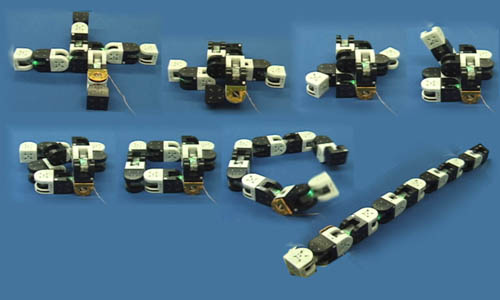
\includegraphics[width=0.6\textwidth]{images/Intro_mtran3.jpg}
        \caption{M-TRAN III modular robot reconfiguring from quadruped to snake robot.}
        \label{fig:intro_mtran3}
\end{figure} 


 In general, modular robots are used in applications in which the operating conditions of the robot are not known when the robot is to be designed, such as space exploration, battlefield reconnaissance, finding victims among the debris in natural catastrophes and other similar tasks involving complicated terrains.\\

As the robot does not rely on a single module, modular robots are fault-tolerant, and most of the robot functionality will remain even when some modules fail. Those bad-functioning modules can be substituted by other new modules, giving self-reconfigurable modular robots the property of self-repairing.\\

Modular robots can generally be classified by the arrangement of their basic unit in lattice type, chain type or hybrid type. Lattice modular robots have modules arranged in some regular pattern along 3D space, resembling atoms in crystals and they can move by changing the position of the individual modules in that lattice. In chain (or tree) modular robots the modules are connected forming strings or trees, allowing this kind of robots to reach any point of the space. Hybrid modular robots can behave as lattice type or chain type, combining the fast reconfiguration of the lattice modular robots with the ability of reaching any point of the chain type robots.\\

Modular robots can be also classified by their shape and functionality in homogeneous modular robots, in which all the unit modules follow the same design and heterogeneous modular robots, whose modules are different and each one is specialized in certain functions.\\

\begin{figure}[h]
		\centering
        \begin{subfigure}[b]{0.45\textwidth}
                \centering
                \includegraphics[width=\textwidth]{images/Intro_snake_CMU.jpg}
                \caption{Locomotion through unstructured terrains.}
                \label{fig:intro_snake_cmu}
        \end{subfigure}
        ~
        \begin{subfigure}[b]{0.45\textwidth}
                \centering
                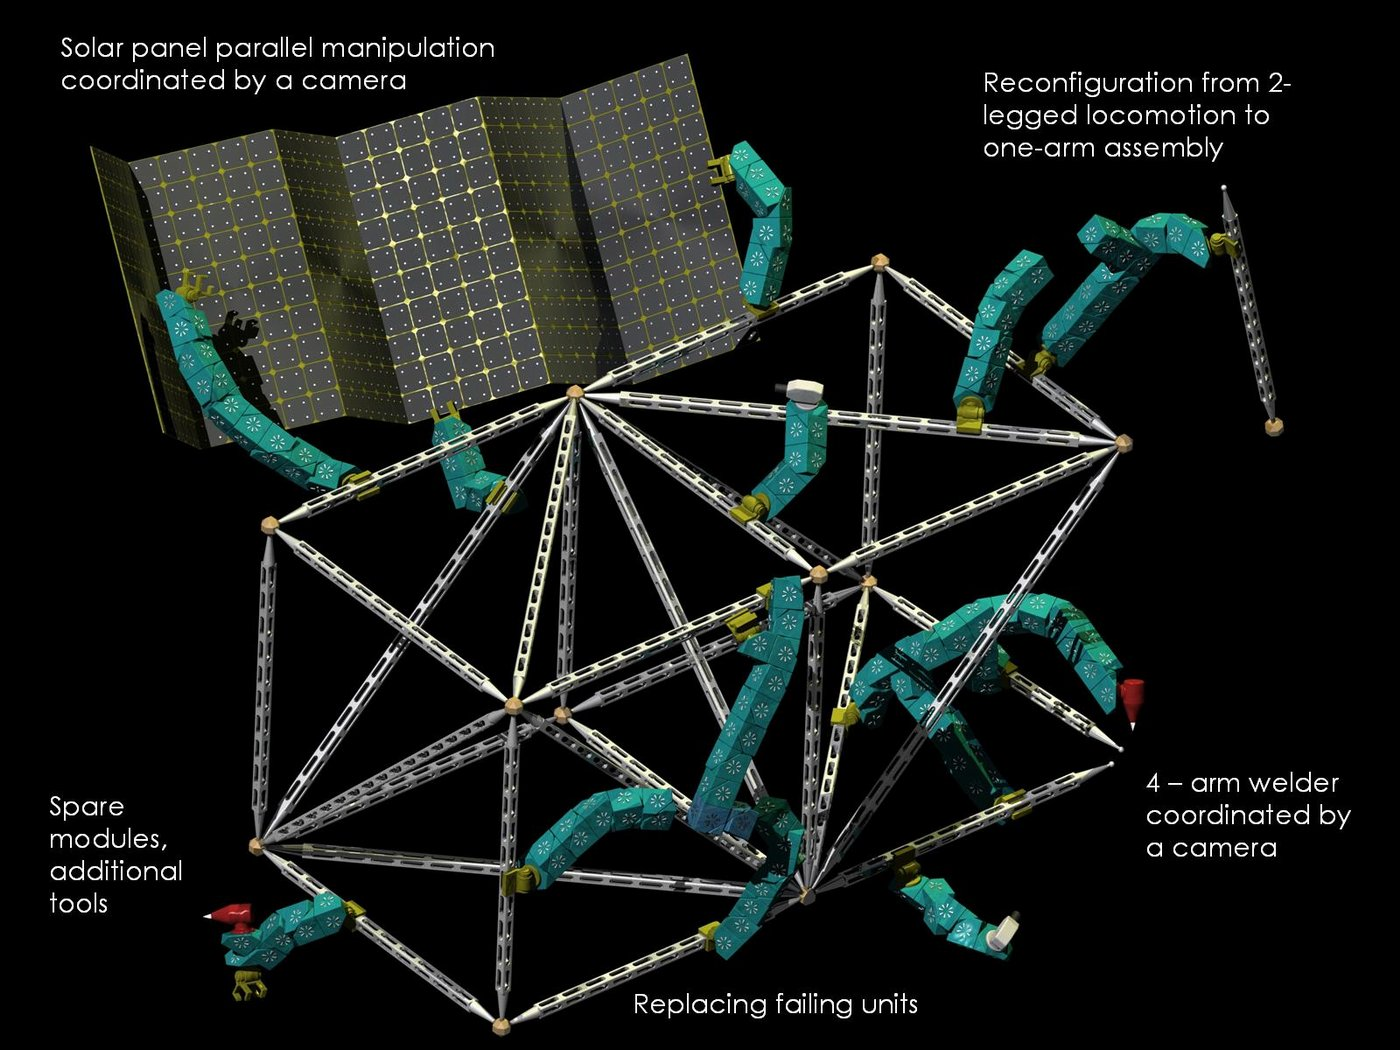
\includegraphics[width=\textwidth]{images/Intro_molecubes.jpg}
                \caption{Space applications.}
                \label{fig:intro_space_applications}
        \end{subfigure}
        \caption{Typical applications of modular robots.}
        \label{fig:intro_applications}
\end{figure}

In homogeneous modular robots, mass production can lower the cost of the robots, as they are all identical. But as currently these robots are used mainly for research, they are not mass produced, and usually very small batches of prototypes are manufactured. As each module is an autonomous robot, and therefore they need to have their own controller hardware and software, actuators (like motors), sensors, communication hardware and batteries, modular robots are usually very expensive, the cost of one single module has to be multiplied several times, increasing rapidly the cost of the robot.\\

Despite their versatility in uncertain situations, due to the high number of modules that compose a modular robot, they are usually hyper-redundant robots, robots with a large or infinite number of degrees of freedom. This complicates the search for adecuate locomotion gaits due to the increase in complexity to find the inverse kinematics of the robots, as well as the increase in difficulty of coordinating the movement of all the joints. \\

Other problem that arises in modular robotics is the distributed nature of the system, that requires each module to have its own controller, which has to interact with the other modules controllers in order to achieve a correct and optimal behavior of the whole modular robot. In this aspect, having a homogeneous controller (i.e. all the modules share exactly the same controller) eases the development and mainteinance of the controller, but a proper, scalable controller and communication protocol is still required for collaboratively control the entire robot.\\

In this thesis we address those three problems described: locomotion gait generation on a modular robot, designing a homogeneous distributed controller that can control the whole modular robot selecting the most appropiate gait for each configuration, and the development of a cheap and simple modular robot platform to test and validate locomotion gaits and controllers.\\ 

\section{Objectives}
\label{introduction_objectives}

The main objective of this thesis is to solve some of the problems in modular robotics mentioned in the introductory section. More precisely, to develop a homogeous distributed controller and optimal locomotion gaits that allow a modular robot to move as fast as possible adapting its gaits to its current configuration, and test this controller on both a simulated and a real modular robotic platform.\\

In order to achieve that objective successfully, we have divided it into four main objectives:
\begin{enumerate}
	\item \textbf{To find optimal locomotion gaits} for at least three different modular robot configurations by means of stochastic optimization algorithms.\\
	
	\item \textbf{To develop a homogeneous, distributed controller and communication algorithm} that allows a modular robot to discover its current configuration and select the most suitable gait for that configuration. \\	

	\item \textbf{To develop a software framework} that allows to simulate the modular robot and test the obtained optimal gaits, as well as the homogenous controller for their validation. This framework should be flexible enough to serve as a base for the development and testing of other controllers and configurations in the future.\\
	
	\item \textbf{To develop a cheap hardware platform} for testing the obtained optimal gaits and the distributed controller on the real world. This includes the design of both the mechanical part of the module as well as the control electronics, and the later assembly of the different configurations of the modular robot. This platform should also be upgradeable and reusable in future research related to modular robots.\\
\end{enumerate}

\newpage
\section{Phases of the project}
\label{introduction_phases}

\noindent
A brief description of the different phases of this project is presented here chronologically ordered:

\begin{enumerate}
	\item \textbf{Study of the existing work on the topic.}
		\begin{enumerate}
			\item Study of the state of the art on modular robotics.
			\item Test existing open source modular robotics platforms.
			~\\
		\end{enumerate}
		
	\item \textbf{Development of basic software framework for simulation.}
		\begin{enumerate}
			\item Development of basic digital model of the module to be used.
			\item Select and setup simulator.
			\item Development of the basic software for the control of the modular robot on the simulation.
			~\\
		\end{enumerate}				
		
	\item \textbf{Optimization of modular robot gaits.}
		\begin{enumerate}
			\item Study and selection of stochastic optimization algorithm to be used.
			\item Optimization of gaits for the main configurations to be studied.
			~\\
		\end{enumerate}
	
	\item \textbf{Development of the distributed control algorithm.}
		\begin{enumerate}
			\item Develop the theoretical distributed control algorithm for configuration discovery and gait selection.
			~\\
		\end{enumerate}
		
	\item \textbf{Development of the remaining software framework for testing the gaits and distributed controller.}
		\begin{enumerate}
			\item Development of the software related to the communication between modules.
			\item Development of the distributed controller for the module.
			\item Testing of the controller and gaits on the simulated modular robot.
			~\\
		\end{enumerate}

	\item \textbf{Development of the hardware platform for testing the gaits and distributed controller.}
		\begin{enumerate}
			\item Design, manufacturing and assembly of the control board.
			\item Design, manufacturing and assembly of the mechanical module.
			\item Assembly of the different modular robot configurations.
			\item Test of the locomotion gaits and distributed controller on the physical modular robot.
			~\\
		\end{enumerate}
		
	\item \textbf{Results documentation}
		\begin{enumerate}
			\item Comment and document software.
			\item Upload software and hardware designs to online repositories under a open source license.
			\item Write and defend thesis.
		\end{enumerate}
		
\end{enumerate}
\chapter{State of the Art}
\label{state_of_the_art}

In this chapter we will present the state of the art on the field of modular robotics. More precisely, we will discuss the state of the art of the main modules used in modular robotics research, from which we took inspiration to design our platform; the state of the art of the controllers used for achieving locomotion on chain-type modular robots and the state of the art of modular robotics communications.\\


\section{Modular Robotic Platforms}
\label{state_art_modules}
This section summarizes the current development in modular robotics, showing the most significant modules in the field, as well as the most related to the design developed by the author, and presented in chapter \ref{hardware_chapter}.

%%%% PolyPod %%%%%%%%%%%%%%%%%%%%%%%%%%%%%%%%%%%%%%%%%%%%%%%%%%%%%%%%%%%%%%
\subsection{PolyPod}
\label{state_modules_PolyPod}

PolyPod \cite{Yim1994, Yim1993} is a modular robot created by Mark Yim in 1994 for his PhD thesis, and can be considered the first robot created with the modular robotic paradigm in mind.\\

PolyPod is a heterogeneous system made of two different types of modules, called ``segments'' and ``nodes''. ``Segments'' are two degree of freedom parallel mechanisms composed of 10 links, resulting in a mechanism similar to two prismatic joints joined together by a revolute joint where the prismatic joints are constrained to have the same length. One of the degrees of freedom is linear, contracting and expanding the module from 1 inch up to 2.5 inches, and the other a revolute joint with a range of $[-45, 45]$ degrees. They also have 2 connectors that allow linear configurations and, in order to enable non-serial configurations, ``Nodes'' are used. ``Nodes'' are squared modules of aproximately 5cm x 5cm x 5cm with 6 connection ports that contain the gel-cell batteries for powering the robot.\\

PolyPod has dynamic reconfigurability, it can change its own shape by itself, adopting the configuration most suitable for each task.\\

\begin{figure}[h]
        \centering
        \begin{subfigure}[b]{0.3\textwidth}
                \centering
                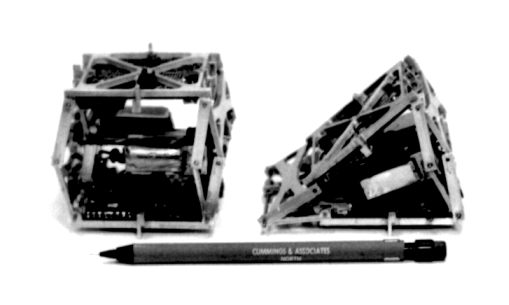
\includegraphics[width=\textwidth]{images/State_art_PolyPod.png}
                \caption{PolyPod segments}
                \label{fig:state_art_polypod-01}
        \end{subfigure}%
        ~ 
        \begin{subfigure}[b]{0.3\textwidth}
                \centering
               	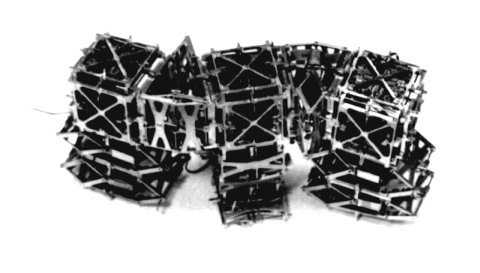
\includegraphics[width=\textwidth]{images/State_art_PolyPod-2.png}
                \caption{Robot made of PolyPod modules}
                \label{fig:state_art_polypod-02}
        \end{subfigure}
        \caption{PolyPod}
        \label{fig:state_art_polypod}
\end{figure}
%%%% polyBot %%%%%%%%%%%%%%%%%%%%%%%%%%%%%%%%%%%%%%%%%%%%%%%%%%%%%%%%%%%%
\subsection{PolyBot}
\label{state_modules_PolyBot}

\begin{figure}
        \centering
        \begin{subfigure}[b]{0.3\textwidth}
                \centering
                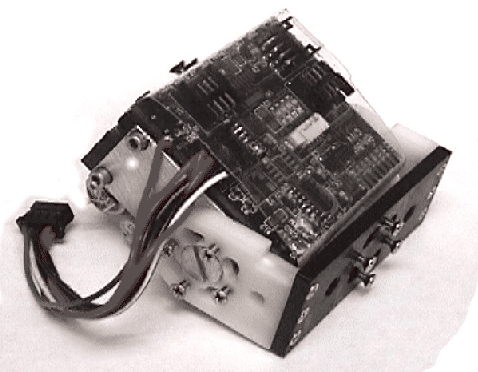
\includegraphics[width=\textwidth]{images/PolyBot_G1v4.png}
                \caption{G1v4}
                \label{fig:G1v4}
        \end{subfigure}%
        ~ 
        \begin{subfigure}[b]{0.3\textwidth}
                \centering
               	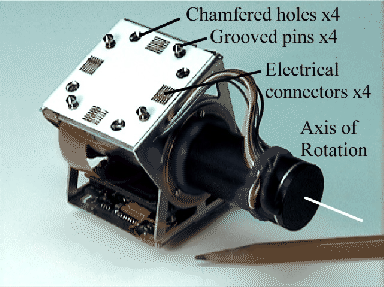
\includegraphics[width=\textwidth]{images/PolyBot_G2.png}
                \caption{G2}
                \label{fig:G2}
        \end{subfigure}
        ~
        \begin{subfigure}[b]{0.3\textwidth}
                \centering
                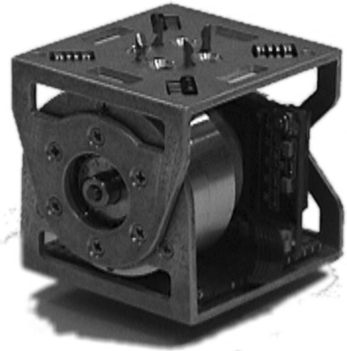
\includegraphics[width=0.8\textwidth]{images/PolyBot_G3.png}
                \caption{G3}
                \label{fig:G3}
        \end{subfigure}
		\caption{Three generations of PolyBot modules}\label{fig:PolyBot}
\end{figure}

PolyBot\cite{yim_modular_2003} is a modular robot developed by Mark Yim at the Palo Alto Research Center (PARC), as the evolution of the PolyPod robot. It has been designed with space missions in mind, resulting in a small and light module. It is currently formed by G3 modules, which are the third generation of modules developed for PolyBot. 
\\

The first generation modules were simple modules with one degree of freedom made from laser cut plastic with genderless symmetric passive connectors joined by screws, and a hobby servo for joint motion. They were not able of self-reconfiguration and the power and computations were given externally.
\\

The second generation modules were made from laser cut stainless steel, and the joint was actuated through a brushless motor that laid partially outside the module body due to the size of the gearbox. The connector was also upgraded with IR sensors and shape-memory alloy actuators for self-reconfiguration and active attachment/detachment. Communication among modules was carried through two CAN buses.
\\

For the third generation of modules, a smaller custom made gearbox was added to the brushless motor so that it would be contained inside the module. Power consumption was reduced and several improvements were introduced to the connectors, allowing them to make passive connections and increasing the IR accuracy.
\\


%%%% Conro %%%%%%%%%%%%%%%%%%%%%%%%%%%%%%%%%%%%%%%%%%%%%%%%%%%%%%%%%%%%%%
\subsection{CONRO}
\label{state_modules_CONRO}

\begin{figure}[b]
	\centering
	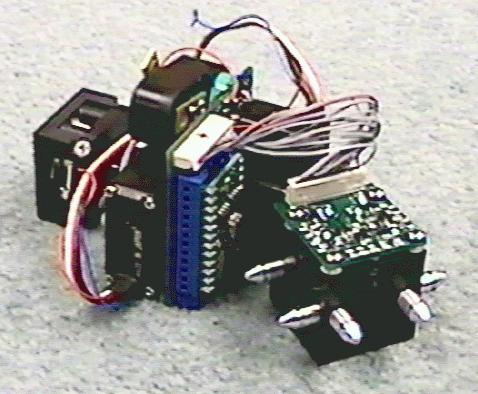
\includegraphics[width=0.3\textwidth]{images/CONRO01.jpg}
	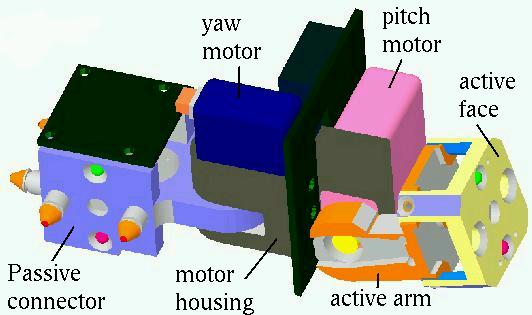
\includegraphics[width=0.3\textwidth]{images/CONRO02.jpg}
	\caption{CONRO module}\label{fig:conro}
\end{figure}
CONRO\cite{castano_conro_2002} is a self-reconfigurable robot developed at the University of Southern California with search, rescue and surveillance operations in mind. The modules for the CONRO robot are fully autonomous, and are divided into three main sections: a passive connector, an active connector and the main body. 
\\

The passive connector is a plastic cube with a pair of pins in three of its faces. These pins are made from aluminium and have a cylindrical shape, with a groove to allow the active connector to lock them. The passive connector is hollow, and holds two 160mAh lithium batteries of 3V and 6V and the IR serial communication trasmitters, receivers and control circuitry, which allows the module to communicate with its neighbours when connected and also in the docking process. The IR system also works as a position feedback information to position the modules correctly while docking.
\\

The main body holds two hobby servo which are connected with the passive and active connectors respectively and provide two degrees of freedom for the module. The body also contains the control board, which as a zero insertion force socket that allows the module to use three different microprocessors depending on the task requirements: a Stamp II based on a PIC16C57 or a Stamp IIe or II-SX based on a SCENIX SX28AC/SS processor.
\\

Finally, the active connector is equipped with a pair of holes for the passive connector pins and a latch for holding the modules together. Connection of the two modules is passive, whereas a shape-memory allow wire allows the disconnection of the module.


%%%% Superbot %%%%%%%%%%%%%%%%%%%%%%%%%%%%%%%%%%%%%%%%%%%%%%%%%%%%%%%%%%%
\subsection{Superbot}
\label{state_modules_Superbot}

\begin{figure}[h]
	\centering
	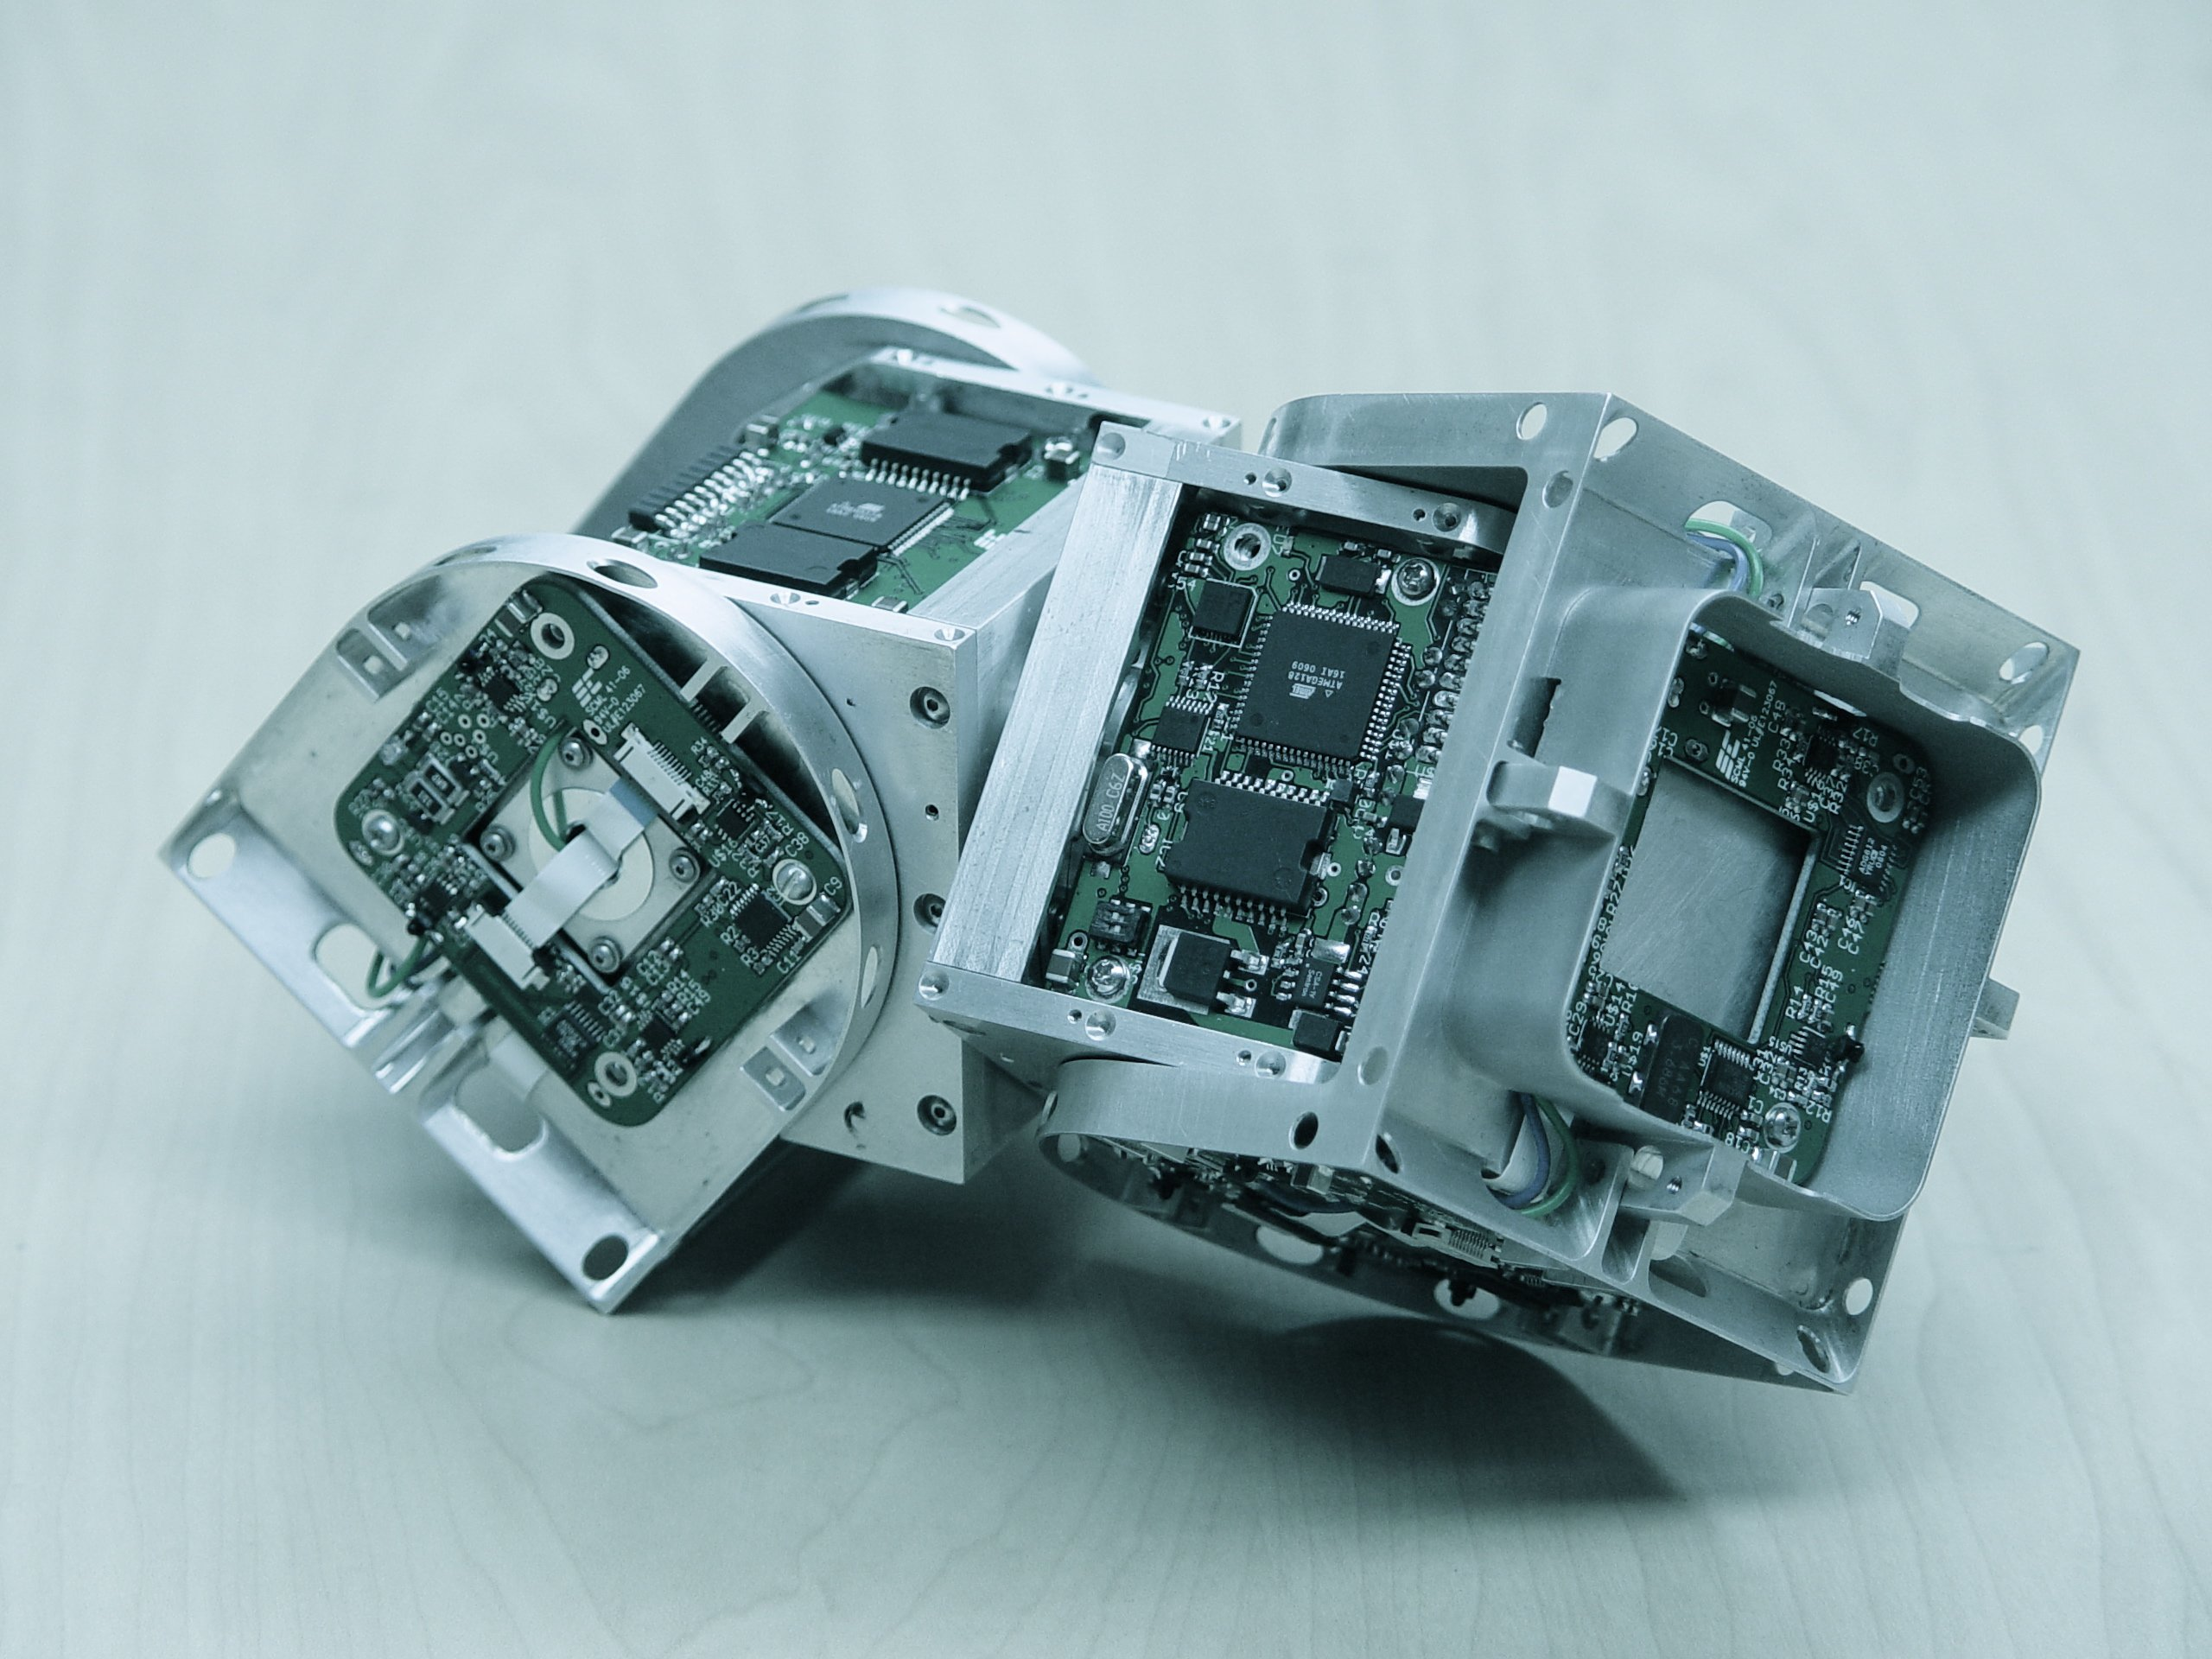
\includegraphics[width=0.3\textwidth]{images/Superbot01.JPG}
	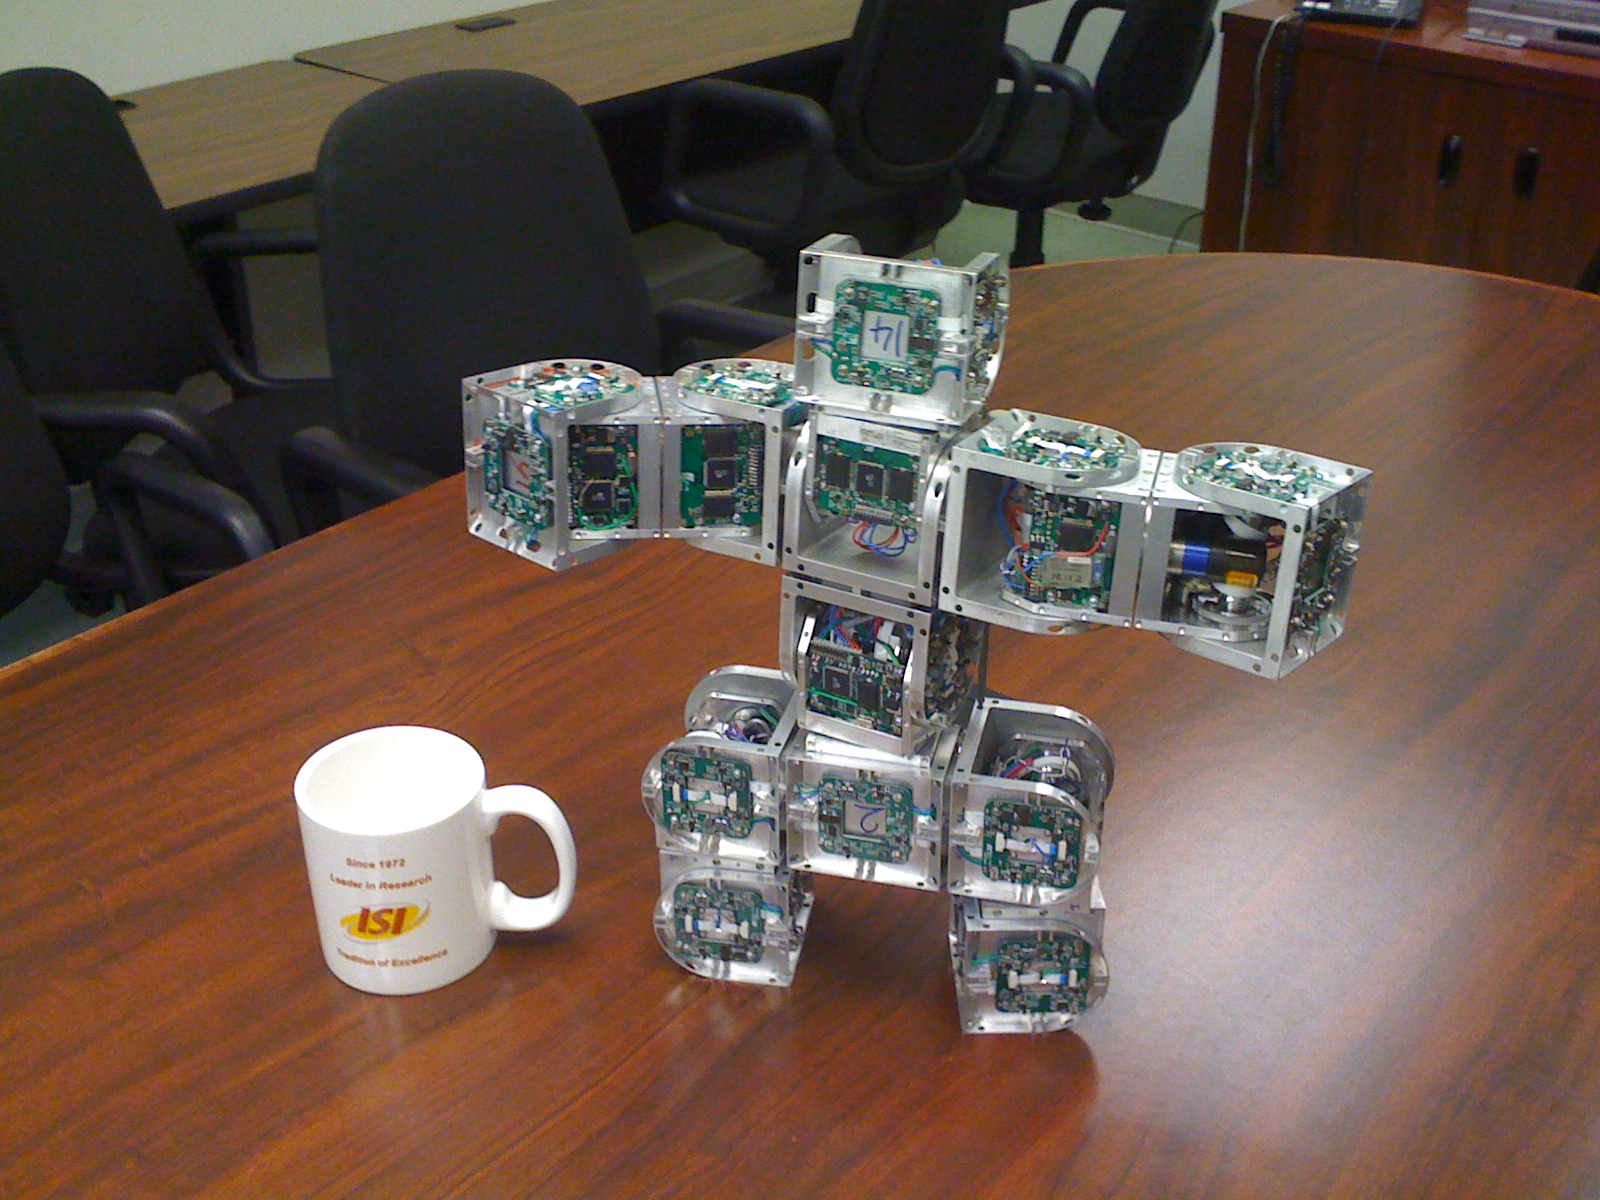
\includegraphics[width=0.3\textwidth]{images/Superbot02.JPG}
	\caption{Superbot module}\label{fig:superbot}
\end{figure}


The Superbot\cite{salemi_superbot:_2006} modular robot is the descendant of the CONRO module, and has been developed by the Polymorphic Robotics Laboratory at the University of Southern California. Funded by the NASA to be used for space applications, it is a hybrid module, as it can perform as a chain-type module or a lattice-type module.
\\

Superbot modules are made from two cube-like bodies of 84x84x84mm that have each one a degree of freedom. The joint between both cubes can rotate about 270º so it has a total of three degrees of freedom, which allows the module to move freely on a plane.
\\

Each degree of freedom is actuated by a DC motor equipped with a planetary gearbox and an external gearbox, and controlled by a software PID which recieves the feedback information from a potentiometer coupled to the motor shaft.
\\

The electronics design is modular and the main circuitry is divided into two boards, a master board on one half of the module, and a slave board on the other half. Each board has an ATmega128 microcontroller and both are connected through a I2C bus. Each one of the six connectors of the module has an IR communication system that allows communication with it neighbors and provide position and distance feedback for docking with other modules. 
\\

Power is supplied to the module by a 1600mAh, 7.4V lithium-polymer battery, and can be shared to the neighboring modules when needed through the connectors. This sharing process is controlled as a high-level routine by the microcontroller that manages this functionality.
\\

%%%% M-TRAN %%%%%%%%%%%%%%%%%%%%%%%%%%%%%%%%%%%%%%%%%%%%%%%%%%%%%%%%%%%%%
\subsection{M-TRAN}
\label{state_modules_M-TRAN}

\begin{figure}[t]
	\centering
	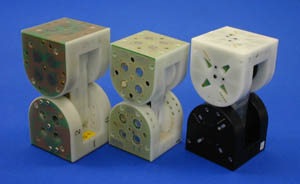
\includegraphics[width=0.3\textwidth]{images/M-TRAN01.jpg}
	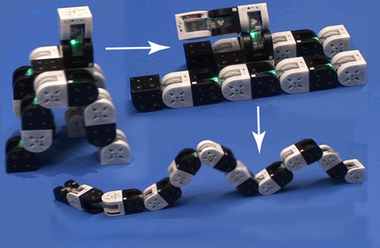
\includegraphics[width=0.3\textwidth]{images/M-TRAN02.jpg}
	\caption{M-TRAN module}\label{fig:m-tran}
\end{figure}

M-TRAN (Modular TRANsformer) \cite{murata_m-tran:_2002,kurokawa_m-tran_2003,kurokawa_distributed_2008} is a self-reconfigurable robot being developed by AIST and Tokyo-Tech since 1998. Their third and latest iteration of the robot is called M-TRAN III. M-TRAN is a hybrid module able to perform as a lattice-type modular robot for reconfiguration and as a chain/tree type for displacement.
\\

The module is made from two semi-cylindrical boxes and a link joining them together. One of these boxes is active, and has three connectors with hooks that are able to connect with the passive box of the other modulues. This design improves the previous one (used in M-TRAN and M-TRAN II) that used permanent magnets for connection and a shape-memory alloy coil for detachment, as it is several times faster (around 5 seconds for M-TRAN III system versus nearly 1 minute for the previous systems). Each box is able to rotate 180º around its joint with the link, giving M-TRAN a total of 2 parallel degrees of freedom. While in lattice mode, this joints are actuated only in multiples of 90º, allowing a checkerboard pattern in which active connectors coincide with passive connectors for reconfiguration.
\\

For the robot control, M-TRAN has four microcontrollers in total: one as master, that carries the main high-level behaviour and three slaves, that are in charge of several subsystems as the motor control, the communication system or sensors like the 3-axis accelerometer. It has several communication methods, such as bluetooth, IR and even a physical CAN bus through some pins on the connectors, which allows the modules to communicate no matter if they are physically in contact or in different assemblies.
\\

A battery and a power supply circuit are placed in the passive box of the M-TRAN module, supporting autonomous operation.



%%%% Y1 %%%%%%%%%%%%%%%%%%%%%%%%%%%%%%%%%%%%%%%%%%%%%%%%%%%%%%%%%%%%%%%%%
\subsection{Y1}
\label{state_modules_y1}


\begin{figure}[b]
		\centering
        \begin{subfigure}[b]{0.3\textwidth}
                \centering
                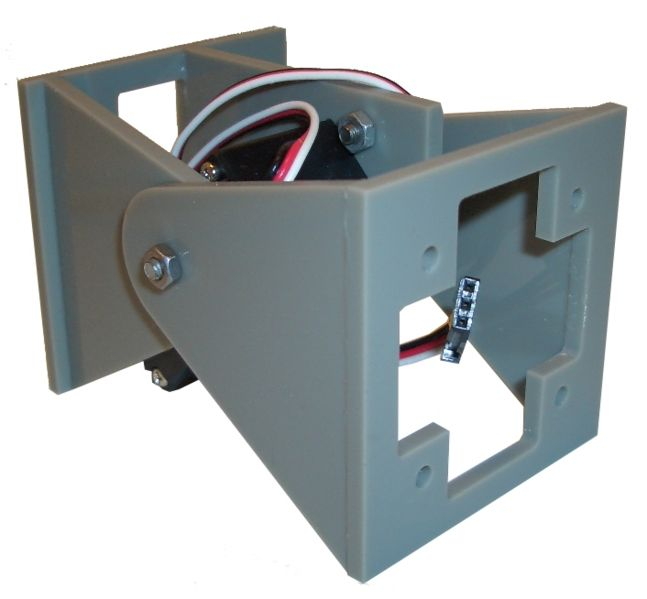
\includegraphics[width=\textwidth]{images/Y1_01.jpg}
                \caption{Y1}
                \label{fig:state_art_y1_mod}
        \end{subfigure}
        ~
        \begin{subfigure}[b]{0.3\textwidth}
                \centering
                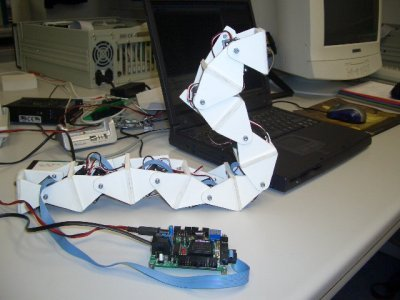
\includegraphics[width=\textwidth]{images/State_art_Y1_cube.jpeg}
                \caption{Cube Revolutions (Y1 snake)}
                \label{fig:state_art_y1_cube}
        \end{subfigure}
        \caption{Y1} \label{fig:state_art_y1}
\end{figure}

Y1\cite{gonzalez-gomez_website:y1} modules were developed by Juan Gonzalez-Gomez at the Autonomous University of Madrid based on the first generation of PolyBot modules. The main objective of the Y1 modules was to create a cheap and open platform for researching modular robotics.
\\

The Y1 modules are composed of a cheap hobby servo and a two-part housing made from laset cut PVC. This modules can be connected in a linear configuration, either pitch-pitch or pitch-yaw, allowing the resulting robots to move in a plane. Reconfiguration has to be done by hand, as the modules are joined by means of screws. The control electronics and the power source are supplied off-board.
\\

The Y1 module is open source hardware, which means that the plans, the files for manufacturing and the assembly instructions are available online for anyone to access to them. 
\\

The REPY-2.1 module developed by us and used for testing the gaits of this thesis is based on the Y1 module. More details about the Y1 and REPY-2.1 modules can be found in chapter \ref{hardware_chapter}.



%%%%%%%%%%%%%%%%%%%%%%%%%%%%%%%%%%%%%%%%%%%%%%%%%%%%%%%%%%%
%%%%%%%%%%%%%%%%%%%%%%%  GAITS  %%%%%%%%%%%%%%%%%%%%%%%%%%%
%%%%%%%%%%%%%%%%%%%%%%%%%%%%%%%%%%%%%%%%%%%%%%%%%%%%%%%%%%%
\section{Gait Generation on Modular Robots}
\label{state_art_controllers}

The lower level control for locomotion in mobile robots with wheels or tracks is usually not complicated, since it only involves turning the motors in order to produce movement. Difficulties appear at the higher level control, such as motion planning or navigation.\\

But, when the robot is articulated, either with legs or apodal, the lower level control becomes more complicated, as the problem of coordination appears, even if the robot is to travel through a flat surface without any kind of obstacles. In this kind of robots the movement of each of the joints must be coordinated with the movement of the other joints so that the robot can move. In more formal terms, the coordination problem can be stated as follows: \emph{For a robot with N articulations, find the value of each joint as a function of time $\varphi_i(t)$ so that the robot can achieve locomotion}. The solution of this problem is not unique, and depends on the type of gait that one desires to obtain (e.g. walking on a straight line, turning, trotting, galloping, etc).\\

In order to solve this problem, several approaches can be found in the literature, and they will be explained in this section.\\

\subsection{Gait tables}
\label{gait_gaittables}

Gait tables are tables that include the joint position values for each module at different steps of a gait. For each moment of the gait, each of the modules look up in the table what is the required joint value for the current step, and move their joints to that value. When the robot arrives at the end of the table, it starts again with the first position of the table, achieving a repeating pattern.\\

This is an easy and simple way to implement locomotion gaits for modular robots, and was first used by Mark Yim in his PolyPod \cite{Yim1993}. When the robots are composed of few modules and the desired movements are simple, these gait tables can be formed by hand, allowing a fast exploration of possible gaits for locomotion, as well as detecting mechanical defects on robot prototypes. Gait tables are not only useful for designing gaits for modular robots, but they can also be applied to other types of robots, such as quadruped, hexapods or even humanoid robots.\\

The main disadvantage of gait tables is that they lack flexibility, as for generating new gaits, or variations of the existing gaits, a new control table has to be created.\\

\subsection{Central Pattern Generators (CPGs)}
\label{gait_cpgs}
Central pattern generators (CPGs) are biological neural networks capable of producing coordinated patterns of rhythmic activity without any rhythmic inputs from sensory feedback or from higher control centers \cite{Ijspeert2008}. They are in charge of many rhythmic behaviours in both vertebrate and invertebrate animals, such as breathing, locomotion, bowel movements, etc.\\

CPGs are distributed networks composed by multiple coupled oscillatory centers, as observed in experiments with lampreys and salamanders, in which small sections of their spinal cords were capable of producing rhythmics activity. The lamprey is one the vertebrates most used to study CPGs, because its spinal column is transparent, contains few cells, and lasts at least a week outside
of the animal (in a saline solution) without deterioration \cite{Rovainen1979}, easing the work of the biologists.\\

Sensory feedback is not needed for the generation of the rhythms, but plays a key role in shaping the rhythmic patterns and keeping the body movements and the CPG coordinated. This coupling is so tight that is posible to induce CPG activity mecanically moving the tail of a lamprey, and to induce a normally looking walking gait in a decerebrated \footnote{Decerebration is the elimination of cerebral brain function in an animal by removing the cerebrum, cutting across the brain stem, or severing certain arteries in the brain stem \cite{decerebration}.} cat by placing it on a treadmill. If the treadmill is accelerated, the gait can even change from trot to gallop.\\

The complex locomotion behaviour generated by the CPG circuits is controlled by simple signals, that in many vertebrates are generated in a specific region of the brain stem known as \emph{Mesencephalic Locomotion Region} (MLR). Some experiments with electrical stimulation of this region have shown that the level of stimulation can modulate the speed of locomotions, and induce an automatic gait transition (from walk to trot to gallop on derebrated cats, and from walk to swimming on decerebrated salamanders). Therefore, basic rhythmic patters are generated at the spinal CPGs, but the modulation of those patterns according to environmental factors is controlled by the higher-level centers, such as the motor cortex, cerebellum and basal ganglia.\\

These biological CPGs have been matematically modelled as differential equations, and successfully applied to different robots, such as the \emph{Salamandra Robotica}, a salamander-like robot developed at the EPFL \cite{Ijspeert2007}. Since CPGs are a distributed approach, it has been also applied to modular robots, such as YaMoR \cite{Marbach2005} or the Roombots \cite{Sprowitz2010}. One advantage of using CPGs is that the transition between two steady state oscillations is bounded, continuous and relatively smooth, so if we are implementing an optimization algorithm for the gaits, and we randomly change the control parameters, the joint values will not change too abruptly, which helps preventing the motors from breaking \cite{Ijspeert2008}.\\

\subsection{Sinusoidal Oscillators}
\label{gait_sin_osc}

CPGs are very powerful, but they are complex and require lots of computing power. For that reason some researchers tried to substitute on their controllers the CPG model obtained by neurocomputing scientists by a simpler one that performs in a similar way, but using less resources. CPGs behave as fixed frequency oscillators in steady state, making sinusoidal oscillator a suitable canditate for being used as gait generators, as they are much simpler to model and require less resources for their implementation than CPGs. Implementations of sinusoidal oscillators have been tested successfully on snake robots by Lipkin et al., who also defined piecewise functions to perform specialized tasks, such as stair climbing \cite{Lipkin2007}, and Gonzalez-Gomez \cite{Gonzalez-Gomez2008}, who also studied the minimal configurations required for locomotion with sinusoidal oscillators \cite{Gonzalez-Gomez2006}. Sinusoidal oscillators also been applied to legged robots such as the hexapod robot Melanie-III with success \cite{AlonsoPuig2005}.\\

Other approaches simplify even more the coupled oscillators of the CPG approach, substituting them by a single sinusoidal waveform as a function of time and current module, that is used to control the all the joint positions \cite{Tesch2009}.\\

Due to its simplicity, sinusoidal oscillators are the approach selected in this thesis to solve the coordination problem, and are described in detail in chapter \ref{config_gait}.\\

\section{Coordination and Communications on Modular Robots}
\label{state_art_coordination}

Communication between robots is essential for achieving coordination. This becomes of special importance when working with modular robots, as because of their nature, they require their modules to colaborate with each others to complete a task. In order to achive reconfiguration or locomotion the modules need to know what their positions inside the modular robot are, what tasks or steps have been completed and which remain still pending for completion. \\

On modular robots, these communications are implemented on hardware in very different ways. Some of them, such as PolyPod, M-TRAN or SYMBRION / REPLICATOR have physical connectors that are used for communication when two modules are attached together \cite{Yim2000, Kurokawa2008, Liedke2011}, whereas most of the existing modules, such as CONRO, SUPERBOT or ATRON, communicate using IR or IrDA communications \cite{Castano2000, Salemi2006, Brandt2007}, which have the advantage of being wireless and that can be also used as distance sensors. A few modules, such as YaMoR or M-TRAN, can communicate using Bluetooth communications, allowing modules that are not physically attached to interact with each other\cite{ Mockel2006, Kurokawa2008}.\\

Communications between robots can be classified as global or local communications. In local communications, robots only talk to their nearest neighbors and information is shared locally. This approach is tipically used in modular robotics to find the topology of the robot and to coordinate local tasks. On the other hand, when using global communications all modules can communicate between each other and achieve coordination of tasks involving distant modules.\\

The type of communications a certain module can perform conditions its control strategy, modules with a global communication system usually apply centralized control methods, such as PolyPod's central gait tables\cite{Yim2000} or M-TRAN's centralized central pattern generators\cite{Kamimura2005} whereas modules with local communications tipically use distributed control methods, like CONRO's and SUPERBOT's distributed digital hormones \cite{Shen2002}.\\

Local communication methods are used mainly for coordination of reconfiguration in lattice-type modular robots and for coordination and synchronization of locomotion movements in chain-type modular robots. Butler et al. described a renconfiguration method for lattice modular robots using only local information based on cellular automata, a simple set of rules that control the reconfiguration steps depending on the neighbors attached to the module, and on the obstacles detected, allowing a flow-like locomotion\cite{Butler2004}. Funiak et al. presented a distributed method for module location inside large modular robots, consisting in breaking the cluster of modules in smaller clusters using normalized cut to identify dense sub-regions with small mutual localization errors\cite{Funiak2009}.\\

For locomotion synchronization and coordination the most notable distributed approach is digital hormones. Digital hormones are a nature-inspired communication method published by Shen et al., based on biological hormones, that consist on signals or messages that are propagated by the modular robot, triggering different actions depending on the function of the module that receives them. Those local actions are executed by the modules without the help of the hormone, and include joint movement and hormone manipulation and destruction, among others \cite{Shen2000}.\\

For this thesis digital hormones were selected as communication method due to their proved usefulness in distributed control of locomotion in chain-type robots \cite{Shen2002, Hou2006}. Digital hormones and our developed algorithm will be described in detail on chapter \ref{hormones}.\\

\chapter{Software}
\label{software_chapter}

In this chapter we will describe and explain the software framework implemented to work with modular robots and test the locomotion gaits and digital hormone-based controller. This framework is named	\emph{Hormodular}, a combination of the terms ``hormone'' and ``modular''.\\

All the software developed for the \emph{Hormodular} framework is open source, and can be found in the following github repository: \url{https://github.com/David-Estevez/hormodular}. Being open source, anyone can download, use and study the code freely. This is very important in research, as any researcher interested in modular robotics in any part of the world can use this code, learn from it, improve it or repeat the experiments described in this thesis to test the validity of the results presented here.\\

This chapter will start explaining what are the software dependencies used in this project, then we will describe the Test-Driven Development methodology followed to develop the project. Next, the software structure will be discussed, with a detailed description of all the different classes implemented. Finally, the compilation procedure and program usage are offered for anyone interested on downloading and using this software.\\


\section{Software dependencies}
\label{software_dependencies}

Due to the complexity of the project, some specific tasks required the use of third-party libraries perform them. According to the open source nature of our project, these libraries were chose to be also open source, and compatible with GNU/Linux systems. These libraries are in charge of tasks such as simulation of the modular robot, optimization of the oscillator parameters in order to achieve locomotion or parsing XML configuration files.

\subsection{Simulation software: OpenRAVE}
\label{software_openRAVE}

The simulation software used by the student for this project is OpenRAVE. OpenRAVE \cite{diankov_thesis} is an Open Source project developed by Rosen Diankov that provides simulation tools for working with robots and trajectory planners. It can be embedded on other controllers and larger frameworks, and its functionality can be extended by means of plugins, adding new trajectory planners, controllers, collision checkers, inverse kinematics solvers, robots or sensors as needed.\\

OpenRAVE was chosen over other simulators due to its open source nature and its extensive documentation \cite{diankov_website:openrave}, as well as its easy integration with larger projects, such as this one.

\subsection{Modular Robotics plugin for OpenRAVE: OpenMR}
\label{software_openMR}

OpenMR \cite{gonzalez-gomez_website:openmr} is a plugin for the OpenRAVE simulator developed by Juan Gonzalez-Gomez that allows the user to simulate servo motors on the joint of OpenRAVE robots.\\

It adjusts the angular velocity of the robot joint by means of a PD controller feedbacked with the joint angular position, so that the user can control the joint position value with a simple interface.

\subsection{Evolutionary Computation Framework: ECF}
\label{software_ECF}

The Evolutionary Computation Framework (ECF) \cite{ecf:website} is a C++ library that allows the user to apply several evolutionary optimization algorithms in a very customizable way. It offers several common evolutionary optimization algorithms such as particle swarm optimization (PSO), differential evolution (DE), genetic annealing, artificial bee colony (ABC), and genetic algorithms with steady state tournament and generational roulette-wheel selection, among others.\\

By means of a XML file, the user selects the optimization algorithms to be used, and its parameters. That XML file also contains information about the genotype that will encode the different parameters to be evolved. The user can specify his own fields that can be later read by the software containing the ECF to set user-defined paramters.\\

The interface of the ECF is very simple, and to optimize a given function the user just has to inherit from the base class ``EvaluateOp'', registering the custom parameters needed by that class to be extracted from the configuration XML file, and specifying the actions to me made for the initialization and evaluation of the function with a given genotype.\\

In this case the function to be evaluated is the distance travelled by the modular robot running for a certain period of time using the oscillator parameters specified by the genotype.


\subsection{XML parsing: TinyXML2}
\label{software_tinyxml2}

TinyXML2 \cite{tinyxml2:website} is an Open Source lightweight C++ library that supports Document Object Model (DOM) parsing of XML with a very small memory footprint. DOM parsing is a cross-platform and language-independent convention for representing tagged documents such as HTML, XHTML or XML files, and means that the data inside the xml file is represented as a tree in which each node is an object that can be addressed and manipulated.\\

TinyXML2 can be easily integrated in a project with almost any configuration required. It is also has a very simple API, is fast and requires a very small amount of memory, being those the main reasons for using it in this project, instead of coding a XML parser from scratch or using a bigger XML parser.\\

XML files are used in this project for storing the robot configuration in a way that is easy for a human to setup manually, and also simple for a machine to extract that information later.\\



\subsection{Linear algebra library: Eigen}
\label{software_eigen}

Eigen \cite{eigen:website} is an Open Source C++ library for performing linear algebra operations with matrices, vectors and algorithms related to them. It is implemented as a template library that only includes header files, and supports matrices of all sizes and numeric types, including integers, floating-point numbers and complex numbers.\\

Eigen also support homogeneous transformation matrices, vector-axis pairs and quaternions, that are used in this project to obtain the relative orientation between two modules from the data obtained by the simulated IMU.\\

\subsection{Software build tool: CMake}
\label{software_cmake}

CMake \cite{cmake:website} is a cross-platform, open source build system designed to build, test and package software. Using simple and compiler-independent configuration files, CMake allows to control the build and linking process, generating all the files and environments required by the compiler chosen by the end user to build the code.\\

CMake  supports building programs that require several libraries, cross-compilation, as well as complex directory hierarchies and it is used in many large open source software projects, such as Blender, KiCAD, OpenCV, Point Cloud Library or Qt5.


\section{Development Methodology: Test-driven Development (TDD)}
\label{software_TDD}

For the development of the software of this project, the author has used a software development methodology called ``Test-driven Development (TDD)'', part of a larger set of development methods called ``Agile software development''. ``Agile software development'' methods allow a fast development of the project based on an iterative and incremental process, in which the code evolves from a simple version to the final one by adding functionality little by little as required by the project.\\

``Test-driven Development'' methodology \cite{tdd:book} is based on a short development cycle that is repeated iteratively, in which a new desired feature or improvement is used in a test case that initially fails (since there is no code for performing that feature yet). Then, the programmer implents the minimum code required to pass that test, and finally refactors the code into a clearer and more mantainable form.\\

Since every functionality in the code has a test associated, the code has a greater maintainability. Extending or improving the code becomes easier, faster and safer, since the tests can be run before commiting changes to the repository, ensuring that the new code does not break any old functionality. For example, when a team works on a software project, TDD allows them to check that the new code each member adds does not interfere with the old tested code, reducing the number of bugs and reducing the code interdependency.\\

Tests also help programmers understand the code written by other people. Since the test uses the code (functions, classes, etc) in order to test them, they can be used by programmers as a reference of how that code is supposed to be used and behave.\\

\subsection{Test-Driven Development main cycle}
\label{software_TDD_maincycle}

The main cycle of developing a new feature or improvement with a Test-Driven Development methodolody is the following:

\begin{enumerate}
	\item {\bfseries Add a test for the new feature or improvement.}\\
	When a new feature or improvement is required, a new test is written. Since there is no code yet that implement that feature, this test must fail. The test must check all the requirements of that particular feature to be added. That way, the developer can focus on the requirements and not add any unnecessary code.\\
	
	\item {\bfseries Run all tests. Check that the new one fails. }\\
	This steps checks that all previous tests pass without any issue, and that the new added test fails. The new test must fail, because there is no code yet for that feature, and that allows the developer to check whether the test was correct or not. A new test that passes without the addition of any code is useless for the programmer, since it does not check the new code to be implemented.\\
	
	\item {\bfseries Write the code for the new feature.}\\
	In this step the developer implements the minimum code required to make the test pass. This code does not need to be as eficient or elegant as the original, it just has to pass the test. This code is not definitive, and it will be improved and refined in later steps.\\
	
	\item {\bfseries Run tests.}\\
	At this point the developer has to run all the tests, including the new one. This will ensure that the code developed meets the tested requirements, and that the new code does not break any previous functionality tested in other tests.\\
	
	\item {\bfseries Refactor code.}\\
	The tested code has to be now cleaned up in order to be eficient, elegant and maintainable. In this step the code is moved to where it belongs logically within the project and encapsulated in a class if needed. If there is any duplicated piece of code, the developer should remove it, for example, by creating a function that encapsulates it. He has also to check whether the names given to functions and variables make sense and are representative of their current use. All these actions are called ``refactoring code''.\\
	
	By running againt the tests, the programmer can be confident that the refactored code still performs as required, and that the older code works as expected.\\
	
	\item {\bfseries Repeat.}\\
	Since this is an iterative process, it has to be repeated for each new feature to be added, incrementing the overall functionality of the project. These increments have to be small enough to allow a fast development and to minimize the amount of time spent in debugging the code.\\
\end{enumerate}

\subsection{Test-Driven Development example}
\label{software_TDD_example}

In order to explain better the development cycle under a ``Test-driven development'' methodology, we will present an example. In this example, we will develop a simple calculator that performs sums and wrap it on a C++ class. For the test we will use Google's GTest C++ Framework, that will be described in detail in section \ref{software_gtest}. \\

The first step is to define what is the functionality that the new code has to perform, and write the first test. In this case the functionality is to perform a simple sum, so the test will be very simple. One will usually test the error-prone or critical cases, in this case, we will test the sums of some positive numbers, the sum of positive and negative numbers, and the addition of 0. If we were developing the division function, for example, we would test the behaviour when dividing by 0, checking for example that the code raises an exception when the user tries to divide by 0.\\

The test would look like this:\\

\Cpp
\begin{lstlisting}

class TestCalculator : public testing::Test
{
	/* These class will contain the elements common to all the test, 
	but for now it is empty */
};

/* TEST_F stands for test fixture, test fixtures use a test class inheriting from testing::Test,
like TestCalculator. The first parameter is the testing::Test class to be used, and the second
one is the name of the test to be implemented. */ 
TEST_F( TestCalculator, calculatorAddsPositiveNumbers)
{
	/* EXPECT works as an ASSERT, but if the condition is not accomplished, it continues the rest
	of the test, reporting the error at the end. The expected result is placed as first argument, 
	and the expresion to be evaluated is placed as second argument.*/
	EXPECT(42, calculator.add(21, 21));
}

TEST_F( TestCalculator, calculatorAddsZero)
{
	EXPECT( 5, calculator.add(5, 0);
}

TEST_F( TestCalculator, calculatorAddsNegativeNumbers)
{
	EXPECT(-1, calculator.add(1, -2);
}
\end{lstlisting}

If we try to run this test, it will not even compile, as calculator, which is a instance of the class Calculator has not been created. In fact, the class Calculator has not been declared, so we will add it to the test, and we will instantiate it to be able to run the test:\\

\Cpp
\begin{lstlisting}
/* We add this class to the test file. Note that we did not implement the add method yet. */
class Calculator 
{
  public:
    int add( int a, int b);
};

/* We modify the test class, adding the calculator instance to be tested. */
class TestCalculator : public testing::Test
{
  public:
    Calculator calculator;
};

\end{lstlisting}

When this test is run, it should not pass any of the tests, since the functionality has not been implemented yet. Once we have checked that the test fails, we will implement the requested functionality:\\

\Cpp
\begin{lstlisting}
/* We implement the calculator class in the same file */
int Calculator::add( int a, int b)
{
    return a+b;
}
\end{lstlisting}

Running the tests now will result in all the tests passing. After this code we would refactor all the code to a more maintainable form. In case we wrote the code directly in the test, we would put it on a function or class. Since we did use a class from the beginning, refactoring will consist on moving the class to its own header file ``Calculator.hpp''. After we have refactored the code, the tests must be run again to check that the code still passes them. \\

If we want to add more features to the calculator, such as subtraction, multiplication or division, we would repeat the process again from the start, creating a new test for the new operations to be implemented.\\

\subsection{Google Test (GTest)}
\label{software_gtest}
Google Test (GTest) \cite{gtest:website} is a framework for writing tests in C++ developed used by Google in their software projects, and released publicly under a Open Source license. By means of several macros, one can add tests that are automatically discovered by GTest, as well as assertions to be ensured by the code.\\

Different tests of the same class or library can be grouped in a test fixture. As seen in the previous example (section \ref{software_TDD_example}), GTest provides a class \emph{testing::Test} that can be used to set up the data or prerequisites for the test. The programmer can define a class that inherits from \emph{testing::Test} and, before each test of the test fixture is run, the \emph{SetUp()} method implemented by the programmer will be called by GTest in order to setup the required elements used in the test. After the test is finished, the \emph{TearDown()} function will be called by GTest in order to perform the cleanup of the used elements, or to free the allocated memory.\\

Each new test is added by using the \emph{TEST()} macro, taking as argument the name of the test. If the tests are going to be grouped in a test fixture that uses the same data or instances of the class to be tested, the \emph{TEST\_F()} macro can be used instead. The \emph{TEST\_F()} macro takes two arguments: the first one is the name of the class inheriting from \emph{testing::Test} that will prepare the data for each test, and the second one is the name of the test to be implemented. GTests are recognized at compilation time, and integrated in a GTest application, that runs the tests and shows a report like the shown in figure \ref{fig:software_gtest_report}. \\

\begin{figure}[h]
		\centering
        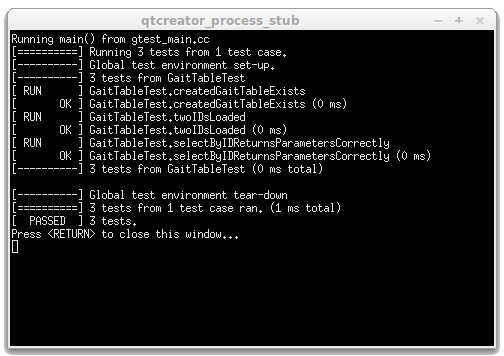
\includegraphics[width=0.6\textwidth]{images/software_gtest_report.png}
        \caption{GTest report}\label{fig:software_gtest_report}
\end{figure}

Inside the test, the conditions that have to be ensured are checked with the macros \emph{ASSERT()} and \emph{EXPECT()}. The main difference between them is that if \emph{ASSERT()} is used, the execution of the test ends if the condition imposed is not met, whereas if \emph{EXPECT()} is used instead, the execution of the test continues even thought that condition fails. One typically uses \emph{ASSERT()} when the test cannot continue if the condition fails, or if it has no sense to continue with the test if the condition fails. On the other hand, using \emph{EXPECT()} allows the program to continue testing the code, so that if more than one bugs are present they can be found on the same run of the test, and corrected at the same time, speeding up the debugging process.\\

\subsection{Hormodular tests}
\label{software_testexplanation}
To develop the software of this project a test-driven development was followed, and several tests were consecutively implemented, increasing the project functionality until the project was completed. Here were will describe what functionality is tested on each of the tests.

\begin{itemize}
	\item \textbf{TestConfigParser}: Tests that the class \emph{ConfigParser} is able to parse a test configuration file and extract from it the configuration parameters.
	
	\item \textbf{TestConnectionsFromConfigParser}: Tests the module interconnection. It creates a series of modules and attaches them according to the information stored in a \emph{ConfigParser}, checking the connections. After that, runs the hormone communication protocol and tests that the IDs calculated by the hormones are the correct ones.
	
	\item \textbf{TestGaitTable}: Tests the main functionality of a gait table: loading the data from a text file and returning the parameters stored correctly.
	
	\item \textbf{TestModularRobot}: Creates a \emph{ModularRobot} with a \emph{SimulatedModularRobotInterface} and tests that the \emph{ModularRobot} is able to move at least 10cm in 25ms.
	
	\item \textbf{TestMovement}: Creates a series of \emph{SinusoidalOscillators} with the parameters required for a 2-module snake robot to move in straight line ($A = 60º$, $O = 0º$, $\Delta\phi = 120º$, $T = 1s$) and sends the joint position to the simulated module using a \emph{SimulatedModularRobotInterface}, testing that the snake robot moves more than 10cm.
	
	\item \textbf{TestMovementWithGaitTable}: Similar to the previous test, but in this case the parameters are loaded on a \emph{GaitTable} from a file, and later retrieved from the \emph{GaitTable} and set on the \emph{SinusoidalOscillator}.
	
	\item \textbf{TesOrientation}: Tests the different mathematical operations that can be performed with the \emph{Orientation} class, such as sums and substractions. It also tests that the calculation of the relative orientation between two connectors is performed correctly.	
	
	\item \textbf{TestSerialCommSinusoidal}: Tests the connection with the robot by opening a serial port and sending to the robot joint values that follow a sinewave.
	
	\item \textbf{TestSerialModularRobotInterface}: Tests that the modular robot joints move when the joint values are sent with the \emph{SerialModularRobotInterface}. It also tests toggling the LED on the controller board.

	\item \textbf{TestSimulatedModularRobotInterface}: Tests that the simulated robot joints move when the joint values are sent with the \emph{SimulatedModularRobotInterface}.
		
	\item \textbf{TestSinusoidalOscillator}: Tests that the \emph{SinusoidalOscillator} outputs values according to a sine function.
	
\end{itemize}

\section{Software structure}
\label{software_structured}

The software was developed with modularity and code reusability in mind, defining several interfaces that help to add new features or implement the existing ones in a different way. The main class of the project is the \emph{ModularRobot} class, that represents a modular robot made of a series of modules. With this class is possible to test different controllers for the modules, use different kinds of oscillators to generate the locomotion gaits or interface with different modular robots (both simulated and real). In this section the general structure of the code will be explained, including a detailed description of each of the different classes that compose the \emph{ModularRobot} class, and their function in the project.\\


The class \emph{ModularRobot} models the whole modular robot as a set of \emph{Modules}. Even thought the controller is distributed in nature, the hardware used to test the gaits is centralized, having only a single controller board, so this class is needed to join the distributed controllers into a single robot encapsulating them in order to communicate with the hardware. The \emph{ModularRobot} is configured using a xml file read by the \emph{ConfigParser}, which uses the TinyXML2 library to load the configuration parameters in the xml file to a data structure that the \emph{ModularRobot} and the \emph{Module} can access for setting their parameters.\\

\begin{figure}[h]
		\centering
        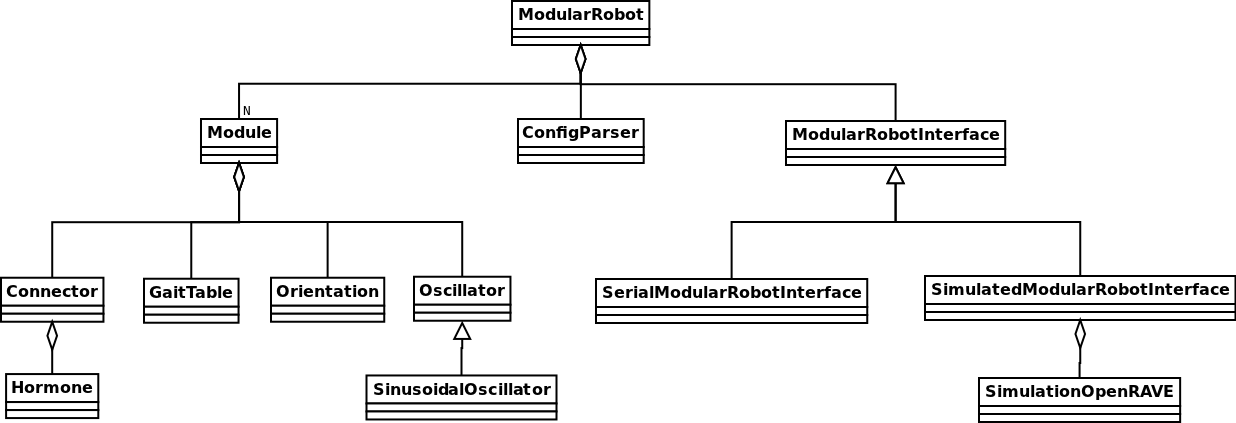
\includegraphics[width=\textwidth]{images/Class_diagram_Main.png}
        \caption{Main class diagram}\label{fig:software_class_main_class}
\end{figure}


Each \emph{Module} has several \emph{GaitTables} to store the parameters of the \emph{SinusoidalOscillator} for the different configurations. At each step of the controller, the \emph{SinusoidalOscillator} class calculates the joint position according to the oscillation. The \emph{SinusoidalOscillator} can be changed by another kind of oscillator thanks to the \emph{Oscillator} interface. The joint angle calculated the \emph{Oscillator} in each \emph{Module} is sent to the robot using a \emph{ModularRobotInterface} interface. \emph{ModularRobotInterface} offers a interface so that several types of robots can be used, either simulated (using the \emph{SimulatedModularRobotInterface}) or real robots communicated through a serial connection (using the \emph{SerialModularRobotInterface}).\\

A \emph{Hormone} class was defined in order to implement the hormone-communication protocol. \emph{Hormones} are sent and received by the any of the four \emph{Connectors} present in each \emph{Module} that model the interconnection of the different modules, allowing the \emph{Hormones} to flow through the modular robot.\\

Finally, the \emph{Orientation} class is a data structure for storing the Tail-Bryan angles (Roll, pitch and yaw) that are obtained by the simulated Inertial Measurement Unit. 


%%%%%%%%%%%%%%%%%% ModularRobot %%%%%%%%%%%%%%%%%%%%%%%%%%%%%%%%%%%%%%%%%%%%%%%%%%%%%%%%%%%%%%%%%%%%%%%%%%%%%%
\subsection{Class ModularRobot}
\label{software_class_modularrobot}

\begin{figure}[h]
		\centering
        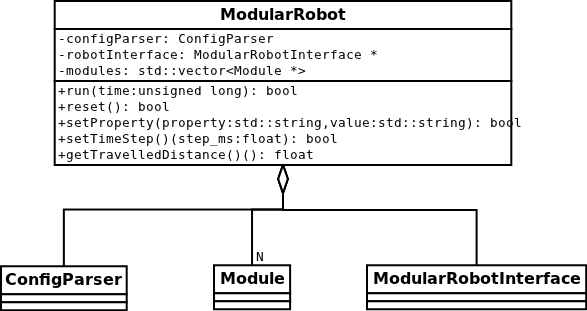
\includegraphics[width=0.6\textwidth]{images/Class_diagram_ModularRobot.png}
        \caption{ModularRobot class diagram}\label{fig:software_class_modularrobot_class}
\end{figure}


\emph{ModularRobot} is the class that encapsulates both the modules and interface with the actual robot (either simulated or real). It counts with several functions that control the robot to perform several operations such as starting or resetting the controllers of all the modules, etc.\\

A \emph{ModularRobot} is constructed using a \emph{ConfigParser} containing the configuration of the modular robot, read from a xml configuration file, which determines the number of modules to be created. A suitable \emph{ModularRobotInterface} is also created, depending on if the robot to be controlled is a real one or a simulation of the modular robot.\\

A series of functions exist to configure the behavior of the \emph{ModularRobot} after the object is created.  The function \emph{setTimeStep()} configures the resolution of the simulation for the simulated robot and the period between packet transmission for the robot controlled by serial port, and using \emph{setProperty()} one can configure other aspects such as enabling/disabling the simulation viewer.\\

After the robot parameters are configured, the module interconnections are read from the \emph{ConfigParser}, and the connectors of the different modules are connected together according to that configuration. This interconnection allows the communication of the different hormones between the modules.\\

Once the robot is configured, and its modules are connected, to start it, the function \emph{run()} is called passing the amount of time, in ms, that the robot will be active. After that amount of time the robot will stop until it receives another call to the \emph{run()} method. Before running again the robot controller, is recommended to make a call to the function \emph{reset()}, to restore the initial configuration, position of the simulated robot, etc.\\

Even though the controller is distributed, and it is supposed to be run in each of the modules independently, the current implementation is simplified to a sequential execution in order to test the hormone-communication protocol in a quick way, so that it can be validated or discarded on an early development stage. Concurrent software is typically difficult to develop and debug, since resources are shared between processes/threads and bugs may appear depending on the order in which those resources where accessed, which causes the appearance of bugs that are difficult of reproduce and fix, since that order is not deterministic. Other common bugs in concurrent software are corruption of data due to simultaneous access to unprotected shared variables or deadlocks ( a process $p_1$ has a lock $l_1$ and it is waiting for another lock, $l_2$, which is held by a process $p_2$ which happens to be waiting for the lock $l_1$).\\

Because of those reasons, the different tasks to be performed by the module controller are implemented as independent member functions, and they are called sequentially for every module before executing the next one. This way a performance similar to the concurrent approach is achieved, but without the increase in development difficulty and time due to concurrent programming. Communications tasks are executed each $T_{comm}$ ms, whereas the joint position is updated each $T_{step}$ ms, allowing to update the joint values more frequently, as the communication tasks can be performed with a larger period, since it is not a time-critical task.\\

Figure \ref{fig:software_class_modularrobot_flowchart} shows the flowchart of the \emph{run()} function of class \emph{ModularRobot}.\\

\begin{figure}[h]
		\centering
        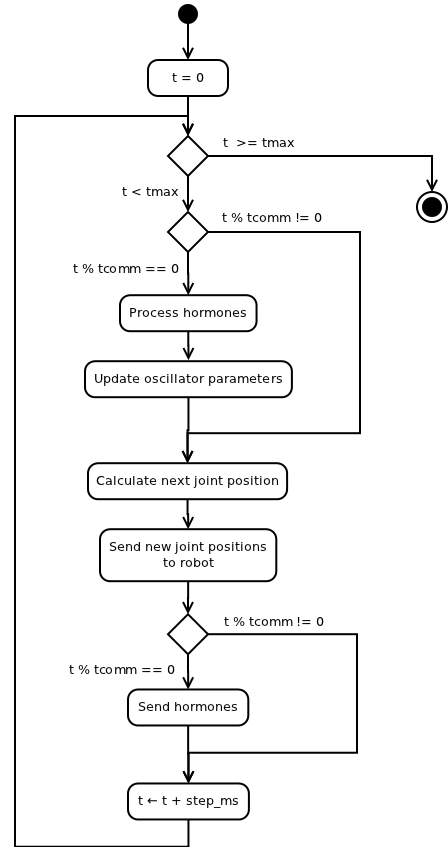
\includegraphics[width=0.4\textwidth]{images/Flowchart_ModularRobot_run.png}
        \caption{ModularRobot::run() flowchart}\label{fig:software_class_modularrobot_flowchart}
\end{figure}

The whole function runs in a loop, repeated until the maximum runtime, $t_{max}$, is reached. Each $t_{comm}$ ms the hormone functions are executed. These functions process the input hormones, obtaining the identifiers for the current module's position, function and global configuration, and setting the required hormones in the output buffers, ready to be sent to the other modules. After the different IDs have been calculated, the oscillator parameters are obtained from the gait tables and set.\\

The next steps, that are executed every $t_{step}$ ms, are the joint values updates. First, the \emph{Oscillator} calculates the new joint value for all the joints at the current time $t$ and, after that, those values are sent to the robot (simulated or real) using the \emph{ModularRobotInterface}.\\

Finally, also each $t_{comm}$ ms, the hormones that were placed on the output buffers are actually sent to the other modules. The time counter is incremented and the loop repeats again until $t_{max}$ seconds have passed.\\

It is important to notice that each of these tasks are executed for each of the modules on the modular robot before moving on to the next task, emulating this way a distributed, concurrent system.\\ 


%%%%%%%%%%%%%%%%%% ConfigParser %%%%%%%%%%%%%%%%%%%%%%%%%%%%%%%%%%%%%%%%%%%%%%%%%%%%%%%%%%%%%%%%%%%%%%%%%%%%%%
\subsection{Class ConfigParser}
\label{software_class_configparser}


\begin{figure}[h]
		\centering
        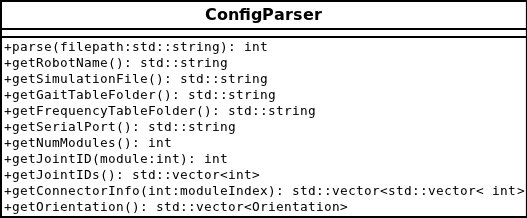
\includegraphics[width=0.6\textwidth]{images/Class_diagram_ConfigParser_members.png}
        \caption{ConfigParser class diagram}\label{fig:software_class_configparser_class}
\end{figure}

Since the \emph{ModularRobot} can be executed with different configurations, it is very convenient to have a way to load those different configurations dynamically without recompiling the whole software. The approach typically followed to achieve this is to use configuration files specifying the different aspects to be configured.\\

For the configuration files, the xml format was chosen, because it is standard, can be read and edited easily by both humans and machines, and there already exist several libraries for parsing xml from different programming languages.\\

The \emph{ConfigParser} class uses one of those libraries, called ``TinyXML2'' to parse the configuration files for the different robot topologies and stores the different parameters loaded in a data structure that can be later accessed by the other components of the project.\\

The tag structure of the configuration files is the following:

\begin{itemize}
	\item All the xml tags of the robot are enclosed on a parent tag called \emph{<ModularRobot>}. This tag has an atribute \emph{``name''} that contains the name of the robot.
\XML
\begin{lstlisting}
<ModularRobot name="TestRobot">
	
    <!-- Robot config goes here -->
	
</ModularRobot>
\end{lstlisting}
	
	\item Inside \emph{<ModularRobot>} go the global configuration parameters and the definition of the different modules. The global parameters to be configured are: the path to the openRAVE xml model of the robot for the simulation, with the tag \emph{<simulationFile>}; the path to the folder containing the gait tables, with the tag \emph{<gaitTableFolder>} and the path to the file with the table containing the frequencies of the oscillators for the different configurations, \emph{<frequencyTable>}. The serial port used to communicate with the real robot is configured in the tag \emph{<serialPort>}.
	
\newpage
\XML
\begin{lstlisting}
<ModularRobot name="TestRobot">

    <simulationFile>../../data/models/REPY-2.1/MultiDof-7-tripod.env.xml</simulationFile>
    <gaitTableFolder>../../data/gait tables/</gaitTableFolder>
    <frequencyTable>../../data/gait tables/frequencies.txt</frequencyTable>
    <serialPort>/dev/ttyUSB0</serialPort>
	
    <!-- Rest of the configuration goes here -->
	
</ModularRobot>
\end{lstlisting}
	
	\item Modules are defined after that, using the tag \emph{<Module>}. Inside this tag, the different parameters of the module are to be set, such as the joint index ( set with \emph{<Joint>}), the initial orientation of the module and the different connections between modules.
	
	The initial orientation defined in the configuration file under the tag \emph{<Orientation>}  is the one the module takes as if it were the readings of the Inertial Measurement Unit, emulating this piece of hardware that the current module version lacks. The different values for the angles are set in the tags \emph{<Roll>}, \emph{<Pitch>} and \emph{<Yaw>}, respectively.\\
	
	Connections between modules are set under the tag \emph{<Connections>}. Each of the local connectors (front, right, back and left) has its own tag for setting the parameters of that connector. Those parameters are atributes of the corresponding tag, such as \emph{connectedTo}, indicating which module is the current connector connected to; \emph{connector}, which represents the index of the remote connector that is connected to the current connector (0 for front, 1 for right, 2 for back and 3 for left) and  \emph{orientation}, which represents the relative orientation of the connectors, and that currently it is only used for debugging and testing purposes.

	Here we have an example of a complete xml robot configuration file for a simple 2-module configuration:
	\XML
\begin{lstlisting}
<ModularRobot name="TestRobot">
    <simulationFile>../../data/models/REPY-2.1/Kusanagi-2.env.xml</simulationFile>
    <gaitTableFolder>../../data/gait tables/</gaitTableFolder>
    <frequencyTable>../../data/gait tables/frequencies.txt</frequencyTable>
    <serialPort>/dev/ttyUSB0</serialPort>  	
    <Module>
        <Joint>0</Joint>		
        <Connections>
            <front connectedTo="1" connector="Back" orientation="0"></front>
        </Connections>
        <Orientation>
            <Roll>0</Roll>
            <Pitch>0</Pitch>
            <Yaw>0</Yaw>
        </Orientation>
    </Module>
    <Module>
        <Joint>1</Joint>
        <Connections>
           <back connectedTo="0" connector="Front" orientation="0"></back>
         </Connections>
        <Orientation>
           <Roll>0</Roll>
           <Pitch>0</Pitch>
           <Yaw>0</Yaw>
        </Orientation>
    <Module>
</ModularRobot>
\end{lstlisting}
	
\end{itemize}

\newpage

%%%%%%%%%%%%%%%%%% ModularRobotInterface %%%%%%%%%%%%%%%%%%%%%%%%%%%%%%%%%%%%%%%%%%%%%%%%%%%%%%%%%%%%%%%%%%%%
\subsection{Class ModularRobotInterface}
\label{software_class_modularrobotinterface}

\begin{figure}[h]
		\centering
        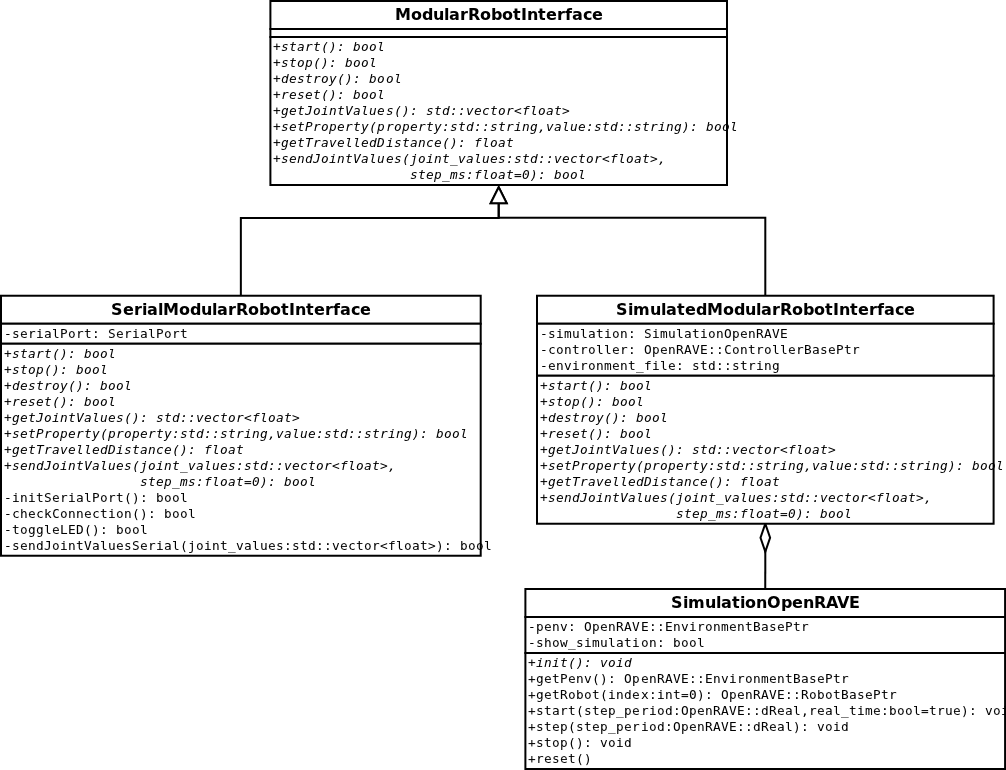
\includegraphics[width=0.9\textwidth]{images/Class_diagram_ModularRobotInterface.png}
        \caption{ModularRobotInterface class diagram}\label{fig:software_class_modularorobotinterface_class}
\end{figure}

Although the controller is distributed, the modular robot used to test the gait has a central controller, due to hardware limitations of the modules used in this work. For that reason, the \emph{ModularRobot} class owns a interface with the modular robot, in order to send commands to it, so that it can set the joints of the robot to the desired values or, in the future, receive sensor data from the robot, to implement more complex controllers.\\

The class \emph{ModularRobotInterface} acts as a bridge between the controller, being run on the computer, and the robot. As the robot to be controlled can be either a simulated one, for gait discovery and testing or the physical one, to verify that the gaits work on the real worl, this class is an abstact class that act defining the interface in a computer science sense, that is, the functions that the classes that follow this interface must define. This way, the different interfaces for the different types of robot can be used indistinctly by the modular robot controller, just having to change which class is instantiated to change the behaviour of the program.\\

Two different classes have been implemented following the \emph{``ModularRobotInterface''} ~interface:
\begin{itemize}
	\item \emph{SimulatedModularRobotInterface}, to control the modular robot simulated on openRAVE.
	\item \emph{SerialModularRobotInterface}, that controls the physical robot via the  computer serial port.
\end{itemize}
Instances of those clases are created using a factory method pattern, a function that generates objects that follow a certain interface without needing to specify the exact class of object that will be created.\\

The interface has four main functions to implement for the initialization and destruction of the interface, one for the setup of certain properties or variables, and three for the control of the robot. The purpose of each of the function is the following:

\begin{itemize}
	\item bool \emph{start()}: this function is used for the initialization of the robot interface, for example, to start the simulation or to connect to the robot with the serial port.
	
	\item bool \emph{stop()}: with this funtion the robot interface is stopped. This can be used, for instance, to stop the simulation or to interrupt the communication via serial port.
	
	\item bool \emph{destroy()}: this function is meant to be called in order to free all the dynamically allocated memory and to do all the required steps in order to destroy the object.
	
	\item bool \emph{reset()}: used to reset the interface, for example, restarting the simulation or the serial connection.
	
	\item bool \emph{setProperty(} std::string property, std::string value\emph{)}: this function should be used to configure the different properties or parameters of the interface. The string property specifies which is the property to modify, and the string value contains the new value for that parameter. This can be used, for example, to specify if the simulator viewer is to be visible or not.
	
	\item bool \emph{getTravelledDistance()}: returns the distance travelled by the robot. The method used for calculating this distance depends on the implementation of the robot interface.
	
	\item bool \emph{sendJointValues(} std::vector<float> joint\_values, float step\_ms = 0\emph{)}: sends the desired joint values to the robot. The step\_ms parameter can be used to specify the amount of time to wait for the joints to reach the position, in order to run the simulation for the time of that step, for example.
	
	\item std::vector<float> \emph{getJointValues()}: returns all the joint positions stored in a vector.
\end{itemize}

%%%%%%%%%%%%%%%%% SIMULATED ROBOT INTERFACE %%%%%%%%%%%%%%%%%%%%%%
\subsection{Class SimulatedModularRobotInterface}
\label{software_class_simulatedmodularrobotinterface}

This class implements the \emph{ModularRobotInterface} interface, and it is used to start a simulation and control the simulated robot. For that purpose it uses a \emph{SimulationOpenRAVE} objects that encapsulates all the details of starting a OpenRAVE simulation and controlling it. \\

If the simulation is to be run continously, it can be started with the \emph{start()} function. If not, the simulation is run step by step, with the step time specified in the \emph{sendJointValues()} method. The \emph{stop()} and \emph{reset()} methods stop and restart the OpenRAVE simulation and with the \emph{destroy()} method the memory for the simulation object can be freed.\\

The user can decide whether or not the simulation viewer is enabled by calling the \emph{setProperty()} method with the property ``viewer'' and the value ``enabled''.\\

For the travelled distance calculation, the initial position of the robot is stored at the start of the simulation, and when the function \emph{getTravelledDistance()} is called, that distance is calculated by computing the distance between that initial point and the current position. Calculated this way, the distance is always less than actual distance travelled, unless the robot moves in a straight line, which favors that the gaits resulting from the evolutionary algorithm follow a straight line, as this way the fitness value (average speed) is greater. \\

The joint values are accessed directly through a reference to the OpenRAVE Controller that is set on the robot, both for sending the new joint values, or to read the current ones. A step time can be specified, so that the simulation is advanced that amount of time for the joints to have time to move to their desired positions.\\

%%%%%%%%%%%%%%%%% SIMULATION OPENRAVE %%%%%%%%%%%%%%%%%%%%%%%%%%%%%%
\subsection{Class SimulationOpenRAVE}
\label{software_class_SimulationOpenRAVE}

In this work, OpenRAVE has been chosen as simulator, but many others exist. Having a class for encapsulating the simulation allows not only to add support to different simulators in the future, but also to offer a simple and generic interface for interacting with the simulation.\\

The \emph{SimulationOpenRAVE} class offers a control interface similar to the \emph{ModularRobotInterface} one, with functions for starting, stopping and resetting the simulation. It has also a function \emph{step()} to run the simulation step by step, instead of running it continuously.\\

It creates a OpenRAVE simulation, loads the environment with the modular robot to be simulated, sets the Servocontroller from the OpenMR plugin for controlling all the joints, gets references to the environment and robots, which can be later obtain with the \emph{getPenv()} and \emph{getRobot()} methods.\\

The viewer offered by OpenRAVE can be enabled either when creating the \emph{SimulationOpenRAVE} object or later, calling the \emph{showViewer()} method.\\

%%%%%%%%%%%%%%%%% SERIAL ROBOT INTERFACE %%%%%%%%%%%%%%%%%%%%%%
\subsubsection{Class SerialModularRobotInterface}
\label{software_class_serialmodularrobotinterface}

The \emph{SerialModularRobotInferface} class implements the \emph{ModularRobotInterface}, and it is used to send the joint values to the real robot through a serial connection.\\

When the \emph{start()} method is called, the serial port is open and the program connects with the modular robot until the communication is interrupted by calling \emph{stop()} or \emph{reset()}. Once the communication is halted, the allocated memory can be freed by calling the \emph{destroy()} method.\\

The joint values are sent to the robot using the function \emph{sendJointValues()}, which internally converts the values from the range of the oscillator ($[-90,90]$) to the range of the hardware servos ($[0,180]$) before sending them through the serial port. Since the robot does not count with any means of measuring the actual joint position, the sent values are stored in the \emph{SerialModularRobotInferface}, and can be requested by the user calling the \emph{getJointValues()} method.\\

Since the modular robot currently cannot sense its actual position (using internal measurements or with computer vision employing an external camera), the \emph{getTravelledDistance()} method just outputs a warning explaining that the distance travelled measurement is not implemented yet.\\

Finally, since the controller board has a LED available for visual signaling, a property called ``LED'' with a value ``toggle'' can be set to the \emph{SerialModularRobotInferface} using the \emph{setProperty()} method to turn it on and off.\\


%%%%%%%%%%%%%%%%%% Module %%%%%%%%%%%%%%%%%%%%%%%%%%%%%%%%%%%%%%%%%%%%%%%%%%%%%%%%%%%%%%%%%%%%
\subsection{Class Module}
\label{software_class_module}

\begin{figure}[h]
		\centering
        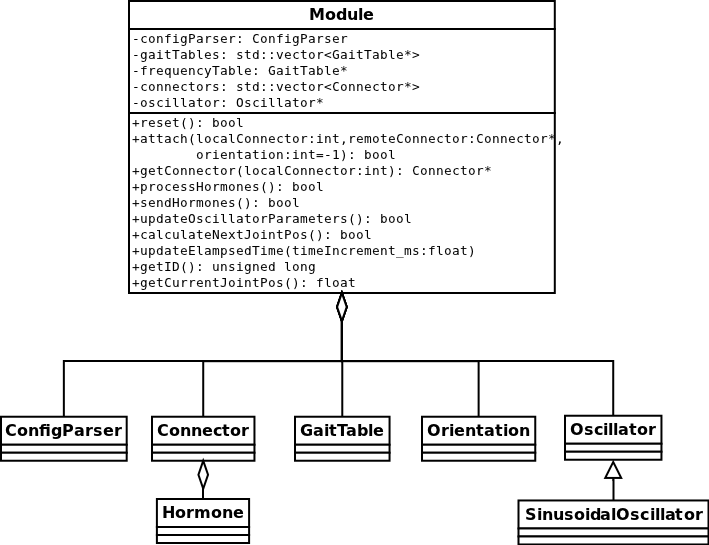
\includegraphics[width=0.6\textwidth]{images/Class_diagram_Module.png}
        \caption{Module class diagram}\label{fig:software_class_module_class}
\end{figure}

The class \emph{Module} represents the controller of each of the modules. This controller is homogeneous for the whole modular robot, each module is an instance of the same Module class.\\

A \emph{ConfigParser} is passed to the constructor with the parameters read from the configuration file, as well as the index of the module to be created, so that the correct parameters are extracted from the \emph{ConfigParser}.\\

For generating the oscillations, the \emph{Module} class has a \emph{Oscillator} object, that updates the joint position of the module. For this thesis the oscillators used are \emph{SinusoidalOscillator}, but as the \emph{Oscillator} class defines a interface for oscillators, new kinds of different oscillators can be added very easily to the project, and used without changing the code for the \emph{Module} controller.\\

The parameters for the oscillator are stored on several \emph{GaitTables}, one for the main parameters (amplitude, offset and phase) for each of the three configurations discussed on this work, and a extra one for the different frequencies for each configuration. These parameters are accessed using the IDs obtained through the hormone communication protocol. How to calculate those IDs is explained on section \ref{config_repy_description}, and the hormone communication protocol is presented on chapter \ref{hormones}.\\

One of the required data for calculating the IDs is the initial orientation of the module. There exists a class in this project, called \emph{Orientation}, that stores the data for the orientation angles. It has also several functions to do simple operations with \emph{Orientations}, as well as a function that calculates the relative orientation between the orientations of two modules, a piece of data that is key to the ID calculation.\\

For the interconnection of modules, and their communication, a class \emph{Connector} was implemented. There are 4 connectors on each module, and each \emph{Connector} has an input buffer and an output buffer to store the incoming and outgoing \emph{Hormones}, and a reference pointing to the remote \emph{Connector} they are attached to. The \emph{Hormone} class models the different types of hormones used in the hormone communication protocol, to be explained in chapter \ref{hormones}.\\ 

In order to emulate the distributed controller from a sequential approach, so that the software can be developed and validated in a faster way, the controller of the module is split in several small tasks, that are executed for all the modules before starting the next one.\\

The first task to be executed is the hormone processing. Hormones are recovered from the connectors' input buffers and processed depending on their type, as explained in section \ref{hormone_algorithm}. ``Ping'' hormones are processed first, obtaining from them the ID related to the position of the module inside the modular robot.  Then, the ``Leg'' hormones are either processed or generated in case of the ``leg'' modules. From the ``Leg'' hormones the ``head'' module will discover which is the global configuration of the robot and will generate ``Head'' hormones. Finally, if the module is not the ``head'' module,  those ``Head'' hormones are processed, obtaining the configuration ID obtained by the ``head'' module. Generated hormones are put in the output buffer in this task, ready to be sent to the connected modules.\\

Once the IDs are obtained, the next task to be performed consists in querying the new oscillator parameters to the corresponding gait tables, and setting them on the oscillator. With the ID of the current configuration the corresponding gait table for the amplitude, offset and phase of the oscillators is selected, and using the ID related to the function inside the modular robot global configuration the suitable parameters are obtained from the table and set on the oscillator. This task, as well as the previous one, are executed periodically at a different rate than the joint position update, with a period of $t_{comm}$ milliseconds.\\

After that, the oscillator will update the joint value for the module, calling \emph{calculateNextJoinPos()} with the elapsed time as parameter. The modular robot will recover this joint position value, put it in a vector with the other modules' joint values and send them to the \emph{ModularRobotInterface}.\\

Finally, the hormones stored in the output buffers will be sent to their destination modules, and the local elapsed time of the module will be updated.\\


%%%%%%%%%%%%%%% Oscillator %%%%%%%%%%%%%%%%%%%%%%%%%%%%%%%%%%%%%%%%%
\subsection{Class Oscillator}
\label{software_class_oscillator}

In order to generate the oscillations that drive the joints of the modular robot in order to achieve locomotion, the \emph{Oscillator} class is employed. This class is designed as an abstract class that stores the main oscillator parameters, and lefts the actual implementation of the oscillator to the classes that implement this interface. This way, the module controller can work with several types of oscillators without changing the controller code, just switching the \emph{Oscillator} class used.\\

The calculation of the joint position from the elapsed time is performed on the function \emph{calculatePos()}, which has to be implemented in the classes that follow the \emph{Oscillator} interface.\\
\begin{figure}[h]
		\centering
        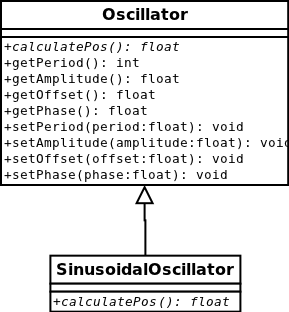
\includegraphics[width=0.3\textwidth]{images/Class_diagram_Oscillator.png}
        \caption{Oscillator class diagram}\label{fig:software_class_oscillator_class}
\end{figure}


\subsection{Class SinusoidalOscillator}
\label{software_class_sinusoidaloscillator}

The only type of \emph{Oscillator} implemented in this project is the \emph{SinusoidalOscillator}, which models the joint position values as an oscillating sinewave.\\

The \emph{calculatePos()} method calculates the position following a sinusoidal function, characterized by the amplitude, offset, phase and period stored on the \emph{Oscillator} base class. Using the elapsed time, the joint position is calculated the following way:
\begin{equation} \label{eq:software_sinusoidal_oscillator}
\varphi(t) = A_i \cdot \sin{\left( \frac{2\pi}{T} \cdot t + \Phi_i \right)} + O_i
\end{equation}\\

Sinusoidal oscillators are explained in more detail on section \ref{gait_sin_osc}.

%%%%%%%%%%%%%%% Connector   %%%%%%%%%%%%%%%%%%%%%%%%%%%%%%%%%%%%%%%%%
\subsection{Class Connector}
\label{software_class_connector}

\begin{figure}[h]
		\centering
        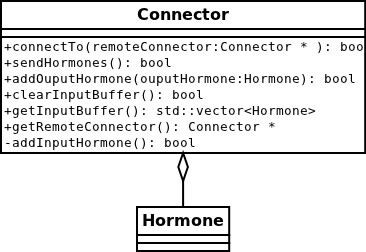
\includegraphics[width=0.3\textwidth]{images/Class_diagram_Connector.png}
        \caption{Connector class diagram}\label{fig:software_class_connector_class}
\end{figure}


In order to model the different connectors that allow the modules to be attached to other modules, the \emph{Connector} class is used.\\

The \emph{Connector} class is a simple data container that has two buffers, one for storing the incoming hormones prior to their processing, and other for placing the outgoing hormones before they are actually sent to the remote connector attached to this connector.\\

This class also contains a reference to the remote \emph{Connector} attached to this connector, in order to be able to send the hormones from the ouput buffer. This reference is set with the \emph{connectTo()} method.\\

For sending out the hormones in the output buffer to the remote module input buffer, the method \emph{sendHormones()} is used, which takes the hormones stored in the ouput buffer and puts them in the input buffer of the remote module using the reference to that module and the \emph{addInputHormone()} function.\\

The \emph{localOrientation} attribute contains the relative orientation between the local and remote modules calculated by hand. This attribute is no longer in use by the controller, which currently calculates it from the orientation of both modules, dynamically.\\


\subsection{Class Hormone}
\label{software_class_hormone}

\begin{figure}[h]
		\centering
        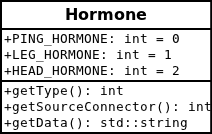
\includegraphics[width=0.2\textwidth]{images/Class_diagram_Hormone_members.png}
        \caption{Hormone class diagram}\label{fig:software_class_hormone_class}
\end{figure}

The \emph{Hormone} class is the base for the hormone communication protocol, one of the key aspects of this work. The class is a container for the info that is needed to be transmitted to the other modules.\\

A \emph{Hormone} has 3 fields: the type of hormone (``Ping'', ``Leg'' or  ``Head''), encoded as an integer; the connector that sent the hormone, also encoded as integer (0, 1, 2 and 3 for the front, right, back and left connectors, respectively) and a data field to attach extra info required for the modules to discover the IDs.\\

The contents of the data field depend on the type of hormone. ``Ping'' hormones store in the data field the local orientation of the module that sends the hormone as a string (i.e. ``90 180 270'', meaning roll=90º, pitch=180º and yaw=270º). ``Leg'' hormones do not need any extra info, so their data field is empty, and ``Head'' hormones store in the data field the ID of the global configuration as discovered by the ``head'' module ( 0 for \emph{MultiDof-11-2}, 1 for \emph{MultiDof-7-tripod} or 2 for  \emph{MultiDof-9-quad}) and, if needed, an extra integer for leg dissambiguation.\\

The hormone communication protocol is explained in detail on chapter \ref{hormones}.\\

\newpage

\subsection{Class GaitTable}
\label{software_class_gaittable}

\begin{figure}[h]
		\centering
        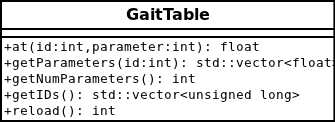
\includegraphics[width=0.3\textwidth]{images/Class_diagram_GaitTable_members.png}
        \caption{GaitTable class diagram}\label{fig:software_class_gaittable_class}
\end{figure}

The class \emph{GaitTable} stores the oscillator parameters relating them to a ID. The data is stored as a table, with the different parameters for each ID stored as rows of the table. An example of the internal representation of a gait table for the main oscillator parameters is shown in table \ref{table:gait_table_example}. 

\begin{table}[h]
\centering
\begin{tabular}{|c||c|c|c|} \hline
 ID & Amplitude & Offset & Phase \\ \hline \hline
83506 & 60 & 0 & 0 \\ \hline
78896 & 60 & 0 & 120 \\ \hline 
\end{tabular}
\caption{Example of the internal contents of a gait table for a 2 module configuration}
\label{table:gait_table_example}
\end{table}

The \emph{GaitTable} can receive queries for a given ID, and then it returns all the parameters corresponding to that ID. The data is stored and read using text files, in a format that is compatible with the Matlab/Octave text file format.\\

\subsection{Class Orientation}
\label{software_class_orientation}


\begin{figure}[h]
		\centering
        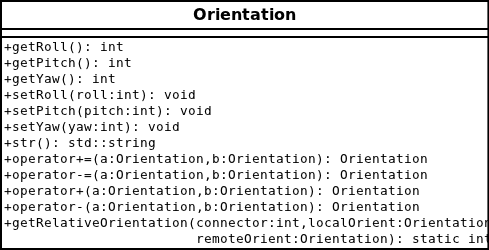
\includegraphics[width=0.45\textwidth]{images/Class_diagram_Orientation.png}
        \caption{Orientation class diagram}\label{fig:software_class_orientation_class}
\end{figure}

For calculating the ID based on the position of the module inside the modular robot, a module needs to know the relative orientation between the attached connectors. To work with those Orientations, the class \emph{Orientation} was implemented. \emph{Orientation} is supposed to be measured by the module with a Inertial Measuremente Unit (IMU) but, as the modules do not have a IMU because of hardware limitations, the IMU is currently simulated by reading the initial values that the IMU would return from the robot configuration file.\\

For expressing the orientation, we are using Tait-Bryan angles, a representation largely used in aeronautics, and the one that the IMU returns by default. This representation, similar to the Euler Angles, expresses the orientation of an object with three angles: roll, pitch and yaw. These angles represent rotations around the three main axes of a fixed reference frame, roll corresponding to the rotation around the Z axis; pitch being a rotation about the Y axis and finally yaw, a rotation about the X axis. Notice that, unlike Euler Angles, these rotations are performed around a reference frame that is fixed in the world, not in the object, and therefore it does not rotate with the object.\\
\begin{figure}[h]
		\centering
        \begin{subfigure}[b]{0.4\textwidth}
                \centering
                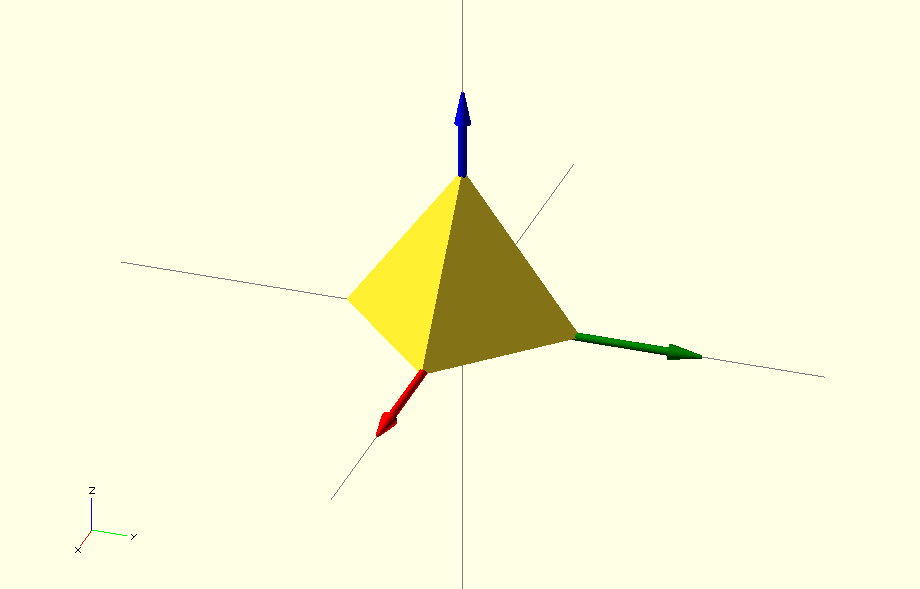
\includegraphics[width=\textwidth]{images/Orientation/tait-bryan-01.png}
                \caption{Initial orientation}
                \label{fig:soft_orientation_initial}
        \end{subfigure}
        ~
        \begin{subfigure}[b]{0.4\textwidth}
                \centering
                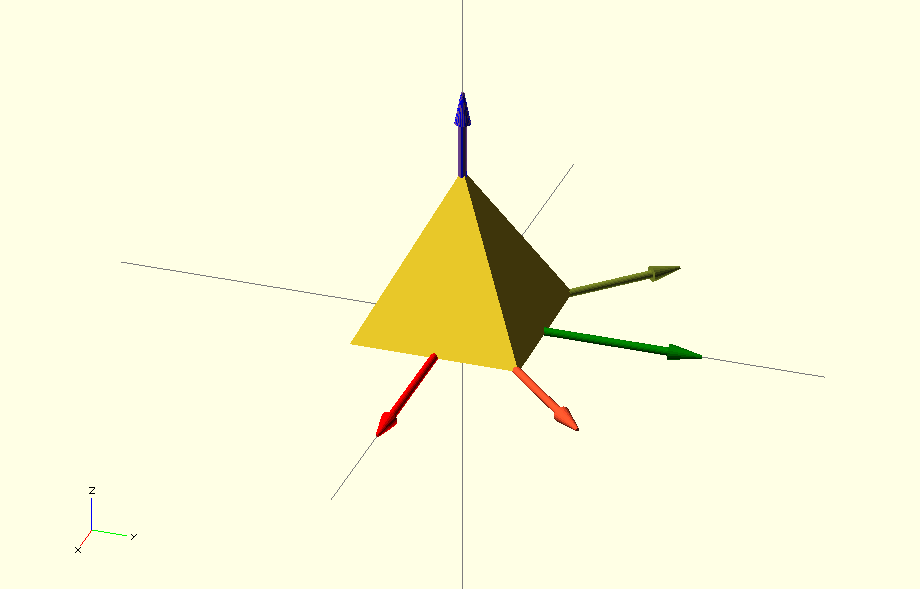
\includegraphics[width=\textwidth]{images/Orientation/tait-bryan-02.png}
                \caption{Roll 45º around Z axis }
                \label{fig:soft_orientation_roll}
        \end{subfigure}
        ~
        \begin{subfigure}[b]{0.4\textwidth}
         	   \centering
                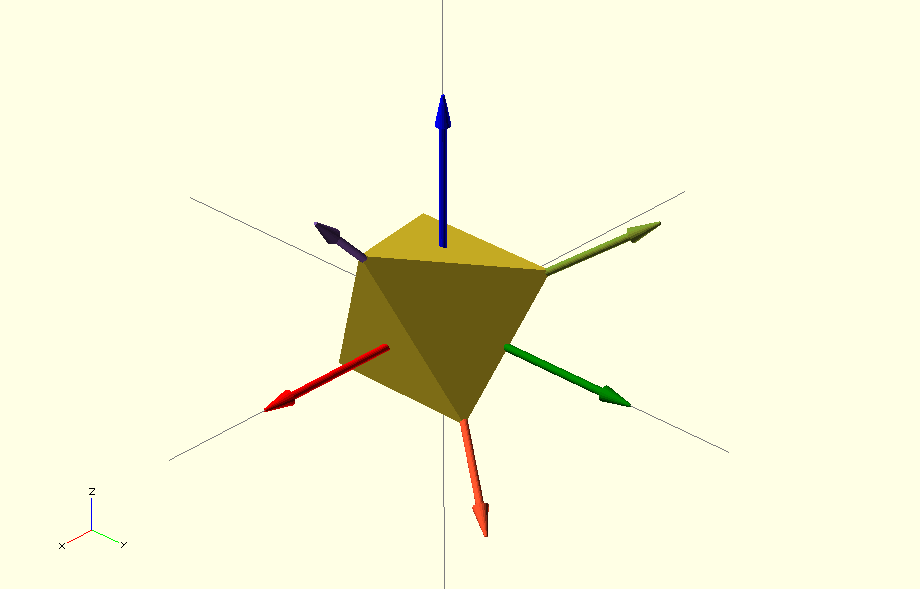
\includegraphics[width=\textwidth]{images/Orientation/tait-bryan-03.png}
                \caption{Pitch 45º around Y axis}
                \label{fig:soft_orientation_pitch}
        \end{subfigure}        
        ~
        \begin{subfigure}[b]{0.4\textwidth}
         	   \centering
                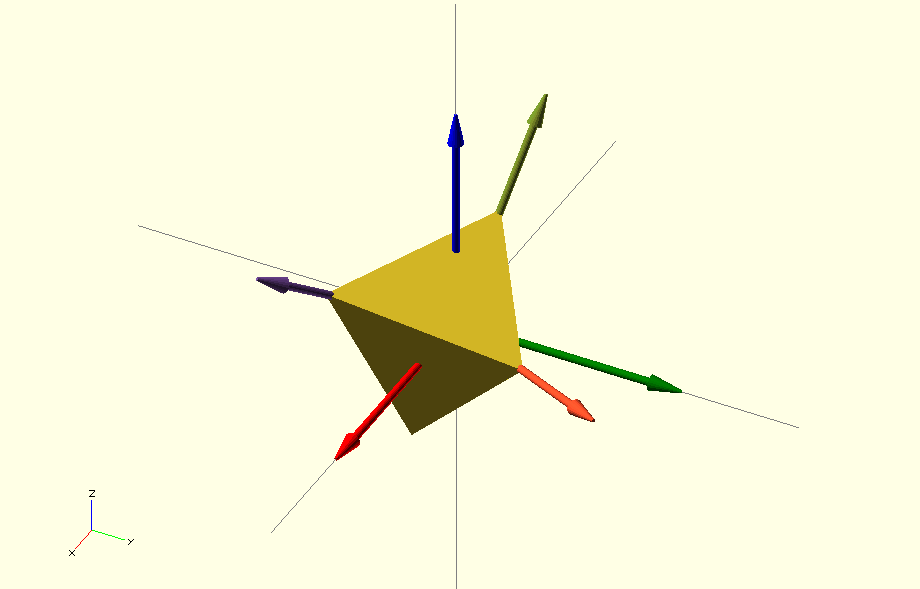
\includegraphics[width=\textwidth]{images/Orientation/tait-bryan-04.png}
                \caption{Yaw 45º around X axis}
                \label{fig:soft_orientation_yaw}
        \end{subfigure}
        \caption{Steps to obtain a pyramid with a orientation of (45º, 45º, 45º) expressed in Tait-Brian angles RPY}\label{fig:soft_orientation_example}
\end{figure}


Inside the \emph{Orientation} class, angles are bound to the interval [0, 360), and the class counts with several functions to perform simple arithmetic operations with them, as well as to convert them to a string for storing the \emph{Orientation} on the data field of the \emph{Hormone} class. For calculating the relative rotation between two modules, the function \emph{getRelativeOrientation} can be used, passing it the ID of the connector that is used as reference (0, 1, 2 and 3 for front, right, back and left, respectively) as well as the local and remote module orientations.\\

The relative rotation between two modules is expressed as an integer value from 0 to 3 that represents the number of 90º steps we have to rotate the local module around the axis of the local reference system that is in the same direction as the normal vector of the local connector surface, such as the Z axis of the local reference system of both modules coincide. This is explained in more detail, with graphical examples in section \ref{config_repy_description}.\\

The algorithm used by \emph{getRelativeOrientation()} to calculate the relative rotation value is the following:

\begin{enumerate}
	 \item Roll, pitch and yaw angles are equivalent to Euler XYZ angles, so we use this property to calculate the transformation matrices for both reference systems (the one from the local module and the one from the remote module) by multiplying the rotation matrices around X (yaw), Y (pitch) and Z (roll).
	 \[ ^{0}H_A = Rot_X(\gamma_A) * Rot_Y(\beta_A) * Rot_Z(\alpha_A) \]
	 \[ ^{0}H_B = Rot_X(\gamma_B) * Rot_Y(\beta_B) * Rot_Z(\alpha_B) \]
	 
	 Were $~^{0}H_{x}$ is the homogeneous transformation matrix to go from the absolute reference system to x, A is the local module reference system, B is the remote module reference system and $\alpha$, $\beta$ and $\gamma$ are roll, pitch and yaw angles, respectively. In a matricial form, the previous equations become:
	 
	 \[  ^{0}H_A =  
	 \begin{bmatrix}
	 1 & 0 & 0 \\ 
	 0 & \cos(\gamma_A) & -\sin(\gamma_A)\\
	 0 & \sin(\gamma_A) & \cos(\gamma_A)
	 \end{bmatrix}
	 \begin{bmatrix}
	 \cos(\beta_A)  & 0 & \sin(\beta_A) \\ 
	 			0   & 1 & 			0  \\
	 -\sin(\beta_A) & 0 & \cos(\beta_A)
	 \end{bmatrix}
	 	 \begin{bmatrix}
	  \cos(\alpha_A)  & -\sin(\alpha_A) & 0 \\ 
	  \sin(\alpha_A)  &  \cos(\alpha_A) & 0 \\
	 			   0  &               0 & 1
	 \end{bmatrix}\]	 	 
	 \[  ^{0}H_B =  
	 \begin{bmatrix}
	 1 & 0 & 0 \\ 
	 0 & \cos(\gamma_B) & -\sin(\gamma_B)\\
	 0 & \sin(\gamma_B) & \cos(\gamma_B)
	 \end{bmatrix}
	 \begin{bmatrix}
	 \cos(\beta_B)  & 0 & \sin(\beta_B) \\ 
	 			0   & 1 & 			0  \\
	 -\sin(\beta_B) & 0 & \cos(\beta_B)
	 \end{bmatrix}
	 	 \begin{bmatrix}
	  \cos(\alpha_B)  & -\sin(\alpha_B) & 0 \\ 
	  \sin(\alpha_B)  &  \cos(\alpha_B) & 0 \\
	 			   0  &               0 & 1
	 \end{bmatrix}\]\\
	 
	 \item We undo the rotation of the local module reference system to make it coincide with the absolute reference frame, and apply the same inverse transformation to the remote module reference system, obtaining the homogeneous tranformation matrix to go from A (local module) to B (remote module):
	 \[  ^{A}H_B = ~^{A}H_0 \cdot ~^{0}H_B = (~^{A}H_0)^{-1} \cdot ~^{0}H_B  \]
	 
	 \item We find the Z vector of the remote reference system ($ \vec{k'}$) by multiplying the unit Z vector of the absolute reference system ($ \vec{k}$) by the homogeneous tranformation matrix.
	 \[ \vec{k'} = ~^{A}H_B ~ \vec{k} = ~^{A}H_B \begin{bmatrix} 0\\ 0\\ 1 \end{bmatrix}\]
	 
	 \item Iteratively, the vector $\vec{k}$ is rotated in steps of 90º until it matches with the vector $\vec{k'}$ calculated in the previous step. The axis of rotation depends on which is the connector of the local module being evaluated, for the front and back connectors, the Y axis is used, whereas for the left and right connectors, it is the X axis. The number of steps required to match them is the relative rotation value returned by the function.
\end{enumerate}


%%%%%%%% EXECUTABLES %%%%%%%%%%%%%%%%%%%%%%%%%%%%%%%%%%%%%%%%%%%%%%%%%%%%%%%%%%
\section{Applications}
\label{software_apps}

Apart from the main framework, the Hormodular software has several applications to perform the optimization of the locomotion parameters and their evaluation either on the simulated robot, or the real robot via serial port. The source code for these applications can be found in the ``src/apps'' folder inside the project main directory and, once compiled, these applications can be found in the ``bin'' folder.

\subsection{evolve-gaits}
\label{software_evolve-gaits}
The program ``evolve-gaits'' is used for finding the best oscillator parameters in order to achieve an optimal gait on a given modular robot configuration. This program uses the Evolutionary Computing Framework (ECF) library to perform the optimization of those parameters using the Differential Evolution algorithm (Described on section \ref{evolution_algorithm}). For the evaluation of the gait generated by the oscillator parameters of an individual of the Differential Evolution population we implemented a very simple controller that just performs the joint position update according to the joint values provided by the sinusoidal oscillators with the parameters to be evaluated.\\

The usage of the program is not complex, as it only takes an argument for its execution, the evolution configuration file. The configuration file is a xml file containing a set of tags defined by the authors of the ECF library in order to configure the optimization algorithm. Some of the parameters that can be configured with this file are: the type of optimization algorithm and its parameters, the type of genotype to be used, the population size and the number of iterations, among others. ECF also allows the users of the library to define custom tags to configure other aspects of the evolution, such as the path of the robot configuration file, the evaluation time of the robot gait, or the limits of the sinusoidal oscillator parameters.\\

The program will read this parameters and it will execute the optimization algorithm. A log file is configured to be automatically created to track the progress of the algorithm, and a milestone file is generated with data that can be used to resume the execution of the evolution in case the program crashes or is interrupted. This milestone file also contains the genotype of the best individual, from we will extract the oscillator parameters for the best gait.\\

These parameters are encoded in the genotype with normalized values in the interval $[-1, 1]$ due to limitations of the ECF that do not allow to set different value limits for different parameters of a single genotype. To obtain the non-normalized values without doing operations by hand, and set them on a gait table, a Octave/Matlab simple script was developed, and can be found in the ``Utils'' folder that will generate the required data from the normalized values returned by the evolution program.\\


\subsection{evaluate-gaits-sim}
\label{software_evaluate-gaits-sim}
Once the best parameters have been found, we would want to evaluate those parameters, as well as the hormone communication protocol, in order to check if a suitable gait was found, and if the hormone controller performs as desired. In order to test it on the simulated robot, the ``evaluate-gaits-sim'' application can be used.\\

This program just creates a \emph{ModularRobot} instance with a simulated \emph{ModularRobotInterface} and configures it with the parameters specified by the user. Then, it runs the simulation for the specified run time and reports the results of the evaluation to the user. The resulting gaits can be observed on the simulation viwer offered by OpenRAVE.\\

The usage of this program is simple. It requires the user to call the program specifying the xml robot configuration file and the time the robot will be simulated (simulation time), with an optional parameter being the simulation step time, which  is 0.25 ms by default. At the end of the evaluation, the program shows the real time that it took to simulate the robot during the run time specified by the user, as well as the distance travelled by the robot.\\


\subsection{evaluate-gaits-serial}
\label{software_evaluate-gaits-serial}
Since the final objective is to control a real modular robot with the controller, it is very useful to test the gaits and the hormone controller on the real modular robot. For that purpose the ``evaluate-gaits-serial'' program exists.\\

This program creates a \emph{ModularRobot} with a \emph{SerialModularRobotInterface}, connecting with the robot through the serial port and sending it the commands required to drive the servos to the desired positions. The modular robot, in the current state of development acts as a ``dummy'' robot: the distributed controller for each of the modules runs on the computer, and it sends to the robot the position of the different joints, which allows the robot to move, and allow us to test if the gaits are effective and optimal in a real-world environment.\\

The parameters for running the ``evaluate-gaits-serial'' program are exactly the same as the ones for the simulated robot evaluation, but in this case the step time corresponds to the rate of update of the robot joints, which has been increased to 2 ms by default due to bandwidth limitations of the serial port.\\


\subsection{Utils}
\label{software_utils}

Apart from the main programs, the repository includes a series of scripts that solve in a fast way some of the repetitive and dull tasks that appear during the development process.\\

The first one is a Python script called \emph{IDcalculator.py}, that takes a string containing the connection description in a human-readable way as argument and translates it to the actual ID number. An example of its usage would be:
\Bash
\begin{lstlisting}
  $ python IDcalculator.py "((L,90), X, (R, 270), X)"
\end{lstlisting}
%$

In which each of the four elements of the top level 4-tuple is the information of the remote connector connected to the front, left, right and back connector, respectively, with `X' denoting that there is nothing connected to that connector. The elements of the inner tuples are the remote connector attached to the local connector, and coded with the initial of that connector (i.e. L for left or R for right) and the relative orientation between connectors. In the example above, that ID would correspond to a module with the left connector of another module attached to the front connector at an relative angle of 90º, and the right connector of other module attached to the back connector at a relative angle of 270º which corresponds to the ID 82644.\\

The second one is a Octave/Matlab script called \emph{vectorToTable.m} that converts a vector containing the genotype resultant from the optimization process to a gait table. This genotype contains the optimized oscillator parameters normalized in the interval $[-1,1]$. The parameter limits are specified when calling the function defined in the script, returning a table with the parameters already scaled back to the non-normalized form. If we want to obtain the gait table for a \emph{MultiDof-9-tripod} configuration, optimized with $A_{max} = 80º$,  $O_{max} = 45º$, $\phi_{max} = 360º$ and $f_{max} = 1.5Hz$, the function would be called as follows:

\Bash
\begin{lstlisting}
  $ octave
  
  octave:1> v = [ 0.434181, 0.845216, 0.470191, -0.846046, 0.790331, -0.264226, 0.857843, -0.527548, -0.67852, 
  0.917075, -0.306737, 0.164061, 0.190244, -0.522919, -0.411536, -0.44878, -0.689907, 0.402322, 0.159478,
  -0.348137, 0.579257, 0.0460117];
  
  octave:2> vectorToTable( v, 7, 80, 45, 360, 1.5, 1);
\end{lstlisting}
%$

This will generate two files: the gait table of the main oscillator parameters ( $A$, $O$, $\phi$), called \emph{Tx.txt} and the gait table containing the frequency, named \emph{fx.txt}, where `x' is the configuration ID in both cases.


%%%%%%%% COMPILE & RUN %%%%%%%%%%%%%%%%%%%%%%%%%%%%%%%%%%%%%%%%%%%%%%%%%%%%%%%%%%
\section{Compiling \& running Hormodular}
\label{software_compile}

The source code of the \emph{Hormodular} framework is releashed under a open source GPLv3 license, allowing any researcher interested in modular robotics to use this code, study it, improve it and publish their modified version, with a compulsory attribution to the original author. This way the results presented in this work can be evaluated and tested by other researches, reproducing the experiments with the same software to test their validity.\\

Following the open source approach, the project has been developed using open source software under a GNU/Linux system. Therefore, the code is only tested on the GNU/Linux platform and there are no guarantees that it works on other platforms suchs as Windows or Mac.\\

This section explains how to install the required dependencies required by \emph{Hormodular}, as well as how to download and compile the source code, and how to run it.

\subsection{Installing dependencies}
\label{software_install_dependencies}

\subsubsection{Installing CMake}
\label{software_install_cmake}
CMake is an open source cross-platform program that automates the compilation and installation of software by generating the corresponding makefiles and environment to be used with the compiler desired by the user. CMake can be found in the repositories of many GNU/Linux distributions, or downloaded from \url{http://www.cmake.org/cmake/resources/software.html} , either already compiled or as source code.\\

To be installed from the GNU/Linux terminal on a Ubuntu system, the following command can be used:
\Bash
\begin{lstlisting}
  $ sudo apt-get install cmake
\end{lstlisting}
%$


\subsubsection{Installing OpenRAVE}
\label{software_install_openrave}

OpenRAVE is the open source simulation library chosen to simulate the modular robot and evaluate its locomotion gaits for the different configurations.\\

Detailed instructions for installing OpenRAVE can be found on their website: \url{http://openrave.org/docs/latest_stable/install/}. On a GNU/Linux, Ubuntu-based system, the commands for installing OpenRAVE from the repository are:

\newpage

\Bash
\begin{lstlisting}
  $ sudo add-apt-repository ppa:openrave/release
  $ sudo apt-get update
  $ sudo apt-get install openrave
\end{lstlisting}
%$

If these commands do not work, or if it is preferred, OpenRAVE can be installed from the sources, following the instructions that can be found in: \url{http://openrave.org/docs/latest_stable/coreapihtml/installation.html}\\

\subsubsection{Installing OpenMR plugin for OpenRAVE}
\label{software_install_openmr}

The OpenMR plugin for OpenRAVE adds the servocontroller to the controllers available by default on OpenRAVE. As well as the 3D models for simulating REPY and REPY-2.0 based modular robots. It was originally developed by Juan Gonzalez-Gomez but his version is no longer maintained, so we recommend to download it from our repository: \url{https://github.com/David-Estevez/openmr}.\\

The code is ready to be compiled using CMake. In a GNU/Linux terminal, the commands to install it would be (it is assumed that the user is already in the openMR project folder):
\Bash
\begin{lstlisting}
  $ mkdir build
  $ cd build
  $ cmake ..
  $ make
  $ sudo make install
\end{lstlisting}
%$

\subsubsection{Installing the Evolutionary Computing Framework}
\label{software_install_ecf}

The Evolutionary Computing Framework provides the optimization algorithms required to obtain the sinusoidal oscillator parameters necessary to achieve an optimal locomotion gait. All the information related to the ECF can be found on its website: \url{http://gp.zemris.fer.hr/ecf/}.\\

In order to install the ECF, it is required to download the source code, whose link can be found in their website, under the ``Download'' section. Instructions for building the ECF can be found in: \url{http://gp.zemris.fer.hr/ecf/install.html}, but for a GNU/Linux system they can be summarized on running the following commands on the source code directory:
\Bash
\begin{lstlisting}
  $ ./configure
  $ make
  $ sudo make install
\end{lstlisting}
%$

In case this procedure fails for any reason, a script (\emph{ecf\_install.sh}) is provided for a semi-automatic installation.

\subsubsection{Installing TinyXML2}
\label{software_install_TinyXML2}

TinyXML2 is a lightweight library required for parsing the robot configuration XML files. The source code can be downloaded from their git repository: \url{https://github.com/leethomason/tinyxml2} either as a zip file or, if git is installed, with the following command:
\Bash
\begin{lstlisting}
  $ git clone https://github.com/leethomason/tinyxml2
\end{lstlisting}
%$\\

Once the source code is downloaded, it can be build and installed using CMake:
\Bash
\begin{lstlisting}
  $ mkdir build
  $ cd build
  $ cmake ..
  $ make
  $ sudo make install
\end{lstlisting}
%$

\subsubsection{Installing Eigen}
\label{software_install_eigen}

Eigen is an open source library for making linear algebra operations. It is used to calculate the relative rotation between two modules from their Tait-Bryan angles. Eigen is a C++ template library, so no code has to be compiled for its installation, copying the headers to the system libraries folder is enough.\\

If Eigen is available on the repositories, it can be installed with the following command:
\Bash
\begin{lstlisting}
  $ sudo apt-get install libeigen3-dev
\end{lstlisting}
%$\\

Otherwise, the source code can be downloaded from their webpage: \url{http://eigen.tuxfamily.org/index.php?title=Main_Page} , and installed using CMake:
\Bash
\begin{lstlisting}
  $ mkdir build
  $ cd build
  $ cmake ..
  $ sudo make install
\end{lstlisting}


\subsection{Building Hormodular}
\label{software_install_hormodular}

After all the different depencies have been installed, the source code of Hormodular can be downloaded from our repository: \url{https://github.com/David-Estevez/hormodular} , either as a zip file or with the following command, if git is installed:
\Bash
\begin{lstlisting}
  $ git clone https://github.com/David-Estevez/hormodular
\end{lstlisting}
%$\\

Once the code is downloaded, the procedure to build the project using CMake is simple:\Bash
\begin{lstlisting}
  $ mkdir build
  $ cd build
  $ cmake ..
  $ make
  $ sudo make install
\end{lstlisting}
%$

\subsection{Running Hormodular}
\label{software_run_hormodular}

Once compiled, the different applications should appear on the ``bin'' folder, ready to be executed. The purpose of each of the applications is explained in section \ref{software_apps}.
\chapter{Hardware}
\label{hardware_chapter}

This chapter will present the hardware modules and will explain the tools used to design them, as well as the existing work in which our design is based. The modules are composed of a mechanical part, a electronic control board, and other elements such as the servo or the battery, that will be explained on their corresponding sections on this chapter.\\

%%%%%%%%%%%%%%%%%%%%%% MODULE %%%%%%%%%%%%%%%%%%%%%%%%%%%%%%%%%%%%%%%%%%%%
\section{Module}
\label{hardware_module}
In this section we will talk about the design of the mechanical part of the module, the two-piece plastic structure that holds the servo and transmits its movement to the other modules, allowing the modular robot to move. We will start discussing the modelling paradigm used to design the model, then we will introduce the previous existing modules from which we took inspiration to design our module, and finally we will present our design, with the corresponding assembling instructions.\\

%%%%%5555%%%%%%%% software used %%%%%%%%%%%%%%%%%%%%%%%%%%%%%%%%%%%
\subsection{Software used}
\label{hardware_software_used}

The approach tipically followed for the design and modelling of 3D object is usually a interactive one. Using a CAD software such as SolidWorks the engineer designs the object by applying a series of transformations to a basic shape until the final object is obtained. Other approach, not so frequently employed, is generative design. With this approach, the object is generated by a set of rules or an algorithm, like a computer program. This way, the design can be specified as a function of a set of variables or parameters that can be later modified, modifying the whole design and varying its dimensions, or generating different parts or variations of the same parts. \\

Using this generative design paradigm, we have designed a module that is parametric, and whose 3D model adapts automatically to the servo and control board, allowing the design to be more accessible, as it does not depend on a single servo model and reusable, as it can adapt to the user needs.\\

\subsubsection{OpenSCAD}
\label{hardware_software_openscad}
OpenSCAD is an open source software for creating solid 3D CAD objects \cite{openscad:website}. Unlike most 3D object editors, it is not interactive, but based on script files that describe the geometry from operations with basic primitives.\\

It provides two main modelling techniques: Constructive Solid Geometry (CSG), where boolean operators are applied to primitive 3D objects to create complex 3D objects; and extrusion of 2D outlines, where a 2D shape is extruded to create a 3D object. This techniques can be mixed, using 3D objects generated by extrusion of 2D outlines as operands of boolean operators to generate even more complex geometries.\\

CSG modelling has several advantages over the use of polygonal meshes. With CSG modelling the user can model very complex geometries with just a reduced set of simple primitive objects, simplifying the modelling process. If GSG is procedural or parametric, a complicated design can be changed easily by changing the parameters, allowing designs to be adapted to the new requirements automatically. When the primitive objects used in CSG modelling are ``solid'' or water-tight it is ensured that the resulting object is also water-tight, which is very important for manufacturing the object. As opposed, when creating geometries using  polygonal meshes, consistency checks must be performed to ensure that the mesh represents a valid solid object. Finally, a point can be easily classified as being inside or outside the resulting shape by testing it against all the underlying primitives, and evaluating the boolean expression that generated the shape with the classification values, which is very useful in applications such as collision detection.\\

The 3D primitives available for CSG in OpenSCAD are three: cube, cylinder and sphere. Cones can be generated from cylinders by specifying a top/bottom radius of 0 units when creating it. These primitive shapes can be translated, rotated or scaled any number of times, and then boolean operators can be applied to form complex shapes. OpenSCAD has boolean operators for performing unions, differences and intersections of objects. Figure \ref{fig:hardware_openscad_example} shows an example of a complex object assembled from simple combinations of primitive objects and boolean operations.\\

\begin{figure}[h]
		\centering
        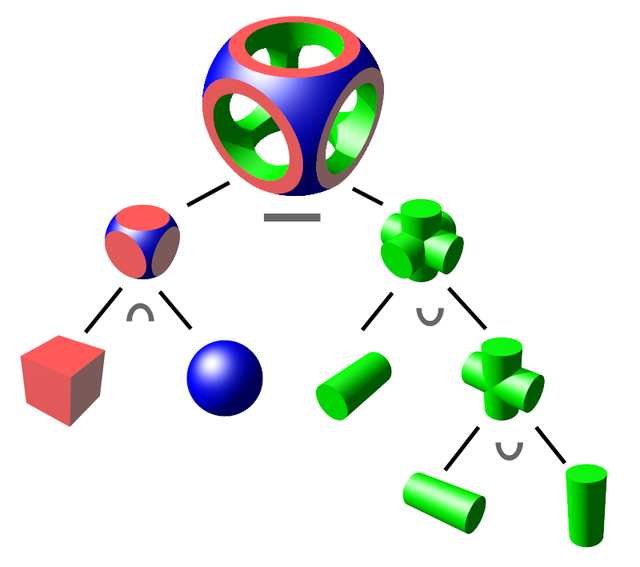
\includegraphics[width=0.4\textwidth]{images/Hardware_openscad_example.png}
        \caption{Example of a complex shape made from simple primitive objects and boolean operators.}\label{fig:hardware_openscad_example}
\end{figure} 

OpenSCAD also counts with some 2D primitives for creating objects through 2D shape extrusion, such as squares, circles and polygons, defined point by point. It also can import CAD files in DXF format for extruding them, or export 2D shapes in DXF format to use them in other CAD programs. The 2D shapes can also be combined using boolean operators, and the extruded to form 3D objects, either with a linear extrusion or with a rotate extrusion, that creates solids of revolution.\\

\begin{figure}[h]
		\centering
        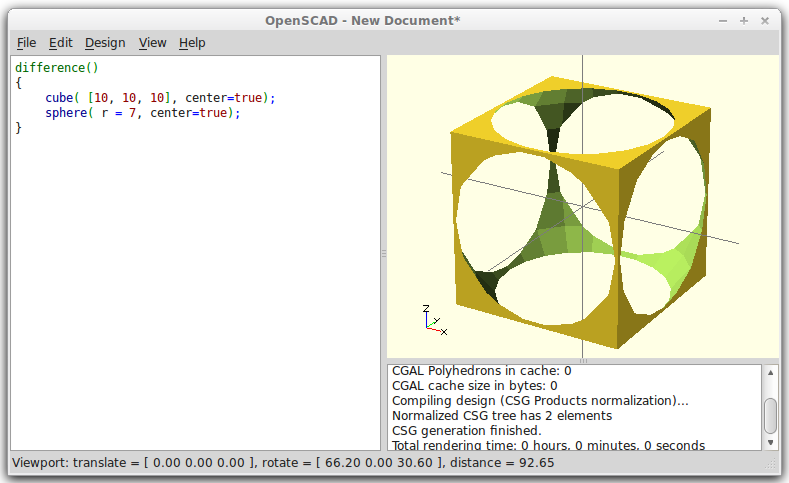
\includegraphics[width=0.7\textwidth]{images/Hardware_openscad_example2.png}
        \caption{OpenSCAD screenshot with a simple object being created.}
        \label{fig:hardware_openscad_example2}
\end{figure} 


%%%%%%%%%%%%%%%%%%%%%%%%%%%%%%%%% OOML %%%%%%%%%%%%%%%%%%%%%%%%%%%%%%%%%%%%%%%%%%%%%%%%%%%%%%%%%%%%%%%%%%%%
\subsubsection{Object-Oriented Mechanics Library (OOML)}
\label{hardware_software_ooml}

The Object-Oriented Mechanics Library \cite{ooml:website, Valero-Gomez2012} is an open source C++ library to model 3D objects using C++, in a similar way as the objects are described with OpenSCAD. It was developed by Juan Gonzalez-Gomez and Alberto Valero-Gomez as a way to extend the capabilities of OpenSCAD with the features available in more advanced programming languages such as objects, inheritance or operator overloading, as well as the existing libraries for those languages to, for example, perform mathematical operations.\\

OOML counts with the same primitive 3D objects of OpenSCAD (cube, cylinder and sphere), plus some additional components such as toroids, prisms, rounded tablets, rounded cubes, rounded cylinders or text strings. It also offers the same 2D primitives, and boolean operations, that can be performed with the classic C++ operators: ``$+$'' for union, ``$-$'' for difference and ``$*$'' for intersection.\\

Apart from the basic primitive objects, OOML has also a part library with 
more complex, basic objects with a mechanical meaning, that can be combined to form even more complex mechanisms, such as robots. These objects are parametric, so they can be reused across designs, and derivative objects can be made based on these ones by using C++ inheritance. This library contains wheels, battery holders, batteries, servos, sensors, etc.\\

\begin{figure}[h]
		\centering
        \begin{subfigure}[b]{0.49\textwidth}
                \centering
                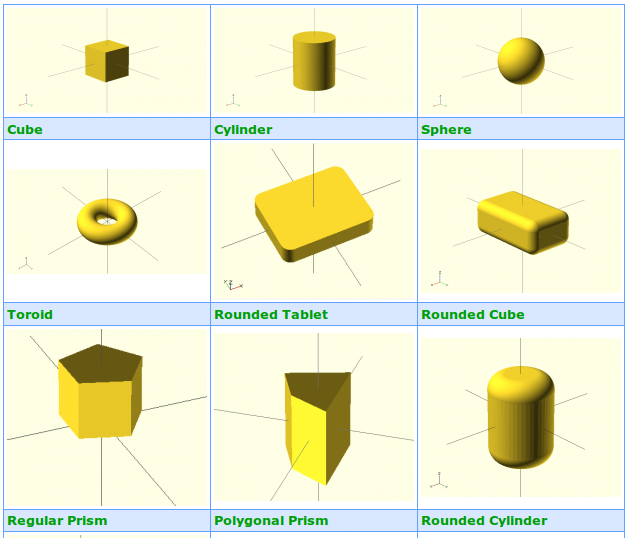
\includegraphics[width=\textwidth]{images/Hardware_ooml_primitives.png}
                \caption{Primitive objects}
                \label{fig:hardware_ooml_primitives}
        \end{subfigure}
        ~
        \begin{subfigure}[b]{0.45\textwidth}
                \centering
                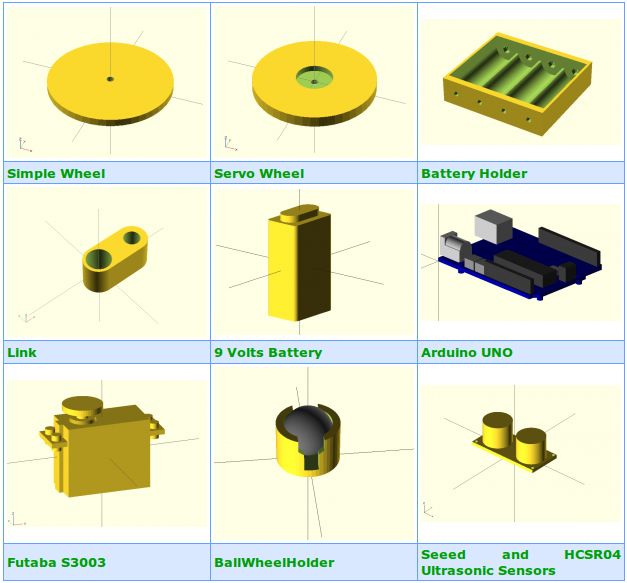
\includegraphics[width=\textwidth]{images/Hardware_ooml_parts.png}
                \caption{Parts}
                \label{fig:hardware_ooml_parts}
        \end{subfigure}
        \caption{OOML's primitive objects and parts}
        \label{fig:hardware_ooml_example}
\end{figure}

From the compoment object, OOML automatically generates OpenSCAD code that can be used to render and compile the object in the OpenSCAD development environment. For the code generation OOML has a class, called \emph{Writer}, that is in charge of converting the description of a 3D object into OpenSCAD code.\\

%%%%%%%%%%%%%%%%%%% Previous work %%%%%%%%%%%%%%%%%%%%%%%%%%%%%%%%%%%%%%%%%%%%
\subsection{Previous work}
\label{hardware_previouswork}

On the state of the art, we introduced several platforms for developing modular robotics. For developing our module we reviewed all of them, and we decided not to reinvent the wheel starting a new design from scratch, so we selected an existing open platform, the Y1 module and its derivatives.

\subsubsection{Y1 module}
\label{hardware_y1}

The Y1 module \cite{gonzalez-gomez_website:y1} was developed by Juan Gonzalez-Gomez for his PhD thesis, as a open and cheap platform to study locomotion of modular robots. The Y1 modules are based on the G1 modules designed by Mark Yim \cite{Yim2000} for the PolyBot robot (the letter `Y' in Y1 stands for ``Yim'' in his honor).\\

Y1 modules are composed of a cheap hobby servo and a two-part housing made from several pieces of laset cut PVC glued together. These modules can be connected in a linear configuration, either pitch-pitch or pitch-yaw, allowing the resulting robots to move in a plane. As the main objective of Gonzalez-Gomez's thesis was to study only the locomotion of modular robots, the resulting design is very simple, and the connections between modules are achieved with screws. As the module does not have any active connector, reconfiguration has to be done by hand. For the same reasons, the control electronics and the power source were supplied off-board.\\

The main reasons for basing the design of our module mainly on the Y1 module are the following:

\begin{itemize}
	\item \textbf{Open Source Hardware.} The Y1 module is open source hardware, which means that the plans, the files for manufacturing and the assembly instructions are publicly available online for anyone to access them, study them, and improve them, offering a good starting point for a new design. 
	
	\item \textbf{Low-cost.} Even though the robots made from Y1 modules can only work tethered and are no self-reconfigurable, their extremely low cost compared with the previously mentioned platforms and the public availability of its sources make the Y1 modules a perfect choice for studying locomotion gaits for modular robots in labs with a reduced budget, or for introducing undergraduate students, or even kids \cite{gonzalez-gomez_website:taller_2010}, to modular robotics.
	
	\item \textbf{Availability of materials and easiness of assembly.} The Y1 modules are made of PVC plastic, which is very easy to find in any hardware store. The parts that compose the module housing can be cut from that plastic either by hand or using a laset cutting machine, and later glued together to form the housing. This housing is assembled together using screws, making the whole assembly process very easy to perform.\\
	
\end{itemize}

\begin{figure}[h]
		\centering
        \begin{subfigure}[b]{0.3\textwidth}
                \centering
                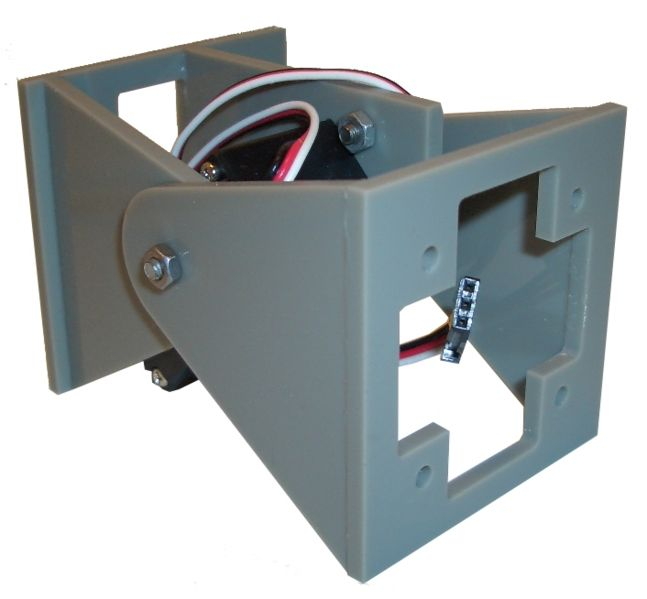
\includegraphics[width=\textwidth]{images/Y1_01.jpg}
                \caption{Y1}
                \label{fig:hardware_y1_mod}
        \end{subfigure}
        ~
        \begin{subfigure}[b]{0.3\textwidth}
                \centering
                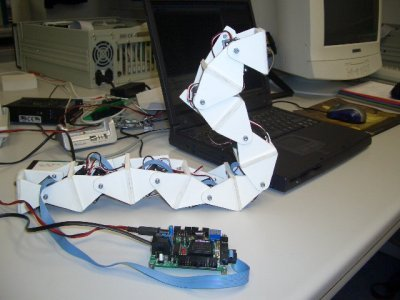
\includegraphics[width=\textwidth]{images/State_art_Y1_cube.jpeg}
                \caption{Cube Revolutions (Y1 snake)}
                \label{fig:hardware_y1_cube}
        \end{subfigure}
        \caption{Module Y1} \label{fig:hardware_y1}
\end{figure}

\newpage
\subsubsection{Y1 module derivatives: MY1 and REPY1}
\label{hardware_repy1}

Based on the Y1 design, Gonzalez-Gomez developed other modules: the MY1 and the REPY-1. The MY1\cite{gonzalez-gomez_website:my1} is a metal version of the Y1 module, manufactured from 2mm thick aluminium with a similar shape to the Y1, and compatible with it. A battery holder and a control board were designed for this module, therefore allowing untethered operation of the robots constructed with this module.\\

The advantages of the MY1 module are a stronger frame, and the incorporation of the control board and power in the robot structure, requiring only either a serial connection with the computer to be controlled, or having the movements loaded on the controller board. This advantages, however, imply a higher cost and a more complicated manufacturing process, increasing the price of the modules.\\

The REPY-1\cite{gonzalez-gomez_website:repy1} module (REPlicable Y1) is a version of the Y1 designed to be printed in a low cost 3D printer, like a RepRap\cite{jones_reprap_2011}. This simplifies the assembly of the module, as it reduces the number of parts to 2, which can be produced at a low price. If printed on a RepRap 3D printer such as a Prusa Medel 3 model, that costs around 300\euro, the filament material to print both module halves costs no more than 1-2\euro.\\

Apart from the reduced cost and even further simplification of the assembly process, the REPY-1 module has other advantages with respect to the Y1 module. Since the 3D printing process does not imply high fixed manufacturing costs (such as material handling costs, set-up costs, mainteinance costs, etc) there is no need to produce a large batch of modules. Instead, modules can be printed one by one as they are needed. This also allows a faster and cheaper prototyping and improvement process, as modules can be produced, assembled and tested in a short period of time at a low price. Improvements can be done to them, and a new batch of the next iteration of prototypes can be manufactured in a short time and at a low cost, achieving a evolution in the design that previously was only possible to be done in software products.\\

\begin{figure}[h]
		\centering
        \begin{subfigure}[b]{0.3\textwidth}
                \centering
                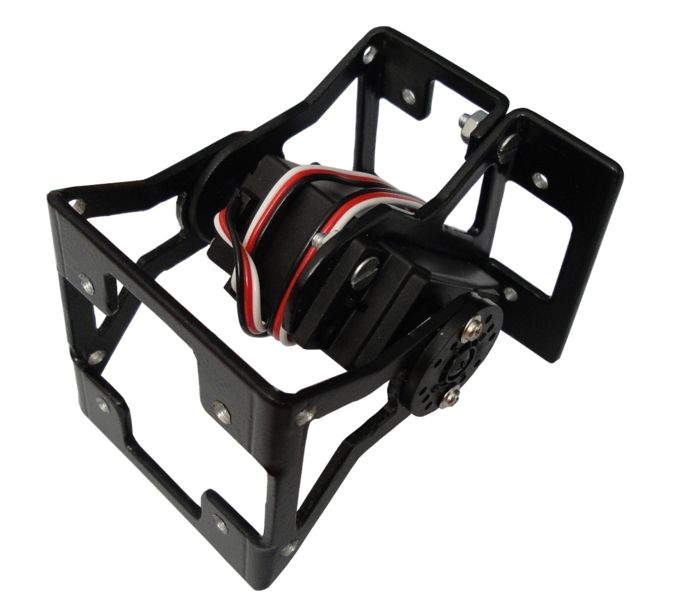
\includegraphics[width=\textwidth]{images/Y1_MY1_01.jpg}
                \caption{MY1}
                \label{fig:hardware_my1}
        \end{subfigure}
        ~
        \begin{subfigure}[b]{0.3\textwidth}
                \centering
                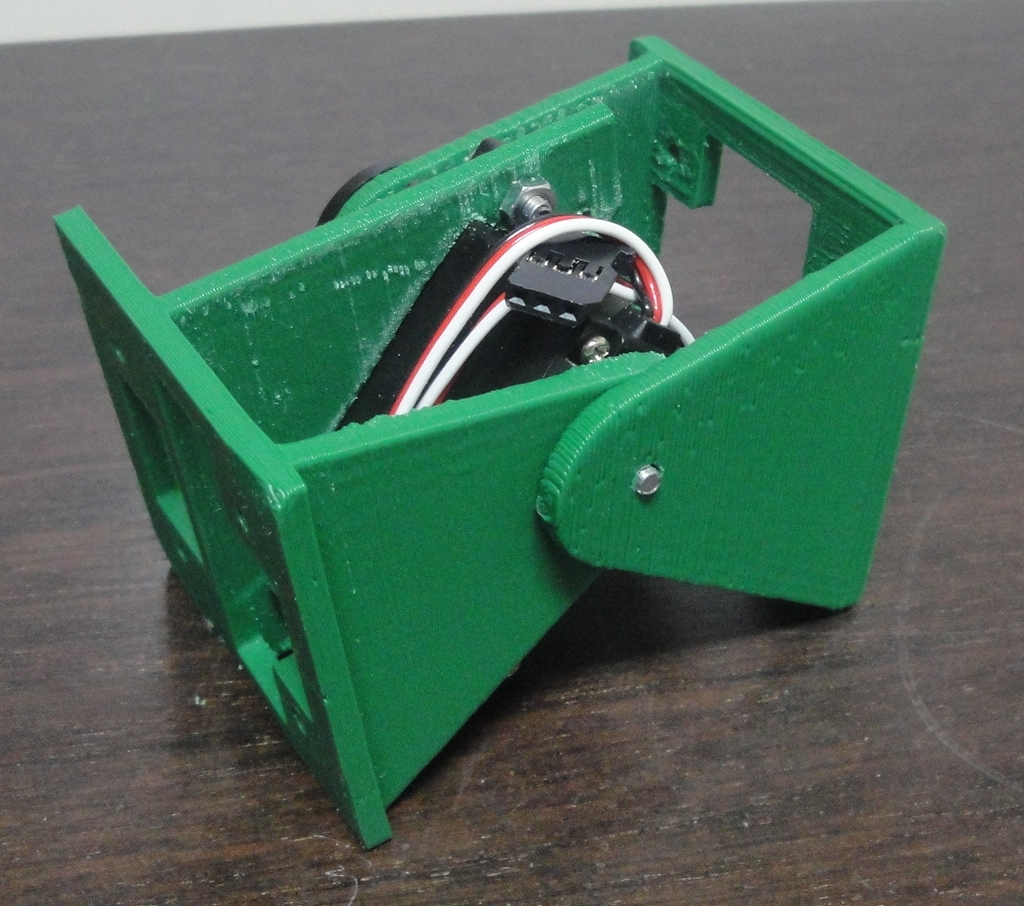
\includegraphics[width=\textwidth]{images/Y1_REPY1_01.jpg}
                \caption{REPY-1}
                \label{fig:hardware_repy1}
        \end{subfigure}
        \caption{Module Y1 derivatives: MY1 and REPY-1} \label{fig:hardware_y1_derivatives}
\end{figure}

The MY1 and REPY-1 modules are also open source, and the files to manufacture them are available in Gonzalez-Gomez's website, with assembly and usage instructions. Having the files publicly available allowed us to download them and print a small batch of 4 REPY-1 modules in order to test them and evaluate their virtues and flaws, in order to improve the design later. We will discuss those improvements made to the original Y1 design on the next section about our design, the REPY-2 module.\\

%%%%%%%%%%%%%%%%%%% REPY-2.x %%%%%%%%%%%%%%%%%%%%%%%%%%%%%%%%%%%%%%%%%%%%
\newpage
\subsection{REPY-2}
\label{hardware_repy-2.x}

Several REPY-1 modules were printed and analyzed on different configurations in order to find if they could be used in this project. After testing them, we realized that the design was a good starting point, but it needed to be improved in order to be used for this thesis.\\

Based on our analysis and tests of the printed version of the Y1 module, the REPY-1 module, we observed the following problems in the module design:

\begin{itemize}
	\item The design was difficult to print correctly and it was very fragile. The part that holds the hobby servo was connected to the rest of the body of the module by a small section that broke while it was being printed, and one of the ears of the module was too thin, so it usually broke when assembling both halves together. 
	
	\item The REPY-1 was designed on OpenSCAD, but it imported the DXF files of the laser-cut Y1 module, extruded them and placed them together, so the module was not parametric. This means that this design only works with the Futaba 3003s hobby servo and the Skycube/Skymega board. This design is therefore not easy to modify or adapt to other hardware different from the original one.
	
	\item The module REPY-1, as well as the module Y1 are not symmetric, since they have the hobby servo placed at an angle of approximately 45º with respect to the base. This results in a more compact module, but allows locomotion of robots only when placed over one of their sides, the opposite one has a straight spine that contains the servo and makes the gait unstable.
	  
	\item Only 2 connectors are present on the Y1 modules and their derivatives, on the front and the back of the module, so the possible configurations that can be assembled with them are restricted to chain-type, 1D configurations. This makes them only suitable for testing locomotion in apodal robots, such as snake robots.
	  
\end{itemize}

Other improvements, such as an active connector to enable self-reconfiguration, or a control board and power management system integrated on each of the modules were also desirable, but discarded due to the temporal and economic constraints of this project.

\subsubsection{First version: REPY-2.0}
We started the design of the module in OpenSCAD, but soon we moved to OOML, since the C++ language allowed us to perform more powerful operations with a clearer syntax. Designing the module with the OOML library instead of directly on OpenSCAD also allowed us to organize the code better, helped by the use of C++ classes.\\

This first version, called REPY-2.0, solved most of the issues found on the original REPY-1 module. The module was designed not just parametric, but object-oriented. This means that a \emph{BasicServo} class and a \emph{BasicPCB} class exist, containing all the dimensions that define the hobby servo and the control board. Instances of these classes are passed to the constructor of the \emph{REPY\_module} class, that uses the stored dimensions to generate automatically a module suitable for being used with that servo and control board. If one wants to build the module with a different model of hobby servo, or with a different control board, he just has to define new servos or PCBs, by inheriting the basic interface from the \emph{BasicServo} and \emph{BasicPCB} classes. If the \emph{REPY\_module} constructor is called with these new servos or PCBs, it will automatically generate a module to be used with them.\\

The module was made symmetrical by placing the hobby servo at a 90º angle with respect to the base of the module, allowing a smooth movement of the module on either of its opposing sides, solving the instablity problem of the Y1 module when placed over the straight side of the module body.\\

The overall design was reinforced so that it was easier to print and stronger, being less likely to break it when assembling the module. The thickness of the walls was increased as thin walls were a frequent cause of failure when printing the REPY-1 module and they broke easily. This thicker walls also allowed the horn of the servo to be embedded in the module upper part,  eliminating the need of using screws to fix the servo horn to the module.\\

This module version was printed for the Futaba 3003s servo with a Skymega board and, in order to test that this design could also generate modules to use with other servos and boards, we also print a smaller version of the module to assemble with the smaller Towerpro SG90 servo, and a small, custom board. Figure \ref{fig:hardware_repy2_big_and_small} shows the two kinds of REPY-2.0 modules printed to test the design. It is important that both modules were generated from the same code, only changing the servo and board objects passed to the module constructor.\\

\begin{figure}[H]
		\centering
        \begin{subfigure}[b]{0.45\textwidth}
                \centering
                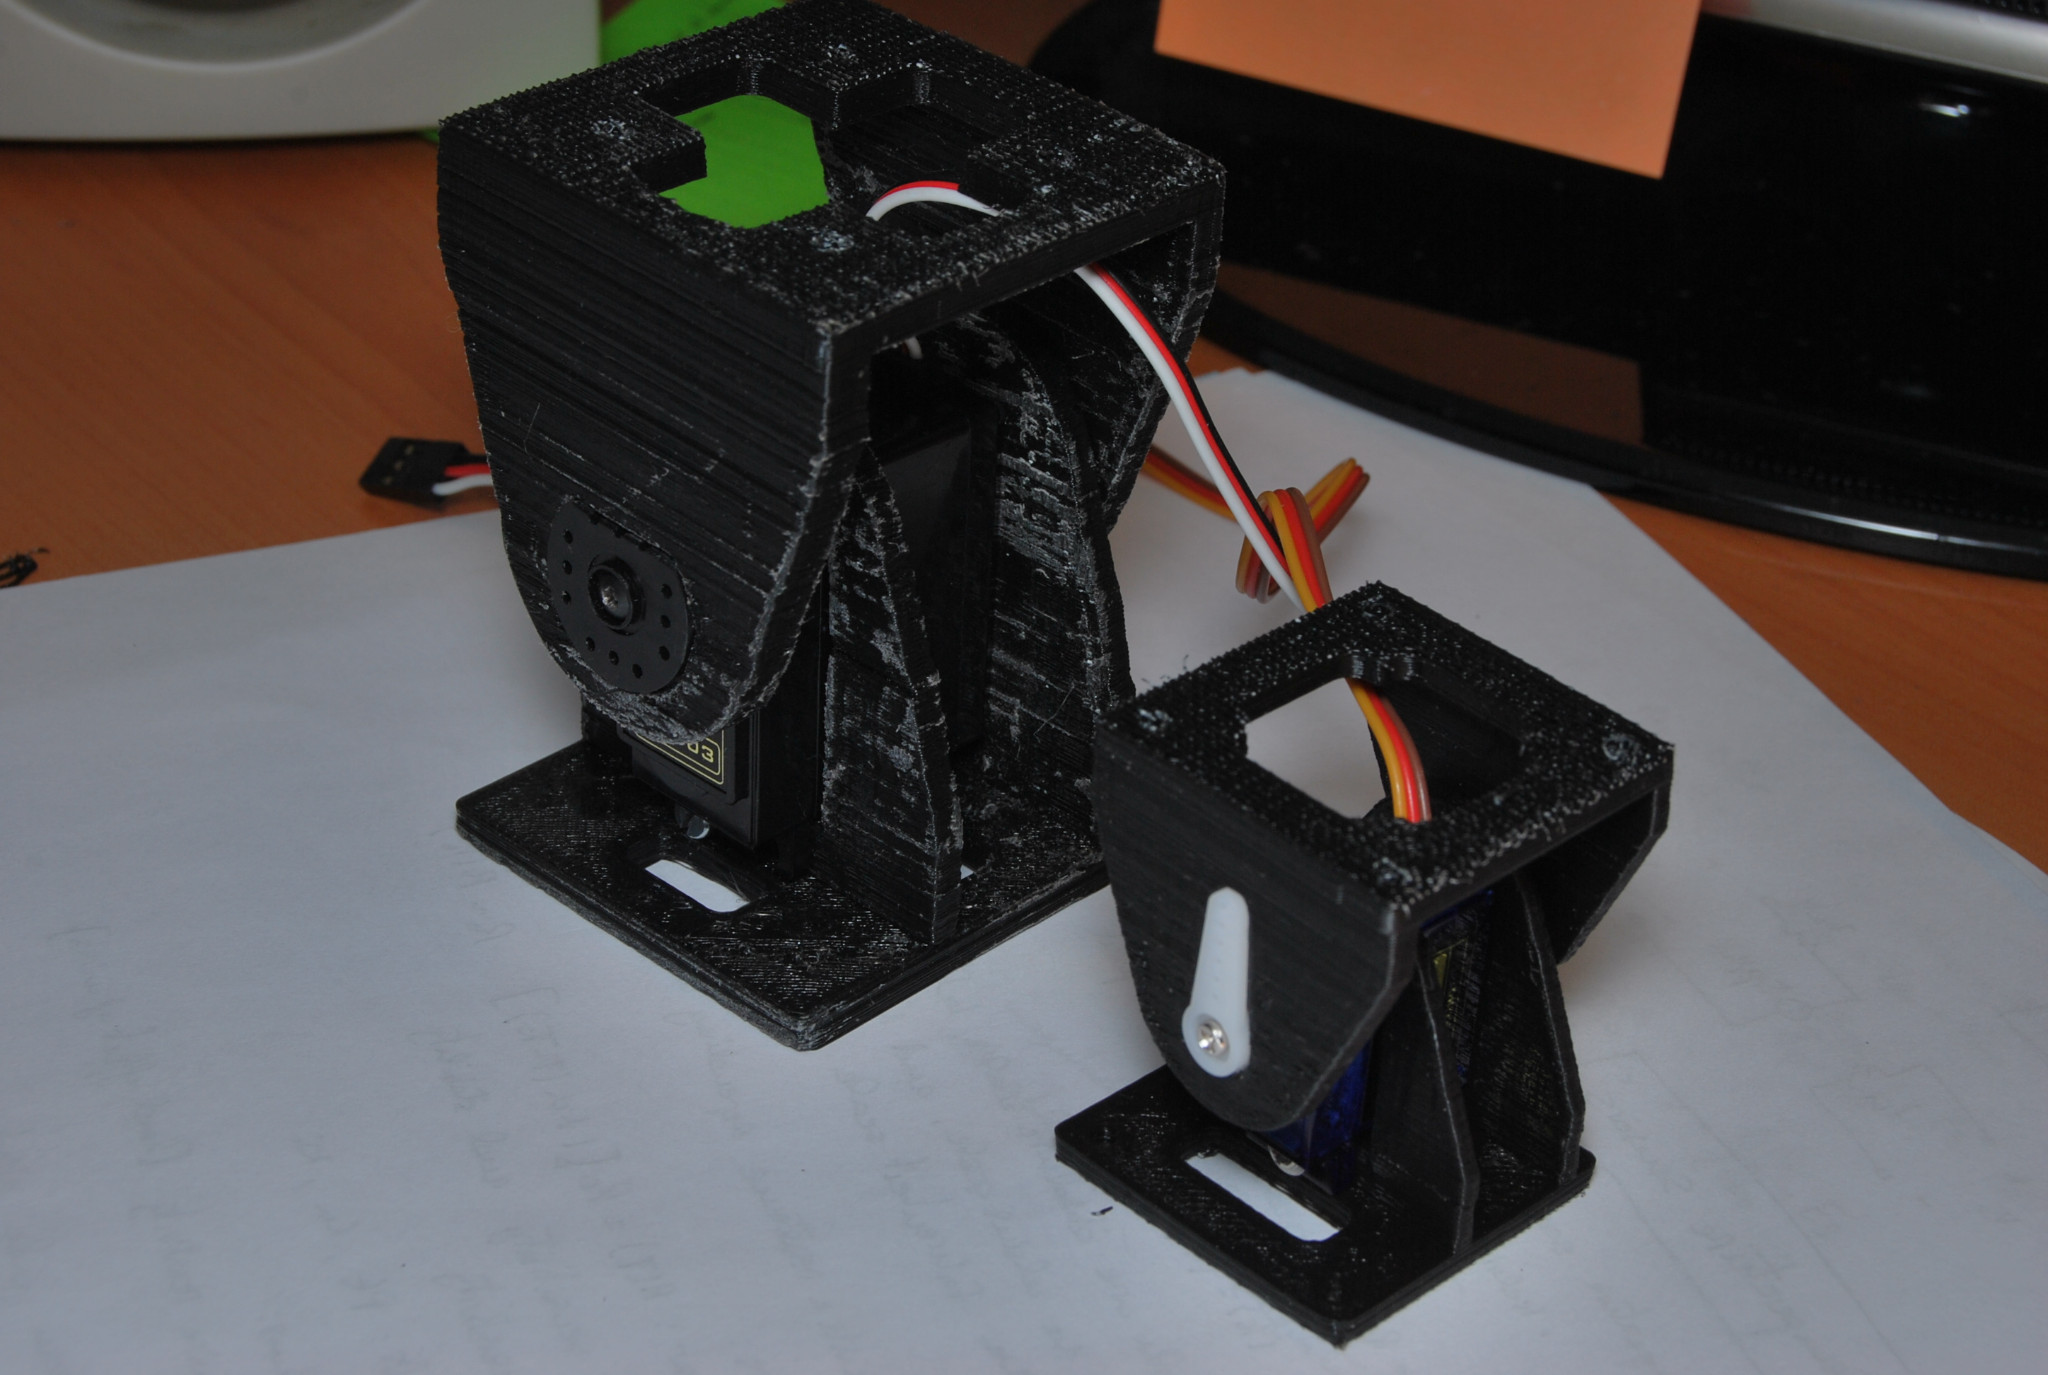
\includegraphics[width=\textwidth]{images/Hardware_repy2_big_and_small_01.jpg}
                \label{fig:hardware_repy2_big_and_small_01}
        \end{subfigure}
        ~
        \begin{subfigure}[b]{0.45\textwidth}
                \centering
                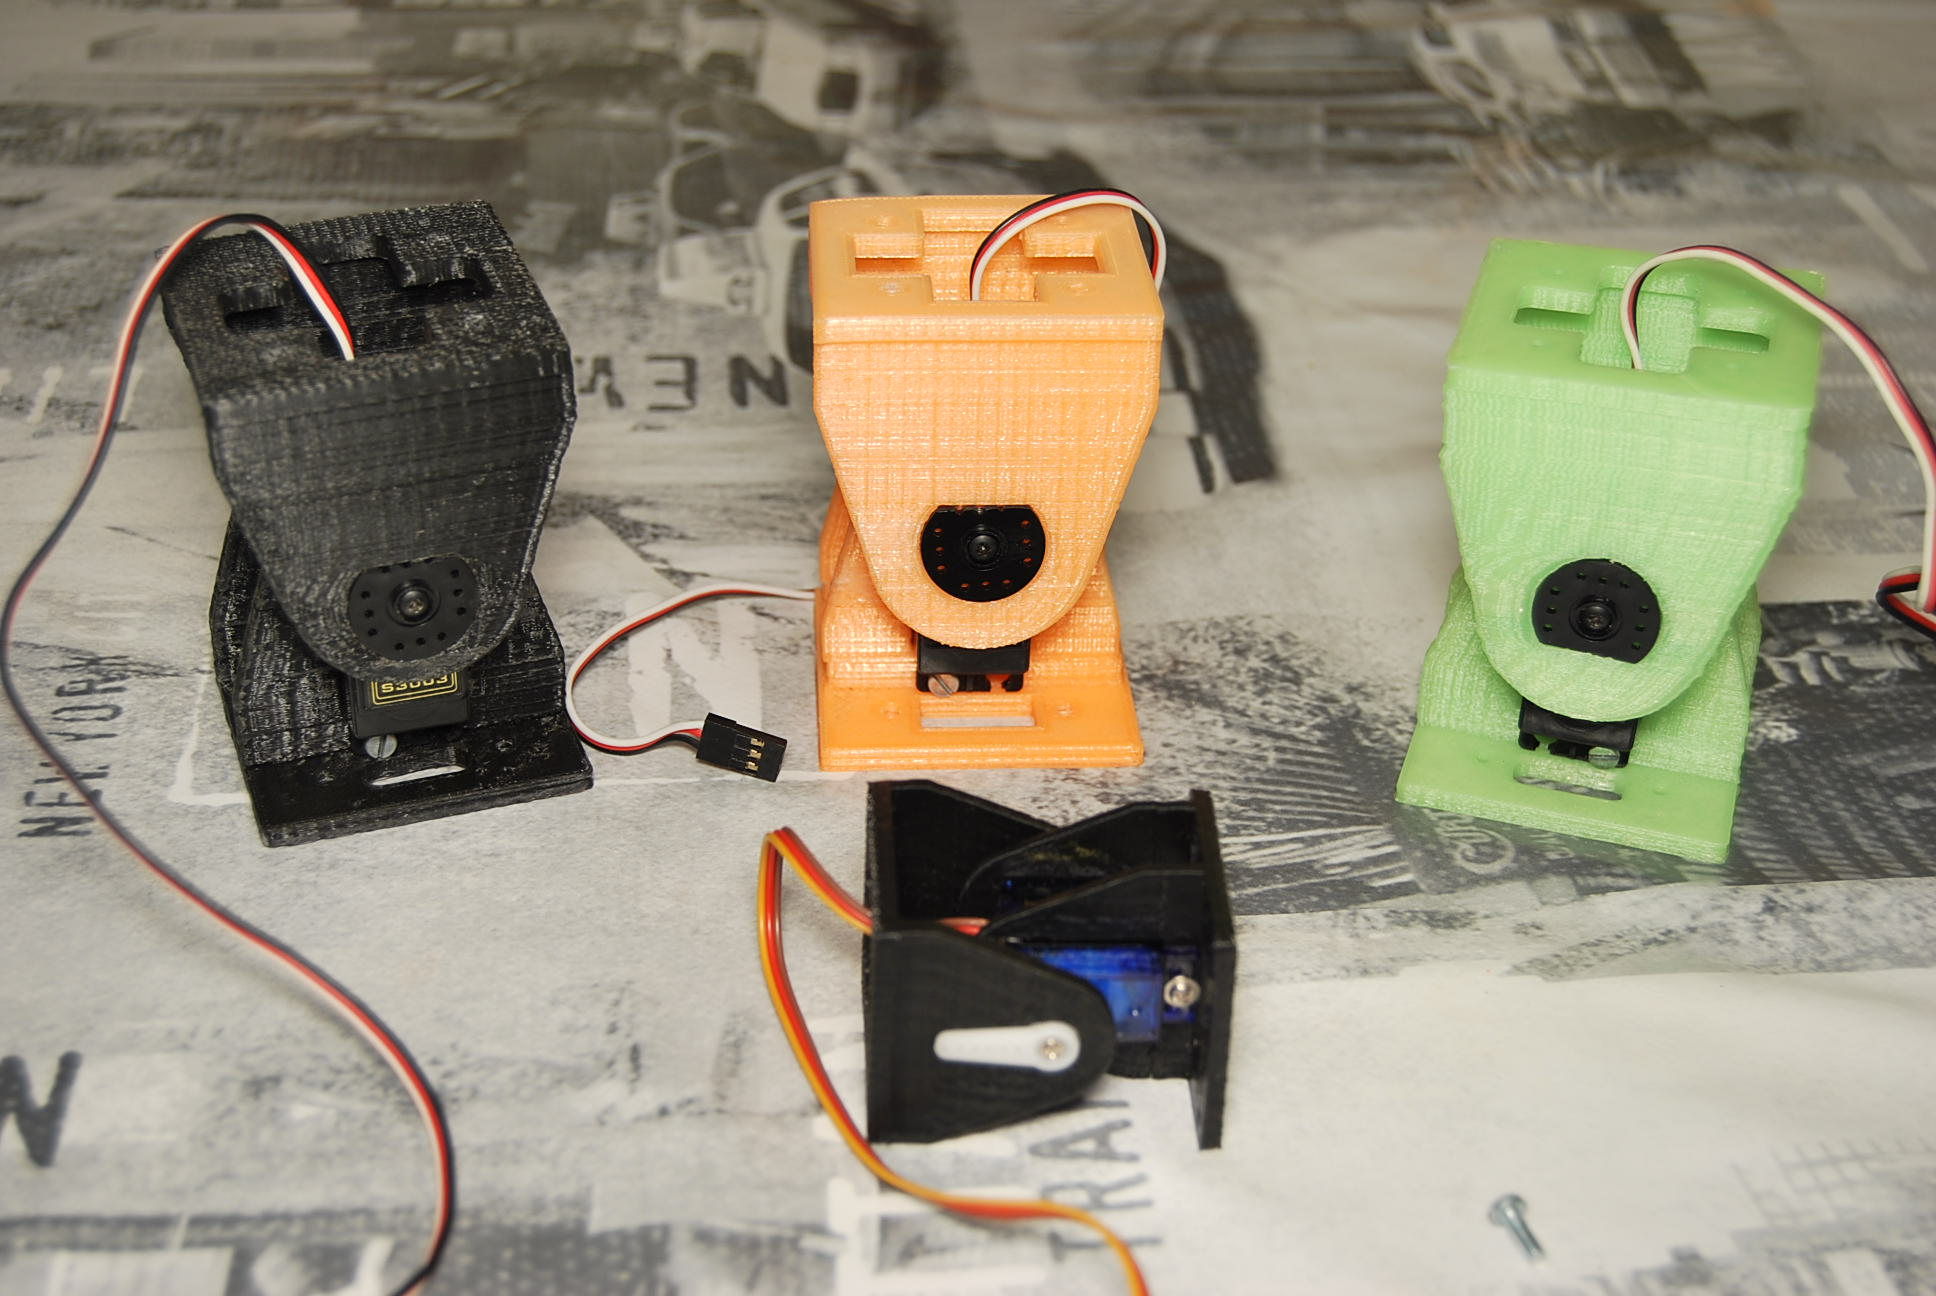
\includegraphics[width=\textwidth]{images/Hardware_repy2_big_and_small_02.jpg}
                \label{fig:hardware_repy2_big_and_small_02}
        \end{subfigure}
        \caption{Two different REPY-2.0 modules for different servos generated from the same code. } \label{fig:hardware_repy2_big_and_small}
\end{figure}


\subsubsection{Second version: REPY-2.1}

A second version of the REPY-2 modules was developed shortly after testing and validating the first version. This version is mostly equal to the first version, but the tolerances for the different fittings are better adjusted. The last of the required improvements, two side connectors for enabling 2D configurations were also added in this version. These connectors are just 4 holes in the same disposition than the holes in the front and back of the module, that allow the connection with other modules with screws, as the front and back connectors did.\\

Since both versions are compatible (in both connector and dimensions), and the main difference is the presence of two extra side connectors, both versions were used to assemble the modular robots to test the locomotion gaits, using the second version ones for the places were a 2D connection between modules were used. This way we could use the first version modules already printed to reduce the number of required modules of the second version.\\

\begin{figure}[H]
		\centering
        \begin{subfigure}[b]{0.4\textwidth}
                \centering
                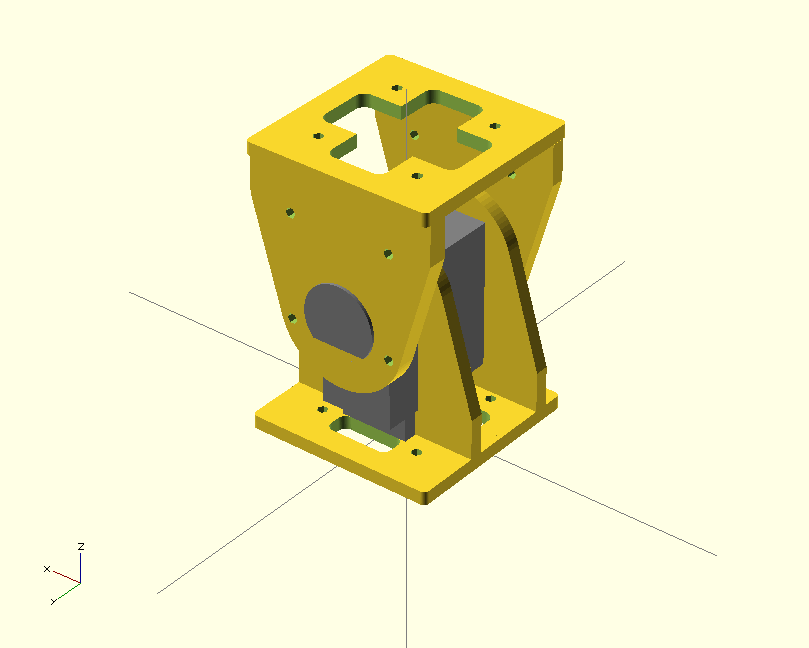
\includegraphics[width=\textwidth]{images/Gait_osc_center_90.png}
                \caption{OpenSCAD render of REPY-2.1 module.}
                \label{fig:hardware_repy2_1_render}
        \end{subfigure}
        ~
        \begin{subfigure}[b]{0.32\textwidth}
                \centering
                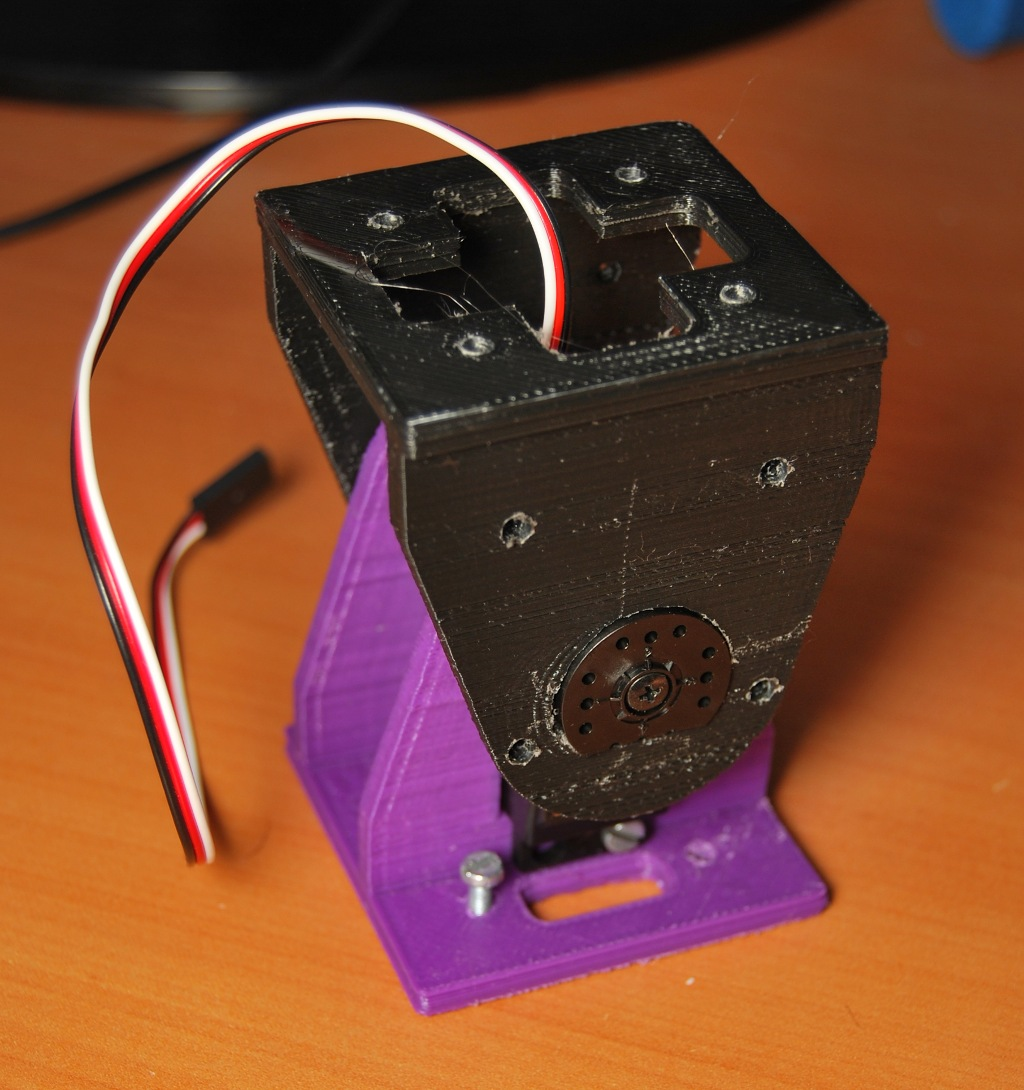
\includegraphics[width=\textwidth]{images/Hardware_REPY_2_1_real.jpg}
                \caption{Printed REPY-2.1 module.}
                \label{fig:hardware_repy2_1_real}
        \end{subfigure}
        \caption{REPY-2.1 modules.} \label{fig:hardware_repy2_1}
\end{figure}


%%%%%%%%%%%%%%%%%%%%%%%%%% Code Structure %%%%%%%%%%%%%%%%%%%%%%%%%%%%%%%%%%%%%%%%%%%%%%%%%%%%%%%%%%%%%%%%%%%%
\subsection{REPY-2.1 OOML code structure}
\label{hardware_ooml_structure}

\begin{figure}[h]
		\centering
        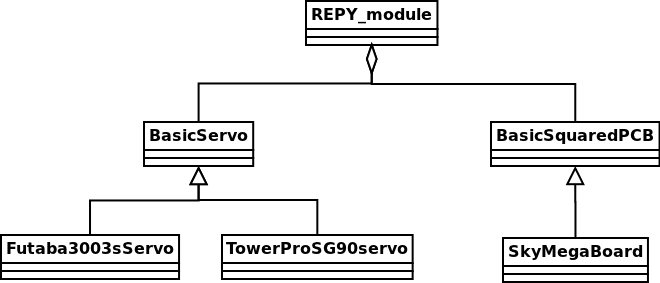
\includegraphics[width=0.7\textwidth]{images/REPY2_class_diagram_main.png}
        \caption{Main class diagram}
        \label{fig:hardware_class_diagram_main}
\end{figure} 


The OOML code for describing the REPY-2 module has a main class, called \emph{REPY\_module}, that defines the geometry of the whole module (both upper and lower parts). This class takes as arguments a servo object that follows the \emph{BasicServo} abstract interface and a PCB object that implements the \emph{BasicSquaredPCB} abstract interface. From this objects the \emph{REPY\_module} extracts the key dimensions and uses them to calculate its own dimensions and geometry automatically. The main class diagram for the module OOML code is shown in figure \ref{fig:hardware_class_diagram_main}.\\

This section will explain the main classes used to model the REPY-2 module with the OOML. More detailed information about the code, useful for developers interested in understanding the code and contribute to the project with new servos, boards or improvements can be found documented online on \url{http://www.dsquaredrobotics.com/wiki/doku.php?id=en:repy-2.0} .\\

The code of the REPY-2 module is open source, and can be found in the following repository: \url{https://github.com/David-Estevez/REPY-2.0} .

\subsubsection{Class REPY\_module}

\begin{figure}[h]
		\centering
        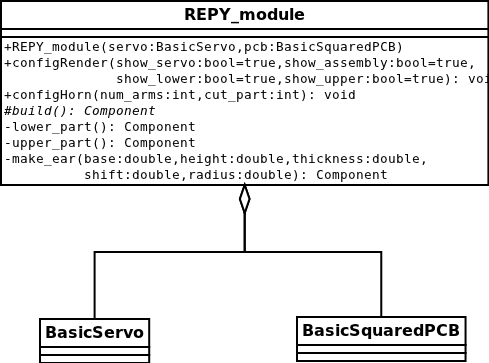
\includegraphics[width=0.5\textwidth]{images/REPY2_class_diagram_REPY_module.png}
        \caption{Class diagram for REPY\_module}
        \label{fig:hardware_class_diagram_REPY_module}
\end{figure} 

The class \emph{REPY\_module} generates the geometry of the module. It extracts the required dimensions from a \emph{BasicServo} and a \emph{BasicSquaredPCB} and calculates its own dimensions from them.\\

With the function \emph{configRender()} the user can specify if the OpenSCAD code generated from this OOML component will represent the upper part of the module, the lower part of the module or both, apart from other options as if those parts will be shown in an assembly view or in a position ready to be printed as well as if the servo will be shown or no. It is also possible to select the servo horn to be used between the ones available for each servo with the function \emph{configHorn}.\\

The upper and lower part are defined in different private functions, \emph{lower\_part()} and \emph{upper\_part()}, that are called by the function \emph{build()}, which generates the whole model depending on the configuration parameters selected. As both parts of the module use a similar shape for their sides, a function \emph{make\_ear()} is defined to create them easily.\\


\subsubsection{Class BasicSquaredPCB}
\begin{figure}[h]
		\centering
        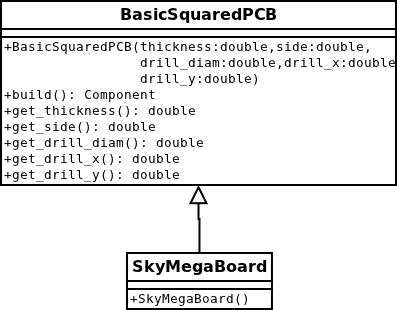
\includegraphics[width=0.5\textwidth]{images/REPY2_class_diagram_BasicSquaredPCB.png}
        \caption{Class diagram for BasicSquaredPCB}
        \label{fig:hardware_class_diagram_BasicSquaredPCB}
\end{figure} 

The class \emph{BasicSquaredPCB} represents a simple squared PCB with four holes for placing screws to attach it to the module. It is defined by the length of the side, the thickness of the PCB, and the location and radius of the drills for the screws.\\

The SkyMega board dimensions are included in the \emph{SkyMegaBoard}, that is used to create the standard size module. For the small module, a custom board was defined using the constructor of the \emph{BasicSquaredPCB}  class.\\


\subsubsection{Class BasicServo}

Hobby servos can be created using as a base the \emph{BasicServo} class. The main dimensions of the servo are included in this class, and can be accessed with the getter functions. This way the \emph{REPY\_module} class can extract the main dimensions of the servo to calculate its own dimensions. The class diagram of figure \ref{fig:hardware_class_diagram_BasicServo} shows the getter functions available to request the servo dimensions.\\

\begin{figure}[h]
		\centering
        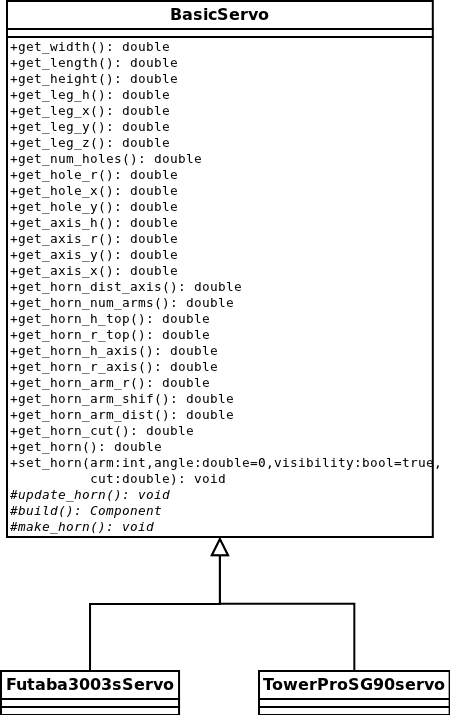
\includegraphics[width=0.5\textwidth]{images/REPY2_class_diagram_BasicServo.png}
        \caption{Class diagram for BasicServo}
        \label{fig:hardware_class_diagram_BasicServo}
\end{figure} 

Different horns can be defined for a servo, and selected with the \emph{set\_horn()} function. This horn is later created on the \emph{build()} method using the \emph{make\_horn()} with the rest of the module.\\

Two different servos were defined, the \emph{Futaba3003sServo} for the standard size module and the \emph{TowerProSG90Servo} for the smaller one. These classes contain the dimensions of the Futaba 3003s servo and the Tower Pro SG90 servo respectively, as well as some horns with different number of arms for each one.\\

\newpage
\subsection{Building the REPY-2.1 module}
\label{hardware_assembly}
In this section we will explain how to build and assemble a REPY-2.1 module. The files required for manufacturing the two parts that compose the module can be downloaded from the internet, as we are making them publicly available with an open source license.

\subsubsection{Generating the 3D files}

The first step to build the REPY-2 modules is to obtain the STL files in order to print the parts of the module. These files can be downloaded from the module repository: \url{https://github.com/David-Estevez/REPY-2.0} , or compiled from the source code.\\

The requirements for obtaining the files from the sources are the following:
\begin{itemize}
	\item \textbf{CMake.} CMake is used to generate the makefiles used to compile the project C++ code. CMake can be downloaded from \url{http://www.cmake.org/cmake/resources/software.html}. More detailed instructions can be found on section \ref{software_install_cmake}.
	
	\item \textbf{OOML.} The Object Oriented Mechanics Library allow us to generate OpenSCAD code from the C++ code, and can be downloaded from \url{http://iearobotics.com/oomlwiki/doku.php?id=start} . The website counts with very detailed instructions for installing OOML.
	
	\item \textbf{OpenSCAD.} The OOML only generates OpenSCAD code. For obtaining the STL files, OpenSCAD is required. It can be downloaded from its website: \url{http://www.openscad.org/} .\\
\end{itemize}

Once the dependencies are installed, the code has to be built. The instructions for building the code are:
\begin{enumerate}
	\item Edit the file ``CMakeLists.txt'' to include the path to the OOML include directory. For example, in the authors system this path was ``/usr/include/ooml''.

	\item Open a terminal, go to the REPY-2.0 directory and build it using cmake:
        \Bash
		\begin{lstlisting}
	$ mkdir build
	$ cd build
	$ cmake ..
	$ make 
	$ make install
		\end{lstlisting} %$	
Notice that for the installation you won't need to be superuser, as it is installed in a directory called \emph{`bin'} in the \emph{`REPY-2.0 folder'}.

	\item Execute the program \emph{REPY-2.0}, that will create the SCAD files and, optionally, the STL files for the REPY-2.0 module.
	
	\item If the STL files were not generated using the \emph{REPY-2.0} program, open the desired SCAD file with OpenSCAD  and compile it manually.
\end{enumerate}

\newpage
\subsubsection{Printing the parts}

Once the STL files have been downloaded or generated, the next step is printing them on the 3D printer. The concrete steps that are to be followed to print depend on the 3D printer that is going to be used and the software to control it. These low-cost 3D printers used create the object by depositing plastic layer by layer until the object is complete. The plastic used is tipically ABS (Acrylonitrile butadiene styrene) or PLA (Polylactic Acid)\\

The steps required to print the files involve usually to generate the GCODEs (codes that are control the CNC machine, specifying the velocity and position of its tool, in this case, the plastic extruder required to follow the required path, as well as the amount of plastic to extrude in each position) with a slicer software. The slicer software calculates those toolpaths by slicing the 3D models in several planes, and calculating the trajectories required in each layer to form the 3D object.\\

For the module to be assembled two parts need to be printed: the lower part and the upper part. As hobby servos usually come with more than one horns with different geometries available, there are more than one upper parts in the repository, each one to be used with a different type of horn. Only one upper part is needed to build the module, that has to be selected according to the horn to be used.


\subsubsection{Assembling the module}

\noindent
Each module requires the following materials to be built:
\begin{itemize}
	\item 1x Upper part of the module (3D printed part)
	\item 1x Lower part of the module (3D printed part)
	\item 1x Futaba 3003s servo
	\item 1x M3x8mm screw
	\item 4x M3x10mm screws (minimum 2)
	\item 4x M3 nuts (minimum 2)
	\item 4x M3 washers (minimum 2)
\end{itemize}

\newpage

\begin{figure}[H]
		\centering
        \begin{subfigure}[b]{0.46\textwidth}
                \centering
                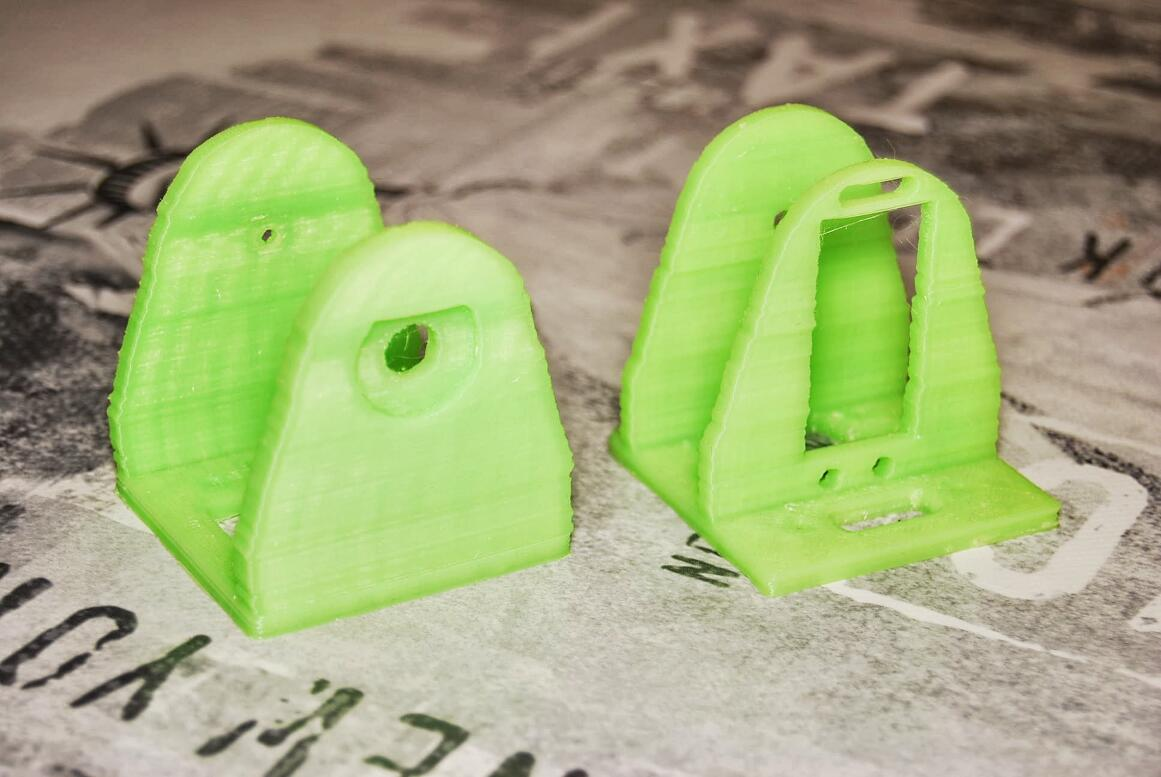
\includegraphics[width=\textwidth]{images/REPY2_assembly_01.jpg}
                \caption{Printed plastic parts needed: upper part and lower part.\\}
                \label{fig:hardware_assembly_01}
        \end{subfigure}
        ~
        \begin{subfigure}[b]{0.46\textwidth}
                \centering
                \includegraphics[width=\textwidth]{images/REPY2_assembly_02.jpg}
                \caption{Overview of tools and parts needed for assembling the module.}
                \label{fig:hardware_assembly_02}
        \end{subfigure}
        \caption{Required materials to build the REPY-2.1 module} 
        \label{fig:hardware_assembly_materials}
\end{figure}

\begin{figure}[H]
        \centering
        \begin{subfigure}[b]{0.46\textwidth}
                \centering
                \includegraphics[width=\textwidth]{images/REPY2_assembly_03.jpg}
                \caption{Insert carefully the module in the lower part in the hole prepared to hold the servo.\\}
                \label{fig:hardware_assembly_03}
        \end{subfigure}
        ~
        \begin{subfigure}[b]{0.46\textwidth}
                \centering
                \includegraphics[width=\textwidth]{images/REPY2_assembly_04.jpg}
                \caption{Check that the servo leg holes and the module corresponing holes are aligned.\\}
                \label{fig:hardware_assembly_04}
        \end{subfigure}
        ~
        \begin{subfigure}[b]{0.46\textwidth}
                \centering
                \includegraphics[width=\textwidth]{images/REPY2_assembly_05.jpg}
                \caption{Fix the servo to the module using the screws, nuts and washers for the top holes.\\}
                \label{fig:hardware_assembly_05}
        \end{subfigure}
        ~
        \begin{subfigure}[b]{0.46\textwidth}
                \centering
                \includegraphics[width=\textwidth]{images/REPY2_assembly_06.jpg}
                \caption{Fix the servo to the module using the screws, nuts and washers for the bottom holes.\\}
                \label{fig:hardware_assembly_06}
        \end{subfigure}
        \caption{Assembly of the lower part} 
        \label{fig:hardware_assembly_lower}
\end{figure}

\begin{figure}[H]
        \centering
        \begin{subfigure}[b]{0.46\textwidth}
                \centering
                \includegraphics[width=\textwidth]{images/REPY2_assembly_08.jpg}
                \caption{Materials required to assemble the upper part.\\~\\~}
                \label{fig:hardware_assembly_08}
        \end{subfigure}
        ~
        \begin{subfigure}[b]{0.46\textwidth}
                \centering
                \includegraphics[width=\textwidth]{images/REPY2_assembly_09.jpg}
                \caption{If needed, file the hole until the servo horn fits tightly on it.\\}
                \label{fig:hardware_assembly_09}
        \end{subfigure}
        ~
        \begin{subfigure}[b]{0.46\textwidth}
                \centering
                \includegraphics[width=\textwidth]{images/REPY2_assembly_10.jpg}
                \caption{With the help of some cutting pliers, cut the horn with the shape of the corresponding hole in the printed part.\\}
                \label{fig:hardware_assembly_10}
        \end{subfigure}
        ~
        \begin{subfigure}[b]{0.46\textwidth}
                \centering
                \includegraphics[width=\textwidth]{images/REPY2_assembly_11.jpg}
                \caption{After the cut, the servo horn should look like this.\\~\\~}
                \label{fig:hardware_assembly_11}
        \end{subfigure}
        ~
        \begin{subfigure}[b]{0.46\textwidth}
                \centering
                \includegraphics[width=\textwidth]{images/REPY2_assembly_12.jpg}
                \caption{Insert the horn in the corresponding hole of the upper part.\\ }
                \label{fig:hardware_assembly_12}
        \end{subfigure}
        ~
        \begin{subfigure}[b]{0.46\textwidth}
                \centering
                \includegraphics[width=\textwidth]{images/REPY2_assembly_13.jpg}
                \caption{The module should look like this seen from behind after inserting the horn.\\}
                \label{fig:hardware_assembly_13}
        \end{subfigure}
        \caption{Assembly of the servo horn} 
        \label{fig:hardware_assembly_horn}
\end{figure}

\begin{figure}[H]
        \centering
        \begin{subfigure}[b]{0.46\textwidth}
                \centering
                \includegraphics[width=\textwidth]{images/REPY2_assembly_14.jpg}
                \caption{Connect both parts carefully. The servo must be connected to the control board and set to 90º in order to ensure that the 90º position of the servo corresponds to the 90º position of the servo.\\}
                \label{fig:hardware_assembly_14}
        \end{subfigure}
        ~
        \begin{subfigure}[b]{0.46\textwidth}
                \centering
                \includegraphics[width=\textwidth]{images/REPY2_assembly_15.jpg}
                \caption{Insert the screw for the fake axis.\\~\\~\\~\\~}
                \label{fig:hardware_assembly_15}
        \end{subfigure}
        ~
        \begin{subfigure}[b]{0.46\textwidth}
                \centering
                \includegraphics[width=\textwidth]{images/REPY2_assembly_16.jpg}
                \caption{The screw of the fake axis should not protude from the servo body.\\}
                \label{fig:hardware_assembly_16}
        \end{subfigure}
        ~
        \begin{subfigure}[b]{0.46\textwidth}
                \centering
                \includegraphics[width=\textwidth]{images/REPY2_assembly_17.jpg}
                \caption{The REPY-2 module is ready to be used!\\~\\~}
                \label{fig:hardware_assembly_17}
        \end{subfigure}
        \caption{Putting together the module} 
        \label{fig:hardware_assembly_module}
\end{figure}

\newpage 

%%%%%%%%%%%%%%%%%%%%%% ELECTRONICS %%%%%%%%%%%%%%%%%%%%%%%%%%%%%%%%%%%%%%%%%%%%
\section{Electronic control board}
\label{hardware_electronics}

For the control of the robot, a controller board was designed. For this we followed the same approach that with the module, using a previous, open source design as a reference for our board, improving and fixing all the flaws we observed on the original board.\\

This section explains the software and platforms used for the design of the board software and firmware. Then, it describes the previous existent boards and the discovered weaknesses of the design. Finally, our board design is presented.


%%%%%%%%%%%%%%%%%%% Tools & software & etc %%%%%%%%%%%%%%%%%%%%%%%%%%%%%%%%%%%%%%%%%%%
\subsection{Software and platforms used}
\label{hardware_electronic_tools}

In this section we will discuss the main software tools and microcontroller platforms used. The modular robot control board, and its firmware, were developed using the Arduino platform and, for the design of our PCB, an open source program called KiCad was employed.

\subsubsection{Arduino}

Arduino \cite{arduino} is an open source electronics prototyping platform originally developed for artists, designers and hobbyists that simplifies working with microcontrolling. It is currently very extended its use in education as a first point of contact with microcontrollers, due to its simplicity.\\

The Arduino platform offers several development boards with different microcontrollers within a wide range of features, that can be selected depending on the project requirements. These boards go from the popular Arduino UNO board, that features an ATmega328, a 8-bit microcontroller with 32KB of flash and 2KB of RAM, to the latest, more advanced boards such as the Arduino DUE, that includes a 32-bit ARM processor running at 84 MHz, with 512 KB of flash and 96 KB of RAM. The schematics and CAD files for these boards are publicly available, which has promoted the appearance of several non-oficial derivative boards, Arduino-compatible, designed for concrete tasks, such as the Ardupilot, a board to control Unmanned Aerial Vehicles or the Skymega, a board for modular robotics, that will be discussed in a later section.\\

As the Arduino platform has defined a standard physical format for their development boards, some extension boards have appeared, called ``shields'', that are plugged in the development board, adding extra hardware to the Arduino boards, such as H-bridges for controlling motors or wireless transceivers for communication with other devices.\\

The principal aspects that make the Arduino easy to use are mainly two. The first one is that this platform is not limited to the hardware, but it also counts with an Integrated Development Environment (IDE) to develop the firmware to be programmed on the microcontroller and manage the board, as well as several libraries to control the microcontroller peripherals and other hardware easily. Most of these libraries have been developed by the community of Arduino users, that have published them with open source licenses for the benefit of all the Arduino community.\\

The second one is the bootloader for the Arduino boards, that allows the microcontroller to be programmed over a serial connection, and removes the necessity of a external programmer to load the firmware to the microcontroller. The process of compiling the code is also simplified by integrating the compiler toolchain into the Arduino IDE.\\

The Arduino platform has been selected over other alternatives, such as using microcontrollers from other vendors like Microchip or STMicrocontrollers because of the following reasons:

\begin{itemize}
	\item Extensive documentation and code examples can be found online due to the openness and popularity of the platform.
	
	\item The Arduino libraries reduce the development time by offering a high-level interface to the basic and advanced features of the microcontroller.
	
	\item The availability of the schematics and CAD files allows us to develop a compatible board that adapts to our requirements based on a existent and tested design, that ensures us that the hardware will work without problems, and reduces the development time.
	
	\item All this tools can be downloaded for free from the Arduino website, as opposed to other propietary IDEs, reducing the cost of the project, as no money has to be spent on development tools. 
\end{itemize}


\subsubsection{KiCad EDA Software Suite}

KiCad \cite{kicad:website} is a multiplatform, open source software suite for Electronic Design Automation (EDA). It was started by Jean-Pierre Charras, a French researcher in the field of electrical engineering, and it is composed of four main programs that perform the different functions required for the design of electronic circuits:\\

\begin{itemize}
	\item \textbf{Eeschema:} Schematic editor. This is the first step in the KiCad workflow, the creation of a schematic detailing the circuit components and connections. 
		\item \textbf{Cvpcb:} Footprint selector for components association. Once the schematic is finished, the netlist containing all the connections is generated, and the component footprints are selected from the libraries with this program.
	\item \textbf{Pcbnew:} Printed circuit board editor. After assigning the footprints to the components, the footprints and netlist are loaded in the PCB editor to make the board layout and routing. Once the PCB is designed, the GERBER files can be generated in order to manufacture the PCB.
	\item \textbf{Gerbview:} GERBER file viewer. With this program the GERBER files can be opened and inspected to check that they are correct before sending them to the manufacturer.

\end{itemize} 

For the design of the PCB in charge of the control of the robot, KiCad was used. Apart from the fact that this program is free, so no cost related to software licences was incurred, KiCad was chosen over other alternatives due to its ease of use and simplicity. Other factors that influenced the decision were that the author had previous experience with this software and the absence of limitations, such as PCB size, number of layers, etc.

%%%%%%%%%%%%%%%%%%% Previous work %%%%%%%%%%%%%%%%%%%%%%%%%%%%%%%%%%%%%%%%%%%%
\subsection{Previous work}
\label{hardware_electronics_previouswork}

For the control of the modular robots built from Y1 modules some boards already existed. Instead of designing a new board from scratch, and as the schematics of those boards were available due to them being open source, they were used as reference to design our board. As we had already worked previously with the boards in other projects, we knew the limitations of the boards to be solved in our design. The improvements added, as well as a decription of the existing boards is presented in this section.\\

\subsubsection{Skycube}
\label{hardware_skycube}

The Skycube \cite{gonzalez-gomez_website:skycube} is a board designed by Gonzalez-Gomez for controlling modular robots, featuring a PIC16F876A microcontroller running at 20MHz. It is compatible with the Y1 modules (and derivatives) and, as them, its schematics and CAD files have been released publicly with a open source license.\\

It allows the control of up to 8 hobby servos, with 4 connectors on each face to make their connection easier. Power and I2C communication connectors are also placed on both faces to allow connections on both sides of the board. The I2C bus can be used for communication between Skycube boards. The board also has a ICSP (In-Circuit Serial Programming) connector for burning the firmware with a programmer, and a connector breaking out the serial pins TX and RX, which is useful for serial communications and to upload firmware using a bootloader.\\

Even though the board counts with a connector for setting a I2C communication bus, the board is intended as a central controller for the whole modular robot, as the I2C is not a multimaster bus, and its length is limited by the capacitance of the transmission lines, as it was designed as a bus for communication between different integrated circuits inside the PCB.\\

A LED and a push button are present in the board, and can be used to interact with the program, supplying a simplistic input and output interface with the user. A expansion port is provided to the user to connect sensors or other hardware to extend the funtionality of the board.

\subsubsection{SkyMega}
\label{hardware_skymega}

The SkyMega board \cite{gonzalez-gomez_website:skymega} is a evolution of the Skycube board, designed also by Gonzalez-Gomez. The main improvement over the Skycube board is that this board substitutes the PIC microcontroller by a ATmega328 microcontroller from ATMEL, making the SkyMega Arduino-compatible, and allowing to use the bootloader and libraries provided by the Arduino community.\\

This simplifies the prototyping process, as the firmware is easier to write thanks to the Arduino libraries, reducing the time spent in developing a working robot or testing some gaits. Because it uses the Arduino bootloader, the firmware can be loaded using the serial port, and a programmer is not required.\\

The SkyMega board comes with several software libraries and example programs to ilustrate its usage with modular robotics. These libraries are very useful, for example, for implementing sinusoidal oscillators embedded in the board, so that the modular robot does not depend in the computer for locomotion. However, this method is only useful when testing a certain gait because, without the use of a more advanced controller, the robot cannot modify this gait according to its configuration or environment.\\

\begin{figure}[h]
		\centering
        \begin{subfigure}[b]{0.46\textwidth}
                \centering
                \includegraphics[width=\textwidth]{images/Hardware_skycube.jpg}
                \caption{Skycube board}~\\
                \label{fig:hardware_skycube}
        \end{subfigure}
        ~
        \begin{subfigure}[b]{0.46\textwidth}
                \centering
                \includegraphics[width=\textwidth]{images/Hardware_skymega_pins.png}
                \caption{Skymega board with a description of the available pins and their functions.}
                \label{fig:hardware_skymega}
        \end{subfigure}
        \caption{Skycube and SkyMega control boards.} 
        \label{fig:hardware_previouswork_boards}
\end{figure}


%%%%%%%%%%%%%%%%%%% SkyMega SMD %%%%%%%%%%%%%%%%%%%%%%%%%%%%%%%%%%%%%%%%%%%%
\subsection{SkyMega SMD}
\label{hardware_electronics_skymegaSMD}

Based on the SkyMega board, a new board was designed and manufactured for this project. This new board improves the original SkyMega design, and solves several problems found on the original design.\\

The main improvements added to the new design are:
\begin{itemize}
	\item The board is populated with surface-mount compoments (SMD) instead of through-hole components (THD). Using SMD components reduces the amount of PCB surface required by each component. This has allowed us to design a cleaner component layout, add extra components and route the board on the top layer, leaving the bottom layer entirely as a ground plane, reducing electrical noise and interferences.
	
	\item A linear, Low-Dropout (LDO) regulator was added to the circuit in order to have a stable 5V supply to the microcontroller. A stable supply is required, for example, if using the analog inputs to measure a voltage. In this case, if the supply is not constant, the measured values will not have a common reference and will vary even if the voltage measured is the same.
	
	\item The supply for the hobby servos has been split into two different power connectors. One of them supplies the LDO regulator that powers the microcontroller and 4 of the 8 servos that the board allows to use, whereas the other connector supplies the remaining 4 servos. The reason the supply has been split is because the hobby servos consume a high amount of current, and the inductive component generated by the DC motor introduces a large amount of noise in the power lines, that even resets the microcontroller when the 8 servos are connected to a single supply in the original SkyMega board. To reduce the effect of the motors on the power supply of the microcontroller,  a capacitor was added next to each servo connector, and the power for the servos is supplied directly from the connector, not passing through the LDO regulator, so the regulated line is as clean as possible.
	
	\item The expansion port has been split into several smaller headers, to reduce the space occupied by the connector. A extra header has been added on the botton of the board for the connection with a optional bluetooth serial transceiver.
	
	\item Two LEDs for power indication on both supplies and two LEDs for serial port transmission signalling were added.
\end{itemize}

The boards were designed with KiCad and sent to be manufactured in SeeedStudio, a chinese manufacturer for very small batches of PCB prototypes. When they arrived, they were assembled by hand, and tested. The resulting assembled boards can be seen in figure \ref{fig:hardware_skymegasmd}.


\begin{figure}[h]
		\centering
        \includegraphics[width=0.55\textwidth]{images/Hardware_skymegasmd.jpg}
        \caption{Assembled SkyMegaSMD}
        \label{fig:hardware_skymegasmd}
\end{figure} 


\section{Other module components}
\label{hardware_electronics_other}

Apart from the control board, the modular robot requires other elements for actuation, communication and power. In this section, we will discuss those elements.

\subsection{Hobby Servomotor}
A servomotor is a motor whose position, velocity or acceleration can be precisely controlled. A servo motor includes, in addition to the motor, a sensor por position feedback and a controller that uses that feedback for controlling the output.\\

For this robot, we have chosen Futaba 3003s hobby servos, that are cheap servomotors intended for Radio Control vehicles. These servos were selected because of their lower price compared with more advanced servos intended for robotics and their availability.\\

These servos are composed by a small DC motor coupled to a plastic reduction gearbox. The output shaft is connected to a potentiometer for position feedback, and the motor is controlled by a controller board placed inside the servo, that takes as input signal a pulse-width modulated signal (PWM). These signal controls the position of the servo output, that restricted from 0º to 180º, as a function of the width of a periodic pulse of 50Hz. With a pulse of 0.3ms of width, the servo joint is placed at one of its extremes, and with a pulse of 2.3ms the servo axis moves to the other extreme. Intermediate values place the shaft in a position between the two extremes. For example, to place the joint centered at the middle of the range, a pulse of 1.3ms has to be sent. If no signal is received, the servo is in standby, and the servo does not oppose to external movements of the shaft. 

\begin{figure}[h]
		\centering
        \begin{subfigure}[b]{0.54\textwidth}
                \centering
                \includegraphics[width=\textwidth]{images/Hardware_futaba3003s_dimensions.jpg}
                \caption{Servo Futaba3003s and dimensions}
                \label{fig:hardware_futaba3003s_dimensions}
        \end{subfigure}
        ~
        \begin{subfigure}[b]{0.43\textwidth}
                \centering
                \includegraphics[width=\textwidth]{images/Hardware_futaba3003s_pwm.jpg}
                \caption{PWM signal for position control}
                \label{fig:hardware_futaba3003s_pwm}
        \end{subfigure}
        \caption{Servo Futaba 3003s} 
        \label{fig:hardware_futaba3003s}
\end{figure}


\subsection{USB-to-Serial converter cable}

For firmware upload and communication with the control board, a serial connection with the computer is used. As nowadays most computers do not have a serial connector, a converter is required to connect the serial port of the control board to a USB port on the computer. This converter translates both protocols and allows communication between the computer and the board. As the computer does not have an actual serial port, this port is simulated in software on the computer.\\

The adapter used in the robot is a cable that integrates a FTDI FT232RL USB/serial chip, which translates the USB communications sent by the computer to the TTL RS-232 signals (RX, TX, CTS, RTS) used by the Universal Asynchronous Receiver/Trasmitter (UART) of the microcontroller. The UART is the peripheral of the microcontroller used for serial communication with multiple communication standards, data formats and transmission speeds.\\

\begin{figure}[h]
		\centering
        \includegraphics[width=0.5\textwidth]{images/Hardware_ftdi.jpg}
        \caption{USB-to-Serial converter cable}
        \label{fig:hardware_ftdi}
\end{figure} 


\subsection{LiPo Battery}

In order to be autonomous, the robot has to carry its own batteries for power. The batteries used for this robot are Lithium Polymer (LiPo) batteries. These batteries are rechargeable, and offer a very good ratio capacity / weight.\\

 Each cell of a LiPo battery outputs around 4.2V when charged, and they are combined in parallel for a higher capacity or in series for a higher voltage. The number of cells is series is indicated in the battery with a number followed by the letter `S'. A 1S battery has one cell, and will output 4.2V when charged, whereas a 2S has two cells and will output 8.4V when charged. To extend the lifetime and be able to be charged safely, these cells must be balanced (i.e. they must have a similar internal resistance).\\
 
The capacity of the LiPo battery is measured in mAh, the amount of milliamps that they can supply in an hour at a certain voltage (usually the battery voltage). For example, a 1200 mAh battery can supply 1.2A during one hour, or 0.6A during two hours, etc. The maximum discharge rate allowed by the battery is expressed as a number followed by the letter `C', that multiplied by the capacity gives the maximum current that can be drawn. A 10C, 1200mAh battery can supply up to $10 \cdot 1.2 = 12A$.\\

The advantages of LiPo batteries are their high capacity / weight ratio, as mentioned before, and the high discarge current that they can support, and the main drawbacks are that they have to be charged with a specialized charger, as all the cells must be kept balanced to prevent them to ignite.\\

For this project, a 3S (12.6V) battery was used, with a capacity of 2200mAh and a maximum discharge rate of 20C ($20 \cdot 2.2 = 44A$).

\begin{figure}[h]
		\centering
        \includegraphics[width=0.55\textwidth]{images/Hardware_lipo.jpg}\\
        \caption{LiPo battery 3S 2200mAh}
        \label{fig:hardware_lipo}
\end{figure}

\subsection{UBEC}

The 3S LiPo battery supplies 11.1V, but the servos and the control board both work at 6V. In order to adapt the supply voltage to the suitable levels, a UBEC is used. A UBEC is a switch-mode DC to DC converter very common in RC planes and helicopters to supply power to the control board, transmitter and servos that actuate the control surfaces from the same battery that powers the motors, eliminating the necessity of having a dedicated battery with a lower voltage for them.\\

The UBEC chosen for this robot is a Turnigy UBEC that can supply up to 8A (or up to 15A for a very short period of time). It accepts input voltages from 6V to 12.6V, which correspond to 2S or 3S batteries, and has a selectable output of 5V or 6V. It also has LEDs for indication of the current battery level.\\

\begin{figure}[h]
		\centering
        \includegraphics[width=0.55\textwidth]{images/Hardware_ubec.jpg}\\
        \caption{UBEC Turnigy 8A}
        \label{fig:hardware_ubec}
\end{figure} 


\subsection{Bluetooth module}

The cables connected to the robot for power and communication limit the movement of the robot, affecting to the resulting gait. The cables for power can be removed by adding batteries to the robot and, for removing the cable used for communication, a Bluetooth module was tested.\\

Bluetooth is a wireless technology standard used for data transmission over short distances, using the 2.4 GHz to 2.485 GHz band. It is used for communication between fixed and mobile devices, and between mobile devices, for building wireless personal area networks (WPANs). It was invented by Ericsson, as a wireless alternative of wired RS-232 communications.\\

The Bluetooth module used was a JY-MCU, which includes a HC-06 bluetooth transceiver. These modules are very cheap, and they are able to transmit a serial connection over bluetooth using the RFCOMM protocol, taking care of the bluetooth protocol and implementing a virtual serial data stream. On the other side, the communication range spans only a few meters, but that range is enough for our application.\\

\begin{figure}[h]
		\centering
        \includegraphics[width=0.3\textwidth]{images/Hardware_jy-mcu.jpg}\\
        \caption{Bluetooth module JY-MCU}
        \label{fig:hardware_bluetooth}
\end{figure} 



%%%%%%%%%%%%%%%%%%% Firmware %%%%%%%%%%%%%%%%%%%%%%%%%%%%%%%%%%%%%%%%%%%%
\section{Firmware}
\label{hardware_firmware}

To control the modular robot from the computer, a very simple firmware was developed. This firmware opens a serial port to connect with the computer and waits for commands. With these commands, the position of the joints can be specified, as well as the state of the onboard LED.\\

Since the number of servos that a single board can drive is limited to 8, for the configurations with more than 8 servos two boards have to be used. These boards are connected to each other using the I2C bus, with a board acting as a master and the other acting as a slave. The master board is also connected to the computer via serial port to receive the commands. The commands are sent from the computer at a certain rate, updating the joint position according to the oscillator output values. Those oscillations generate the locomotion of the modular robot.\\

The steps followed by the firmware are the following:
\begin{enumerate}
	\item The microcontroller UART is configured and the serial port is open. When the robot is ready, it sends a string ``Ok!'' to the computer, indicating that it is waiting for commands. This string is used by the software on the computer to check that the robot is listening to the commands.
	
	\item The microcontroller waits for a command. The received bytes are stored in a buffer and when a command byte is received, the remaining bytes of the command are processed. The start byte is composed of a pattern of 4 bits (0101) followed by 4 bits indicating the command, so all the available bytes for being used as a command go from 0x50 to 0x5F.
	
	\item The command is processed. Currently there are 4 commands available:
		\begin{itemize}
			\item \textbf{0x50}: Set the position of all the joints. After this byte, the firmware expects as many bytes as joints have the robot, each byte containing the angular position of that joint, from 0º to 180º. For a robot with two joints, to be set at 45º and 30º respectively, the command would be: 0x50 0x2D 0x1E.
			
			\item \textbf{0x51}: Set the position on a single joint. This command needs two bytes to be received after the command, the index of the joint to be set and its value. If the third joint of the robot is to be set at 50º, the command would be: 0x51 0x02 0x32 (the joint indexes start with 0, so the third joint has index 2).
		
			\item \textbf{0x52}: Send message to another board. Since the number of servos that a control board can drive is limited to 8, for configurations with more servos two boards have to be connected using the I2C bus. When two boards are connected, the master board can relay messages to the slave board using this command. This command requires the size of the message to be sent to be specified after the command. For example, if the would like to set the third joint of the slave board to 50º (command 0x51 0x02 0x32), we would have to send the following command to the master board: 0x52 0x03 0x51 0x02 0x32.
			
			\item \textbf{0x5F}: Test command. It just toggles the USER LED on the control board, and can be used to test the connection with the board visually.
		\end{itemize}
		
	\item Waits for another command to execute.
\end{enumerate}

The firmware of the slave board has to slightly different, as the commands are received by the I2C bus, instead of the serial port, and it does not accept the ``Send message'' command (0x52), since there is no other board connected to the slave board except for the master board. This slave board firmware has not been developed to to time limitations, and is left as future work.\\

The use of this firmware implies that the modular robot is a dummy robot: the actual controller that generates the joint positions is run on the computer, and the robot control board only sets those values to the actual robot in order to check the resulting locomotion.\\

\chapter{Modular Robot Configurations and Gaits}
\label{config_gait}

\section{Modular Robot configurations}
\label{config}

Modular robots have the versatile capability of being able to reconfigure themselves, adapting to the environment and the task they must perform. They could, for example, be configured as a legged robot to step over an obstacle and then reconfigure to a snake robot to travel along a pipe. This ability renders them very useful in unknown and unstructured environments, where they excel other mobile robots.\\

In order to be studied, this variety of possible configurations require a classification, since the locomotion gaits that each configuration is able to perform and how to perform them change notably among the different configurations. The controller also varies with the configuration, and more complex configurations, such as legged ones, require more complex controllers to deal with coordination between all the limbs, between the limbs and body and in general, between all their joints to achive a optimal gait.\\

\subsection{Classification by the arrangement of their basic unit}
\label{config_basic_unit}
One common way of classifying the different types of modular robots and their configurations is to base it on the arrangement of their basic unit, classfying them in lattice type, chain type, or hybrid type.\\

\emph{Lattice} modular robots have their modules arranged in some regular pattern along 3D space, resembling atoms in crystals and their configurations are usually described using crystallographic displacement groups. These kind of lattice structures are computationally simpler to describe, and their reconfiguration planning can be scaled easier to more complex systems. In fact, locomotion in this kind of modular robots is achieved by reconfiguration, changing the position of individual modules in that lattice in such a way that the global position of the modular robot is displaced towards the goal position. 
\\

Some examples of modules that can be classified as lattice type are ATRON, Telecube, Digital Clay, or CHOBIE, and can be seen on figure \ref{fig:config_lattice_examples}.\\

\begin{figure}[h]
		\centering
        \begin{subfigure}[b]{0.25\textwidth}
                \centering
                \includegraphics[width=\textwidth]{images/ATRON01.jpg}
                \caption{ATRON}
                \label{fig:ATRON}
        \end{subfigure}
        ~
        \begin{subfigure}[b]{0.18\textwidth}
                \centering
                \includegraphics[width=\textwidth]{images/Telecube.jpg}
                \caption{Telecube}
                \label{fig:telecube}
        \end{subfigure}
        ~
        \begin{subfigure}[b]{0.24\textwidth}
         	   \centering
                \includegraphics[width=\textwidth]{images/digitalclay.jpg}
                \caption{Digital Clay}
                \label{fig:digital_clay}
        \end{subfigure}        
        ~
        \begin{subfigure}[b]{0.28\textwidth}
         	   \centering
                \includegraphics[width=\textwidth]{images/CHOBIE.jpg}
                \caption{CHOBIE}
                \label{fig:chobie}
        \end{subfigure}
        \caption{Examples of lattice-type modular robots}\label{fig:config_lattice_examples}
\end{figure}

In \emph{chain} ( also called \emph{``tree''}) modular robots, the modules are connected forming strings or trees, allowing this kind of robots to reach any point of space. In constrast to this versatility, these modular robots usually need a chain of several modules to reach an arbitrary point, making reconfiguration more complex, and they are more computationally difficult to represent and analyze.\\

Since reconfiguration is more complex in \emph{chain}-type modular robots, they usually achieve locomotion by means of their own bodies or limbs made of modules, performing oscillating patterns with their joints in order to progress towards the goal.\\

Figure \ref{fig:config_chain_examples} contains some examples of chain-type modules, such as CONRO, PolyBot or Y1, on which the modules used in this thesis are based.\\

\begin{figure}[b]
		\centering
        \begin{subfigure}[b]{0.25\textwidth}
                \centering
                \includegraphics[width=\textwidth]{images/CONRO01.jpg}
                \caption{CONRO}
                \label{fig:conf_CONRO}
        \end{subfigure}
        ~
        \begin{subfigure}[b]{0.18\textwidth}
                \centering
                \includegraphics[width=\textwidth]{images/PolyBot_G3.png}
                \caption{PolyBot (G3)}
                \label{fig:conf_PolyBot}
        \end{subfigure}
        ~
        \begin{subfigure}[b]{0.28\textwidth}
         	   \centering
                \includegraphics[width=\textwidth]{images/Y1_01.jpg}
                \caption{Y1}
                \label{fig:conf_Y1}
        \end{subfigure}
        \caption{Examples of chain-type modular robots}\label{fig:config_chain_examples}
\end{figure}

The last category of modular robots according to the arrangement of their basic unit are \emph{hybrid} modular robots. These modules have characteristics of both lattice-type and chain-type, allowing them to perform as any of them when required.\\

For reconfiguration the robot behaves as a lattice-type modular robot, since it is easier to model and calculate the steps required for reconfiguration in this type of modules, whereas locomotion is achieved as a chain-type modular robot, obtaining higher speeds and maniobrability this way.\\

Figure \ref{fig:config_hybrid_examples} shows some of the existing \emph{hybrid} modular robots, such as M-TRAN, Superbot or SMORES.\\

\begin{figure}[h]
		\centering
        \begin{subfigure}[b]{0.25\textwidth}
                \centering
                \includegraphics[width=\textwidth]{images/M-TRAN02.jpg}
                \caption{M-TRAN III}
                \label{fig:M-TRAN}
        \end{subfigure}
        ~
        \begin{subfigure}[b]{0.18\textwidth}
                \centering
                \includegraphics[width=\textwidth]{images/Superbot01.JPG}
                \caption{Superbot}
                \label{fig:Superbot}
        \end{subfigure}
        ~
        \begin{subfigure}[b]{0.28\textwidth}
         	   \centering
                \includegraphics[width=\textwidth]{images/SMORES01.png}
                \caption{SMORES}
                \label{fig:SMORES}
        \end{subfigure}
        \caption{Examples of hybrid-type modular robots}\label{fig:config_hybrid_examples}
\end{figure}



\subsection{Chain-type configurations}
\label{config_chain}

REPY-2.1, the module used in this work, only allows us to build \emph{chain}-type modular robots, and therefore the remaining part of this chapter will focus on them. \emph{Chain}-type modular robots, whose modules form strings or trees, have also several possible configurations, depending on the number of dimensions the trees span (1D, 2D or 3D), that will be addressed in this section.\\

1D chain modular robots resemble snakes or worms and may achieve their gaits with the help of  wheels or tracks, either passive of active (i.e. ``serpentine'' robots), or without them (i.e.  ``snake'' robots), just with their body. The gaits achieved by these configurations can be similar to the side-winding gaits of a snake, to a caterpillar gait or a mix of both, depending on the orientation of their DOFs. They also count with other gaits such as turning or rolling over themselves.\\

These 1D configurations are useful for accessing complicated and narrow places, such as holes in the debris or all kinds of pipes. With the suitable gait, these robots can also climb pipes at angles up to 90º though the interior or the exterior of the pipe. One of the most advanced examples of snake robots has been built at the Biorobotics laboratory at the Carnagie Mellon Universy, which can perform all the mentioned gaits, climb trees and even twist around a tree branch when throw onto them.\\


Modules that possess connectors on their sides allow 2D configurations. This group of configurations include legged robots (like tripods, quadruped, hexapods, miriapods) and other more exotic mesh-like robots.
2D configurations are more complex to describe and model, but they are usually more stable as the count with a larger number of support points over a wider area.\\

2D legged robots can have 1 or more DOF per limb. This thesis is focused on legged robots with multiple DOFs per limb. This kind of configurations require not only coordination among the different limbs (inter-limb coordination) but also coordination among the distinct DOFs inside of each limb (intra-limb coordination) in order to generate a viable gait. They are also more difficult to control, as the longer the limb, the easier from them to collide with other modules in the robot, so the controller has to take into account these contraints when generating the joint values for each module.\\

The last type of chain-type modular robot are 3D configurations. These kind of configurations are very rare, since they are much more complex than 2D configurations, and usually more unstable and harder to reconfigure, which makes them less practical than 2D configurations. One of the few examples from this category are the Roombots, developed by Auke Jan Ijspeert at the École Polytechnique Fédérale de Lausanne (EPFL)\cite{Sprowitz2010}, whose main goal is to develop adaptative furniture than can adapt to the user needs and reconfigure in whatever piece of furniture that is needed by the user at that moment. Note that the Roombots are hybrid-type modular robots, and for the reconfiguration of the different pieces of furniture the lattice mode is used.\\

Figure \ref{fig:config_chain_examples_extended} shows some examples of the three configurations of chain-type modular robots.\\

\begin{figure}[h]
		\centering
        \begin{subfigure}[b]{0.3\textwidth}
                \centering
                \includegraphics[width=\textwidth]{images/Conf_1D_CMU_snake_robot.jpg}
                \caption{1D: CMU Snake Robot}
                \label{fig:config_1D}
        \end{subfigure}
        ~
        \begin{subfigure}[b]{0.3\textwidth}
                \centering
                \includegraphics[width=\textwidth]{images/Conf_2D_superbot.jpg}
                \caption{2D: Superbot as mini-humanoid}
                \label{fig:config_2D}
        \end{subfigure}
        ~
        \begin{subfigure}[b]{0.3\textwidth}
         	   \centering
                \includegraphics[width=\textwidth]{images/Conf_3D_roombots.jpg}
                \caption{3D: Roombots configured as a chair}
                \label{fig:config_3D}
        \end{subfigure}
        \caption{Examples of the different configuration types of chain modular robots}
        \label{fig:config_chain_examples_extended}
\end{figure}



\subsection{REPY-2.1 available configurations}
\label{config_repy_confs}
The modules used in this thesis are REPY-2.1 modules, a derivative module from the Y1 module designed by Juan Gonzalez-Gomez. REPY-2.1 are very cheap and simple, since they only have 1 DOF controlled by a hobby servo, a 3D printed plastic structure, and the robot is controlled by a central control board, but they lack the features of other more expensive modular robotic platforms, such as self-reconfigurability, independent in-module control board and autonomy. Despite the lack of those features, these modules are a good platform for researching locomotion gaits for modular robots, since locomotion is achieved in chain-type robots without involving reconfiguration. For the research of the locomotion gaits is enough with the ``skeleton'' of the modular robot, and the REPY-2.1 provides that ``skeleton'' in a cheap and simple way.\\

These modules are interconnected by hand, using screws, and carry a total of 4 connectors, placed in two pairs located in two ortogonal planes. Therefore, REPY-2.1 modules allow both 1D and 2D configurations and, as the module do not possess any means of self-reconfiguring, only chain-type configurations are of interest. They are also genderless and symmetrical, so each pair of connectors can be connected in 4 different positions, with an offset of 90º, yielding a very high number of possible ways of connecting the modules.\\

For the study of the locomotion gaits in legged modular robots with multiple degrees of freedom per limb, three of these configurations are selected. The first of them is a configuration with 2 DOF per limb, 4 limbs, and made of 11 modules, called \emph{``MultiDof-11-2''}, shown in figure \ref{fig:config_repy2_multidof-11-2}.\\

\begin{figure}[b]
		\centering
        \includegraphics[width=0.5\textwidth]{images/Conf_repy2_multidof-11-2.png}
        \caption{MultiDof-11-2}
        \label{fig:config_repy2_multidof-11-2}
\end{figure}

If we remove the two front limbs (Modules 6, 7, 10 and 11), we obtain a tripod configuration made of 7 REPY-2.1 modules called \emph{``MultiDof-7-tripod''}, and shown in figure \ref{fig:config_repy2_multidof-7-tripod}.\\

\begin{figure}[t]
		\centering
        \includegraphics[width=0.5\textwidth]{images/Conf_repy2_multidof-7-tripod.png}
        \caption{MultiDof-7-tripod}
        \label{fig:config_repy2_multidof-7-tripod}
\end{figure}

The last of the configurations is obtained by attaching a fourth leg to the central module of the \emph{``MultiDof-7-tripod''} configuration, obtaining a quadruped configuration made of 9 modules and called \emph{``MultiDof-9-quad''}, that is shown in figure \ref{fig:config_repy2_multidof-9-quad}.\\

\begin{figure}[h]
		\centering
        \includegraphics[width=0.5\textwidth]{images/Conf_repy2_multidof-9-quad.png}
        \caption{MultiDof-9-quad}
        \label{fig:config_repy2_multidof-9-quad}
\end{figure}



\subsection{REPY-2.1 configuration description}
\label{config_repy_description}
As described in the previous section, the REPY-2.1 modules can be connected in a large variety of ways. In order to describe the current location and orientation of a module inside the modular robot, we need to encode all those different ways of connecting the modules, to be able to save the locomotion parameters from a module to the gait table, and later assign those parameters to a module in the same position, that is, performing the same function.\\

The first thing to encode is which of the connectors of the module are being used and which connectors of the neighbor modules are they attached to. Each module has a total of 4 connectors: front, right, back and left, which are encoded in that order to integers from 0 to 3. When two connectors are attached together, as they are symmetrical, they can be connected in four different orientations, each of them obtained from rotating the module to be connected in 90º steps around the vector normal to the connector. Since they can only be connected in steps of 90º, the relative orientation between modules also can be encoded using integers from 0 to 3, representing orientations of 0º, 90º, 180º and 270º.\\

It is possible to calculate the number of possible combinations between modules in an easy way. Let us consider the possible combinations between a single connector of a module and any of the connectors of other module, we have 4 possible connectors to attach to it, and 4 different orientations in which attach them, plus an extra possibility of not having a connector attached to out connector, which yields $4^2+1 = 17$ possibilities. Since we have 4 different connectors in the module, and each connector has 17 possible ways of connecting a module, we have a total of $17^4 = 83521$ combinations.\\

If we were to consider the possible combinations considering also the level 1 neighbors (the neighbors of the neighbors of the considered module), this amount would increase exponentially, and it would be computationally expensive to calculate and store this encoded configurations for each module. That is the reason why in this thesis only level 0 neighbors are considered and, when the ID obtained is ambiguous, some extra info is used to resolve the ambiguities.\\

To encode the different configurations to a number, the following formula is used:
\begin{equation} \label{eq:ID_calculation}
ID = \sum_{i=0}^{3}{ [( x_0^i \cdot 4^0+ x_1^i \cdot 4^1) \cdot x_2^i + 16 \cdot (1-x_2^i)] \cdot 17^i}
\end{equation}

\begin{equation} \label{eq:ID_calculation_extended}
\begin{split}
ID = [( x_0^0 \cdot 4^0+ x_1^0 \cdot 4^1) \cdot x_2^0 + 16 \cdot (1-x_2^0)] \cdot 17^0 + [( x_0^1 \cdot 4^0+ x_1^1 \cdot 4^1) \cdot x_2^1 + 16 \cdot (1-x_2^1)] \cdot 17^1 + \\
 + [( x_0^2 \cdot 4^0+ x_1^2 \cdot 4^1) \cdot x_2^2 + 16 \cdot (1-x_2^2)] \cdot 17^2 + [( x_0^3 \cdot 4^0+ x_1^3 \cdot 4^1) \cdot x_2^3 + 16 \cdot (1-x_2^3)] \cdot 17^3
\end{split}
\end{equation}
~\\
Where:
\begin{itemize}
	\item $i$ is the local connector to be considered, encoded as integer from 0 to 3. 0 corresponds to the \emph{front} connector, 1 to the \emph{right} connector, 2 to the \emph{back} connector and , 3 to the \emph{right} connector.
	\item $x_0^i$ corresponds to the connector of the remote module that is connected, also encoded as integer from 0 to 3. The encoding is identical to the local connector: 0 corresponds to the \emph{front} connector, 1 to the \emph{right} connector, 2 to the \emph{back} connector and , 3 to the \emph{right} connector.
	\item $x_1^i$ corresponds to the relative orientation between the two modules considered, encoded as an integer from 0 to 3. This integer expresses the number of 90º steps around the normal of the connector face required to achieve the given orientation from the default one. A formal description of this parameter is given later on this section.
	\item $x_2^i$ can be either 0 or 1, and represents whether the connector $i$ has a module connected or not. 0 represents ``no module connected'' and 1 that the connector is active.
	\item $4$, $16$ and $17$ are constants representing the number of possibilites of each parameter. Remote connector and orientation are expressed in base 4, since the number of possible values is 4, whereas 17 represents the number of possible combinations of connector and orientation, plus the possibility of not having a module connected. As those combinations go from 0 to 15, 16 is used when there is no module attached.
\end{itemize}

Each pair of connectors can be attached together in 4 different orientations, each of them with a difference of 90º, since the connectors are symmetrical. In order to calculate this orientation, the orientation of the local reference system of each of the modules with respect to an absolute frame is used. This relative orientation is obtained with a Inertial Measurement Unit (IMU) containing an accelerometer, a gyroscope and a magnetic compass, using the Earth's gravity and magnetic field to orientate the sensor with respect to a reference frame fixed on the Earth and returning that orientation expressed in Tait–Bryan angles (Roll, pitch and yaw). These sensors are currently not available in the physical modular robot due to hardware limitations, so the values are set by hand in the configuration file, and later read from it.\\

Two of the three degrees of freedom that the module orientation has are determined by the connectors used to attach the modules, being that the reason why we only need to know one angle to determine the relative orientation of the connectors. This angle is defined as \emph{``the angle we have to rotate the local module around the axis in the same direction as the normal vector of the local connector surface, such as the Z axis of the local reference system of both modules coincide''}. This axis corresponds to the X axis for the side connectors (left and right) and the Y axis for the front and back connectors, as shown in figure \ref{fig:config_sysref}. This method assumes that the configuration in \ref{fig:config_example1} is the default one, and the remaining ones are generated by rotating the remote module by a certain angle.\\


\begin{figure}[h]
		\centering
        \includegraphics[width=0.4\textwidth]{images/Conf_sysref_module.png}
        \caption{Reference system for REPY-2.1 modules}
        \label{fig:config_sysref}
\end{figure}

Figure \ref{fig:config_example1-4} represents the 4 possible orientations of a simple 2-module configuration with their corresponding orientation value for each of them. If we are calculating the orientation from the rightmost module point of view, we observe that the remote module is connected to the front connector of the local module, and therefore the Y axis of the local module the axis of reference. Around this axis, the local module is turn in 90º steps until both Z axis are coincident. The number of steps required is the value of the orientation parameter.\\

\begin{figure}[h]
		\centering
        \begin{subfigure}[b]{0.35\textwidth}
                \centering
                \includegraphics[width=\textwidth]{images/Conf_example_01.png}
                \caption{Aligned modules (orientation value = 0)}
                \label{fig:config_example1}
        \end{subfigure}
        ~
        \begin{subfigure}[b]{0.35\textwidth}
                \centering
                \includegraphics[width=\textwidth]{images/Conf_example_04.png}
                \caption{90º offset (orientation value = 1)}
                \label{fig:config_example2}
        \end{subfigure}
        ~
        \begin{subfigure}[b]{0.35\textwidth}
         	   \centering
                \includegraphics[width=\textwidth]{images/Conf_example_03.png}
                \caption{180º offset (orientation value = 2)}
                \label{fig:config_example3}
        \end{subfigure}
                ~
        \begin{subfigure}[b]{0.35\textwidth}
         	   \centering
                \includegraphics[width=\textwidth]{images/Conf_example_02.png}
                \caption{270º offset (orientation value = 3)}
                \label{fig:config_example4}
        \end{subfigure}
        \caption{Examples of relative orientation on a 2-module configuration}\label{fig:config_example1-4}
\end{figure}
Let us calculate the ID of the third configuration in figure \ref{fig:config_example1-4}, configuration \emph{c}, using equation \ref{eq:ID_calculation}:
\[ID = \sum_{i=0}^{3}{ [( x_0^i \cdot 4^0+ x_1^i \cdot 4^1) \cdot x_2^i + 16 \cdot (1-x_2^i)] \cdot 17^i}\]

Only the front connector is active, so $x_2^i$ equals 0 for connectors 1, 2 and 3. As the front connector is connected to the back connector (encoded as `2') and their relative angle is 180º (encoded also as `2'), the ID would be:
\[ID = ( 2 \cdot 4^0+ 2 \cdot 4^1) \cdot 17^0 +
  16 \cdot 17^1 + 16 \cdot 17^2 + 16  \cdot 17^3 = 83514\]\\
  

Figure \ref{fig:config_example5-8} shows another 2-module configuration, but this time the module is attached to the left connector using its back connector. In this case the reference axis is the X axis of the local module, and is important to notice that the axis of rotation is located in the direction of the local refence system, not in the direction of the connector normal vector. By rotating the remote module in steps of 90º, the 4 possible configurations are generated.\\

\begin{figure}[h]
		\centering
        \begin{subfigure}[b]{0.35\textwidth}
                \centering
                \includegraphics[width=\textwidth]{images/Conf_example_08.png}
                \caption{Aligned modules (orientation value = 0)}
                \label{fig:config_example5}
        \end{subfigure}
        ~
        \begin{subfigure}[b]{0.35\textwidth}
                \centering
                \includegraphics[width=\textwidth]{images/Conf_example_07.png}
                \caption{90º offset (orientation value = 1)}
                \label{fig:config_example6}
        \end{subfigure}
        ~
        \begin{subfigure}[b]{0.35\textwidth}
         	   \centering
                \includegraphics[width=\textwidth]{images/Conf_example_06.png}
                \caption{180º offset (orientation value = 2)}
                \label{fig:config_example7}
        \end{subfigure}
                ~
        \begin{subfigure}[b]{0.35\textwidth}
         	   \centering
                \includegraphics[width=\textwidth]{images/Conf_example_05.png}
                \caption{270º offset (orientation value = 3)}
                \label{fig:config_example8}
        \end{subfigure}
        \caption{Examples of relative orientation on a 2-module configuration}\label{fig:config_example5-8}
\end{figure}

To calculate the ID of the last configuration in figure \ref{fig:config_example5-8}, configuration \emph{d}, we apply again equation \ref{eq:ID_calculation}. In this case, the active connector is the left connector, making $x_2^i=0$ for connectors 0, 1 and 2. If we substitute the remote connector (back connector,`2') and the relative orientation ( 270º, encoded as 3) it yields an ID of:
\[ID =16 \cdot 17^0 + 16 \cdot 17^1 + 16 \cdot 17^2 + ( 2 \cdot 4^0+ 3 \cdot 4^1)  \cdot 17^3 = 73694\]\\

Finally, in figure \ref{fig:config_example9} we can observe a 4 module configuration in which the central module has 3 active connections. For finding the relative orientation of the side connectors, the X axis is used, obtaining a orientation of 270º for the module attached to the right connector and a orientation of 90º for the module attached to the left connector, enconding them as 3 and 1, respectively (the central module is upside-down, so the left hand module in the figure corresponds to the right connector of the central module). For the back connector module, the local Y axis is used, obtaining a relative orientation of 90º, encoded as 1.\\

If we substitute these values in equation \ref{eq:ID_calculation}, we can calculate the ID for the central module:
\[ID =16 \cdot 17^0 +
 ( 2 \cdot 4^0+ 1 \cdot 4^1) \cdot 17^1 +
 ( 2 \cdot 4^0+ 1 \cdot 4^1) \cdot 17^2 +
 ( 2 \cdot 4^0+ 3 \cdot 4^1)  \cdot 17^3 = 31466\]\\
  
\begin{figure}[h]
		\centering
        \includegraphics[width=0.5\textwidth]{images/Conf_example_09-01.png}
        \caption{Configuration with 4 modules}\label{fig:config_example9}
\end{figure}

\newpage
\section{Gait generation}
\label{gaits}

Modular robot locomotion, with the large number of degrees of freedom that it usually involves requires highly
coordinated gaits in order to be efficient and effective. Several approaches to solve this coordination problem can be found in the literature, and have been already described on section \ref{state_art_controllers}.\\

Gait tables are a simple approach, but they are mainly used with a central control paradigm. They also lack flexibility, and their complexity increases with an increase in the number of degrees of freedom of the robot.\\

CPGs are very powerful controllers, but they are also very complex to model and implement, and highly redundant. These CPG mathematical models are useful for neurocomputing scientists to study biological CPGs and model neural circuits, as they can be tested either on simulations or on real robots, and therefore validated. In robotics, on the other hand, one is often more interesting in efficiency, in obtaining the best possible gaits using as less resources, computing power and power as possible.\\

Sinusoidal oscillators, as a simplification of CPGs, are the controller chosen for this work. The main reasons for choosing sinusoidal oscillators are:
\begin{itemize}
	\item Sinusoidal oscillators are simple and easy to model and implement. As the joint position follow a sinewave, they do not require a lot of computing power for their execution, so they can be embedded on a simple microcontroller.
	
	\item Once their paremeters are selected and set, they can oscillate independently from the rest of oscillators, making them more robust against communication problems. As each step of the joint position is generated by the oscillators, the modules can be synchronized less often, and a greater bandwidth is available for communicating other kind of messages.\\
\end{itemize}
                                                      

For modelling the sinusoidal oscillators, the following equation is used:
\begin{equation} \label{eq:sinusoidal_oscillator}
\varphi_i(t) = A_i \cdot \sin{\left( \frac{2\pi}{T} \cdot t + \Phi_i \right)} + O_i \qquad i \in \lbrace 1, ..., N \rbrace 1
\end{equation}\\


\begin{table}[h]
\centering
\begin{tabular}{|c||c|c|} \hline
Symbol & Description & Range \\ \hline \hline
$\varphi_i(t)$ & Position of the ith joint & [-90, 90] degrees \\ \hline
$A_i$ & Amplitude of the ith oscillator & [0, 90] degrees \\ \hline
$T$ & Period of the oscillator &  T > 0 seconds \\ \hline
$t$ & Elapsed time & t $\leq$ 0 seconds \\ \hline
$\Phi_i$ & Initial phase of ith oscillator & [0, 360] degrees \\ \hline
$O_i$ & Offset of ith oscillator & [-90, 90] degrees \\ \hline
$N$ & Number of modules in the robot & $N \geq 2$ \\ \hline
\end{tabular}
\caption{Parameters of the sinusoidal oscillator}
\end{table}

\newpage

The frequency of the oscillators does not affect the coordination, but the speed of the gait. The main parameter behind gait coordination is the phase of the oscillator, defined as:

\begin{equation} \label{eq:phase_of_time}
\phi(t) = \frac{2\pi}{T} \cdot t
\end{equation}\\

Which can be substituted in equation \ref{eq:sinusoidal_oscillator} to get the joint value of the ith oscillator as a function of the phase:

\begin{equation} \label{eq:sinusoidal_oscillator_phase}
\varphi_i(\phi) = A_i \cdot \sin{\left( \phi + \Phi_i \right)} + O_i \qquad i \in \lbrace 1, ..., N \rbrace 1
\end{equation}\\

As the modules are physically actuated by a hobby servo, with a mechanical restriction of 180 degrees, we have limited the oscillator joint values to  a range of [-90, 90] degrees, imposing the following restriction to the oscillator parameters:
\begin{equation} \label{eq:oscillator_restriction}
|O_i| + A_i \leq 90
\end{equation}

\newpage
Figure \ref{fig:oscillator_center_seq} helps to understand the physical meaning of the equation parameters. In this case, the amplitude is 45º and the offset is 0º, so the movement is centered around the 0º joint position. The minimum position reached by the joint is $ O - A = -45º$ and the maximum one is $O + A = 45º$, following a sinusoidal waveform as a function of time.\\

\begin{figure}[h]
		\centering
        \begin{subfigure}[b]{0.18\textwidth}
                \centering
                \includegraphics[width=\textwidth]{images/Gait_osc_center_90.png}
                 ~
                \label{fig:Gait_osc_center_90}
        \end{subfigure}
        ~
        \begin{subfigure}[b]{0.18\textwidth}
                \centering
                \includegraphics[width=\textwidth]{images/Gait_osc_center_112_5.png}
                 ~
                \label{fig:Gait_osc_center_112_5}
        \end{subfigure}
        ~
        \begin{subfigure}[b]{0.18\textwidth}
         	   \centering
                \includegraphics[width=\textwidth]{images/Gait_osc_center_135.png}
                ~
                \label{fig:Gait_osc_center_135}
        \end{subfigure}
        ~
        \begin{subfigure}[b]{0.18\textwidth}
         	   \centering
                \includegraphics[width=\textwidth]{images/Gait_osc_center_112_5.png}
                ~
                \label{fig:Gait_osc_center_112_5-2}
        \end{subfigure}
        ~
        \begin{subfigure}[b]{0.18\textwidth}
         	   \centering
                \includegraphics[width=\textwidth]{images/Gait_osc_center_90.png}
                 ~
                \label{fig:Gait_osc_center_90-2}
        \end{subfigure}
        ~
                \begin{subfigure}[b]{0.18\textwidth}
                \centering
                \includegraphics[width=\textwidth]{images/Gait_osc_center_62_5.png}
                ~
                \label{fig:Gait_osc_center_62_5-2}
        \end{subfigure}
        ~
        \begin{subfigure}[b]{0.18\textwidth}
                \centering
                \includegraphics[width=\textwidth]{images/Gait_osc_center_45.png}
                 ~
                \label{fig:Gait_osc_center_45-2}
        \end{subfigure}
        ~
        \begin{subfigure}[b]{0.18\textwidth}
         	   \centering
                \includegraphics[width=\textwidth]{images/Gait_osc_center_62_5.png}
                 ~
                \label{fig:Gait_osc_center_62_5-3}
        \end{subfigure}
        ~
        \begin{subfigure}[b]{0.18\textwidth}
         	   \centering
                \includegraphics[width=\textwidth]{images/Gait_osc_center_90.png}
                 ~
                \label{fig:Gait_osc_center_90-3}
        \end{subfigure}
        \caption{Sequence of module oscillation for $A_i = 45º$, $O_i = 0º$}\label{fig:oscillator_center_seq}
\end{figure}

In figure \ref{fig:oscillator_offset_seq} the oscillator has the same amplitude as before, 45º, but the offset has been set to -45º. We can observe that in this case the movement is centered around -45º, with a minimum position at  $ O - A = -90º$ and a maximum one at $O + A = 0º$.\\

\begin{figure}[h]
		\centering
        \begin{subfigure}[b]{0.18\textwidth}
                \centering
                \includegraphics[width=\textwidth]{images/Gait_osc_offset_45.png}
                ~
                \label{fig:Gait_osc_offset_45}
        \end{subfigure}
        ~
        \begin{subfigure}[b]{0.18\textwidth}
                \centering
                \includegraphics[width=\textwidth]{images/Gait_osc_offset_67_5.png}
                ~
                \label{fig:Gait_osc_offset_67_5}
        \end{subfigure}
        ~
        \begin{subfigure}[b]{0.18\textwidth}
         	   \centering
                \includegraphics[width=\textwidth]{images/Gait_osc_offset_90.png}
                ~
                \label{fig:Gait_osc_offset_90}
        \end{subfigure}
        ~
        \begin{subfigure}[b]{0.18\textwidth}
         	   \centering
                \includegraphics[width=\textwidth]{images/Gait_osc_offset_67_5.png}
                ~
                \label{fig:Gait_osc_offset_67_5-2}
        \end{subfigure}
        ~
        \begin{subfigure}[b]{0.18\textwidth}
         	   \centering
                \includegraphics[width=\textwidth]{images/Gait_osc_offset_45.png}
                ~
                \label{fig:Gait_osc_offset_45-2}
        \end{subfigure}
        ~
                \begin{subfigure}[b]{0.18\textwidth}
                \centering
                \includegraphics[width=\textwidth]{images/Gait_osc_offset_22_5.png}
                 ~
                \label{fig:Gait_osc_offset_22_5-2}
        \end{subfigure}
        ~
        \begin{subfigure}[b]{0.18\textwidth}
                \centering
                \includegraphics[width=\textwidth]{images/Gait_osc_offset_0.png}
                 ~
                \label{fig:Gait_osc_offset_0-2}
        \end{subfigure}
        ~
        \begin{subfigure}[b]{0.18\textwidth}
         	   \centering
                \includegraphics[width=\textwidth]{images/Gait_osc_offset_22_5.png}
                 ~
                \label{fig:Gait_osc_offset_22_5-3}
        \end{subfigure}
        ~
        \begin{subfigure}[b]{0.18\textwidth}
         	   \centering
                \includegraphics[width=\textwidth]{images/Gait_osc_offset_45.png}
                 ~
                \label{fig:Gait_osc_offset_45-3}
        \end{subfigure}
        \caption{Sequence of module oscillation for $A_i = 45º$, $O_i = -45º$}\label{fig:oscillator_offset_seq}
\end{figure}


\newpage
\section{Evolving Gaits}
\label{gaits_evolution}

When the number of modules in the modular robot is high, or the distribution of the modules is complex, setting the parameters of the sinusoidal oscillators by hand becomes an almost impossible task, and the gaits obtained by this method are very far from the optimal ones.\\

As it is very easy to evaluate in simulation how much did a modular robot travell in a certain period of time with a given set of oscillator parameters ($A_i$, $O_i$, $\phi_i$ and T), we can try random values for those parameters and use the ones that yield better gaits. This is the approach taken by the stochastic optimization algorithms, such as simulated annealing, particle swarm optimization or genetic algorithms. Differential evolution, the algorithm used in this thesis for optimizing the oscillator parameters belongs to the later group of stochastic optimization algorithms.\\

\subsection{Differential Evolution}
\label{evolution_DE}
Differential evolution (DE) \cite{Storn1997} is a iterative method to optimize a multidimensional real-valued function by keeping a population of candidate solutions that is improved over time using simple arithmetic operations between the individuals of the population. Since it takes few or any assumptions on the function to be optimized, and can search over a large space of candiate solutions, this method is called a metaheuristic method. As a drawback, metaheuristic methods do not ensure a optimal solution, but for many applications the solution obtained with these methods is good enough for meeting the requirements.\\

Differential evolution is inspired by biology and the evolution of living beings, keeping a population of candidate solutions from which only the fittest survive and produce offspring by mixing the candidate solutions, replacing the worst individuals from the population. This way, the population is improved and the parameters to optimize (genotype) are closer to the optimal solution. In order to escape from possible local minima existing in the function to optimize, the concept of random mutation is introduced, so that after a certain number of iterations an individual can have some of its variables randomly modified, in order to create genetic variability in their offspring. The fitness value for indidual is given by the cost function to maximize, that for this thesis is the average speed of the modular robot through the evaluation time. The process finishes when a certain level of fitness is reached (the algorithm as found a ``good enough'' solution) or after a given number of iterations.\\

This algorithm, as opposed to other optimization methods such as Gradient Descend, does not use the gradient of the function for locating the minima/maxima of the function, and therefore does not require the cost function to be differentiable. Furthermore, the cost function is seen as a ``black box'' by the differential evolution algorithm, that uses it to evaluate how good a candidate solution is, and to check whether or not a new candidate obtained by recombination is better than its parents in order to substitute their parents by it on the population, making this algorithm a good choice for a wide range of optimization problems with a cost function difficult to model analitically, such as the gait optimization problem.\\

\subsection{Algorithm}
\label{evolution_algorithm}

Let us have a cost function $J(\theta): \mathbb{R}^n \rightarrow \mathbb{R}$ to maximize and a population of candidates to be the maximum of the function where $x_ \in \mathbb{R}^n$ denotes an individual of that population. The algorithm for Differential Evolution is as follows:\\

\begin{algorithm}
\caption{Differential Evolution algorithm}\label{DE_algorithm}
\begin{algorithmic}[1]
\State Random initialization of all individual x in the population
\While {finalization criteria is not met}
\ForAll{ $x \in \text population$}
	\State Pick three random individuals a, b, c from population different than x
	\State Generate random number $ R \in \{1, \cdots, n\}$, where $n$ is the genotype size
	\State Compute the candidate to be the new position of the individual $y = [ y_1 ~ \cdots ~ y_n ]$ with this procedure:
	\For{ i := 1 to n}
		\State Pick uniformly distributed number $r_i \equiv U(0, 1)$
		\If{ $r_i < CR$ or $i = R$}
		\State $y_i \gets a_i + F \cdot (b_i-c_i)$
		\Else
		\State $y_i \gets x_i$ 
		\EndIf
	\EndFor
	\If{$J(y) > J(x)$}
		\State Replace x with y in the population
	\EndIf
\EndFor
\EndWhile
\State Pick the fittest individual as solution
\end{algorithmic}
\end{algorithm}

Finalization criteria, as explained before, can be either a given number of iterations reached, or that the best individual has a fitness value above a given threshold.\\

Some important parameters that control the behavior of the algorithm are $F \in [0, 2]$, called \emph{differential weight}, that controls the amplification of the differential variation (a value of 0.8 is suggested) , $CR \in [0, 1]$, called \emph{crossover probability}, the probability of a recombination ocurring (a value of 0.9 is suggested) and $NP \geq 4$ , the \emph{population size}.


\subsection{Application to gait optimization}
\label{evolution_gait_opt}

In order to apply this algorithm to the gait optimization problem, a simple sinusoidal contoller was created for the OpenRAVE simulated modular robot. The oscillator parameters ($A_i$, $O_i$, $\phi_i$  for each oscillator, plus the frequency ($f= \frac{1}{T}$) of all of them) are encoded in the genotype of the individual. As the evolutionary optimization library used (ECF, section \ref{software_ECF}) did not support using several gentypes with different limits, the genotype was constraint to have values between $[-1, 1]$ and then later scaled to the suitables ranges for each parameter. In order to avoid collisions between limbs, the ranges for amplitude and offset where constraint to $[0º, 60º]$ for $A_i$ and $[-15º, 15º]$ for $O_i$.\\

\begin{table}[h]
\centering
\begin{tabular}{|c||c|c|} \hline
Symbol & Description & Constraint range \\ \hline \hline
$A_i$ & Amplitude of the ith oscillator & [0, 60] degrees \\ \hline
$O_i$ & Offset of ith oscillator & [-15, 15] degrees \\ \hline
$\phi_i$ & Initial phase of ith oscillator & [0, 360] degrees \\ \hline
$f$ & Frequency of all the oscillators $ f=\frac{1}{T}$ &  [0, 1.5] hz \\ \hline

\end{tabular}
\caption{Values used for gait optimization}
\label{tab:osc_constraints}
\end{table}


For the evaluation of each individual the parameters are extracted from the genome, converted to values within the ranges provided in table \ref{tab:osc_constraints}, and set to the corresponding oscillators. Then, the simulation is run for 30s (simulation time), and the average speed is used as fitness value. Therefore, the cost function used for optimization is:

\begin{equation} \label{eq:cost_function}
J( \vec{A}, \vec{O}, \vec{\Phi}, f) = \frac{\text{Distance travelled}(m)}{\text{Evaluation time}(s)} \qquad \text{where: } 
	\begin{cases}
	\vec{A} = [ A_1 ~ A_2 ~ \cdots ~ A_N] \\
	\vec{O} = [ O_1 ~ O_2 ~ \cdots ~ O_N] \\
	\vec{\Phi} = [ \Phi_1 ~ \Phi_2 ~ \cdots ~ \Phi_N] \\
	\end{cases}
\end{equation}\\

Once a suitable gait has been discovered for a configuration, the parameters are stored in a table for that configuration, similar to a gait table, but with the three oscillator parameters ($A_i$, $O_i$, $\phi_i$)  assigned to their corresponding module ID. The frequency is also extracted and stored in another table, shared by all the configurations, and assigned to the ID of the configuration. This process is repeated for the three configurations to be evaluated on this thesis.\\


\chapter{Hormone Communications}
\label{hormones}

\nocite{Salemi2001}

\section{Biological hormones}
\label{bio_hormones}

A hormone is a biochemical that a multicellular organism generates for regulation and communication between its different organs and tissues \cite{hormones_wikipedia}.\\

Hormones are generated by glands inside the living being body, and transported by the circulatory system to the receptors on the distinct organs and tissues. Some of them are soluble in water, and are delivered to their destination through the bloodstream, meanwhile other need to be bonded to carrier proteins in order to reach the receptors.\\

The use of hormones is the main method of communication between organs and tissues in multicellular organisms, and their function is to regulate distinct physiological functions, such as digestion, respiration, growth, circadian rythms (related to sleep), mood swings, inmune system control, hunger, sexual arousal, etc.\\

Organs and tissues have proteins that act as receptors for hormones, and when a hormone is bond to them they produce a signal that leads to the activation of certain genes that regulate protein synthesis. This synthesis may produce other hormones that trigger different reactions in other organs or tissues, such as the gland that generated the first hormone, working as a homeostatic negative feedback mechanism for controlling hormone generation. The hormone concentration required to produce a reaction on the receptor is very small, and big amounts of hormones in the organism usually leads to disorders, such as under/overgrowth.\\

An interesting feature of hormone communication is that a single type of hormone can trigger different reactions depending on the organ or tissue that receives them. For example, insulin, a hormone produced by the pancreas controls the intake of glucose from blood in liver and muscle, and the intake of lipids and synthesis of triglycerides in adipocytes, as well as other anabolic effects. \\

\section{Concept of digital hormone}
\label{hormone_concept}

Digital hormones are a nature-inspired communication method first used by Wei-Min Shen, Behnam Salemi and Peter Will, researchers from the University of Southern California in 2000 \cite{Shen2000a}. They define a digital hormone as \emph{``a signal, based on biological hormones, that is able to trigger different actions at different receivers, delegating the execution of those actions to the receiver subsystems''}. In this aspect they behave just as biological hormones, like insulin, that can produce different reactions, like the intake of glucose or lipids depending on the organ that receives them. \\

A control based on digital hormones is a control that lies between a master and a masterless control. The robot can be controlled entirely by the flow of hormones, in a masterless way, or with the help of the hormones, with any module assuming the role of master module whenever is required by the robot, depending on what method is more eficient at that certain moment.\\

The main properties of digital hormones, as described by Shen, Salemi and Will are the following ones:

\begin{enumerate}
	\item {\bfseries Hormones do not have a fixed destination, but float in a distributed system}.
	
	 Since the modules do not posess a unique ID or address to identify them, hormones can not be sent to a particular module as it could be done with a standard communication protocol, such as TCP/IP. They are instead released in the system and relayed, modified or destroyed by the different nodes that receive the hormones.
	
	Even though hormones can not be sent to a concrete module, they can be sent to a module with a certain role, for example, a head module, a limb module or a spine module, and reach them by travelling through the distributed system, without any need for an ID or address, and even without knowing beforehand the route that the hormone must traverse to reach those modules.\\
	
	\item {\bfseries Hormones have a lifetime.}
	
	 In order to prevent the hormones from circulating indefinitely along the distributed system, they have a limited lifetime.
	
	A hormone can be terminated in three possible ways: when they reach their destination, when their lifetime expires, or when they reach a module with no outlinks and, therefore, they can not be relayed again to any other module.
	
	If the modular robot were to have a configuration with loops, a hormone without lifetime could be trapped in those loops indefinitely, or returned to the module that generated it, producing undesired or unexpected effects to the robot.\\
	
	\item {\bfseries The same hormone can trigger different actions in different receiving sites. }
	
	Like their biological counterparts, digital hormones can trigger diffrent actions depending on the receptor they arrive to. These actions can be either hormone modification and relay, execution of local actions, or destruction of the hormone.
	
	For example, a hormone with a limb module as destination, generated at the spine module, can trigger a relay action if it arrives to a spine module, and later trigger a movement of the module joint when the same hormone arrives to a limb module.

\end{enumerate}
~\\

In the original work of Shen, Salemi and Will, they define three kinds of hormones, that perform three different tasks: action specification, synchronization and dynamic grouping.\\

As mentioned in chapter \ref{config_gait}, the locomotion of modular robots is almost always controlled by gait tables, containing the joint values for each DOF of each module in the robot at each step of the gait. Depending on the configuration and the number of modules, this table can become very large, and sometimes redundant. By using hormones for action specification, these gait tables can be simplified to a great extent. For example, for achieving linear locomotion in a caterpillar configuration, the module next to the first one sets the same value for its joints as the last value the first module had at the previous step, and so on. Instead of storing a gait table for all the different modules, we can just store the values for the joints of the first module, and then propagate them along the caterpillar using hormones. This method also allows to add new modules to the configuration dynamically, with no need of modifying the gait table to add any new entry.\\

Synchronization is a inherent problem of a distributed system, in which many machines coexist with their own clocks and local times that have to colaborate. This problem is more evident in modular robotics, as the different modules need to be synchronized in order to generate a suitable gait for its locomotion.\\

In a distributed system with a master node, synchronization usually involves a high communication cost, since a part of the limited bandwidth is consumed in synchronization messages. On the other hand, masterless control often makes the unrealistic assumption that all modules' internal clocks are synchronized. As hormones can wait at a module until the occurrence of a certain event, such as that all local actions are finished, they can be employed as synchronization tokens.\\

For instance, in order to synchronize the steps of a caterpillar configuration, a synchronization hormone can be defined, that is sent to the next module when all the local actions have been performed. This method ensures that all modules have completed the tasks of each step before relaying the hormone to the next module. When the last module receives this hormone and finishes its job, it can send back a hormone that can be used by the head module to generate another synchronization hormone, starting again the process.\\


\section{Hormones in Hormodular}
\label{hormone_hormodular}

Modular robots in this thesis achieve locomotion through a set of sinusoidal oscillators with a certain amplitude ($A_i$), offset ($O_i$) and phase ($\phi_i$), and a global oscillation period ($T_{osc}$) shared by all the modules. The optimal values for those oscillator parameters are obtained using evolutionary optimization algorithms, maximizing the point-to-point distance travelled by the robot during a certain evaluation time, that is, the average speed of the locomotion gait.\\

Those values are later set in gait tables, one per configuration. Therefore, each module needs to know what is its current function, based on their location inside the configuration,  as well as their global configuration in order to select the appropriate parameters in the gait table corresponding to that configuration.\\

For that purpose the modules will be using digital hormones as their communication method because of the characteristics mentioned in the previous sections. This will also allow us to implement a homogeneous controller, identical for all the modules, reducing the complexity of the system, and making it much easier to maintain, control and debug.\\ 

The algorithm for module function and configuration discovery is based on three different types of hormone: a ``Ping'' hormone, in charge of the local configuration discovery and ``Leg'' and ``Head'' hormones, whose function is the global configuration discovery and communication. The next sections will describe these hormones used in the robot, as well as the communication protocol based on digital hormones, used to calculate the IDs required to select the correct gait table and oscillator parameters $A_i$, $O_i$, $\phi_i$ and $T_{osc}$ from that gait tables.
%and how to calculate the IDs required to select the correct gait table and oscillator parameters $A_i$, $O_i$, $\phi_i$ and $T_{osc}$ from that gait tables.

\subsection{Structure of a hormone}
\label{hormone_structure}

The structure of the hormones used in this thesis is the following:
\Cpp
\begin{lstlisting}
 class Hormone 
 {
 	int type; //-- Posible values: PING_HORMONE, LEG_HORMONE, HEAD_HORMONE
 	int sourceConnector; //-- Possible values: 0, 1, 2, 3
 	string data;
 };
\end{lstlisting}
\noindent \textit{  (This is a simplified implementation to show the hormone general structure. More details about the actual implementation on the Hormone.hpp file of project Hormodular.)}\\

The variable \textbf{type} defines the type of hormone, that can be either a ``Ping'' hormone, a ``Leg'' hormone or a ``Head'' hormone. These three types are explained in section \ref{hormone_types}.\\

The variable \textbf{sourceConnector} stores information about the connector that sent the hormone. This information is encoded as follows: Front connector: 0, Right connector: 1, Back connector: 2, Left connector: 3.\\

The variable \textbf{data} stores all the remaining information that might be needed, stored as a string:
\begin{itemize}
	\item ``Ping'' hormones store in \textbf{data} the local orientation of the sender module. For a sender module with roll=90º, pitch=180º and yaw=270º, \textbf{data} would contain the string: ``90 180 270''.
	
	\item ``Leg'' hormones do not need to store any extra information on \textbf{data}.
	
	\item ``Head'' hormones store two values: the first one is the ID of the configuration ( e.g. 1 for ``Tripod'' configuration) and the second one is a integer value used to discriminate the ID of each of the ``Leg'' modules.
\end{itemize}
~\\

\subsection{Types of hormones}
\label{hormone_types}
The three types of hormones used in this work differ from those three types defined by Shen, Salemi and Will in their publications, as they are used for discovering the function of each module in the locomotion gait, based on the general configuration and on the position inside that configuration to later select the oscillation parameters. These hormones are named ``Ping'' hormones, ``Leg'' hormones and ``Head'' hormones, and will be described in this section.\\

\subsubsection{``Ping'' hormones}
\label{hormone_types_ping}

``Ping'' hormones are used by the modules to discover their orientation with respect to the neighbor modules, as well as how are they connected between them. They are also used to know which connectors are active, that being the reason we have named them ``Ping'' hormones.\\

These hormones are generated by all modules and have a very short range, they only travel to the nearest neighbors of the module. Apart from the information about the connector that sent them, they include the initial orientation of the sender module in their \textbf{data} field.\\

Section \ref{hormone_algorithm_ping} explains in detail how the ``Ping'' hormones are used to calculate the local ID of the module.\\ 


\subsubsection{``Leg'' hormones}
\label{hormone_types_leg}

``Leg'' hormones are generated at the ``leg'' modules, and are used to recognize the global configuration of the modular robot. ``Leg'' modules are those who are connected to just one module, and in all the three configuration correspond to the modules in the extreme of the limbs.\\

``Leg'' hormones travel through the robot body until they arrive to the ``head'' module, which then discovers the current configuration from the amount of ``Leg'' hormone received. This process is explained in detail in section \ref{hormone_algorithm_leg}.\\


\subsubsection{``Head'' hormones}
\label{hormone_types_head}

``Head'' hormones are generated by the ``head'' modules, the module which receives ``head'' hormones at all its active connectors.\\

They flow in the opposite direction than the ``leg'' hormones, from ``head'' to ``leg'' modules and accomplish a dual function: they communicate to the rest of the modules the current global configuration discovered by the ``head'' module, and help the ``leg'' modules to distiguish among them, something that cannot be done only with the neighbors info (for the considered configurations).\\

The complete explanation of how these hormones are used can be found on section \ref{hormone_algorithm_head}.\\

\subsection{Hormone communication algorithm}
\label{hormone_algorithm}

This section explains the hormone conmmunication algorithm used by the modules to know which values they have to select from the gait table in order to achieve the optimal locomotion gait previously obtained through evolutionary algorithms. This algorithm has three main parts, one per type of hormone: local topology discovery, global configuration discovery and global configuration communication and leg discrimination.\\

\subsubsection{Local topology discovery}
\label{hormone_algorithm_ping}
For local topology discovery, i.e., discovering how a module is connected to its neighbor modules, the modules use ``Ping'' hormones. The procedure is as follows:\\

Each module sends ``Ping'' hormones through all its connectors. These hormones have information about the connector used to send them, as well as the local orientation of the sender module, obtained from the Inertial Measurement Unit (IMU) at the robot startup.\\

Only the connectors that have other modules attached to them (i.e. active connectors) will succeed in sending and receiving the hormones.\\

Each $T_{com}$ seconds, the module looks for ``Ping'' hormones at each of its connector input buffers, and calculates the module ID of each module as described in section \ref{config_repy_description}.\\

Let us consider, for instance, two modules with the configuration of figure \ref{fig:hormone_protocol_01}, in which the front connector of module 0 is connected to the back connector of module 1, and vice versa. \\

\begin{figure}[h]
	\centering
	\includegraphics[width=0.7\textwidth]{images/Hormone_protocol_01.png}
	\caption{Local topology discovery in a two module configuration}\label{fig:hormone_protocol_01}
\end{figure}

For the discovery of the local topology, the module 0 would send hormones from all its connectors but, as only the front connector is attached to other module, only the hormones on the output buffer of the front connector would be delivered to module 1. The same is true for module 1, only the hormones in the back connector are able to arrive to other modules.\\

As the orientation of both modules is the same ( roll=0º, pitch=0º and yaw=0º), the \textbf{data} field in the hormones generated by both modules would be also the same: "0 0 0". \\

Each $T_{com}$ seconds, module 0 will look for ``Ping'' hormones at its input connector buffers, finding only the hormone sent by module 1. Using the information about which connector did receive the hormone (the front connector, encoded as `0'), which connector sent the hormone (the back connector, encoded as `2') and which was the remote orientation, (0º, 0º, 0º),  the module can then identify its local topology, and calculate its ID:

\[ ID = ( x_0^0 \cdot 4^0+ x_1^0 \cdot 4^1) \cdot 17^0 +
 ( x_0^1 \cdot 4^0+ x_1^1 \cdot 4^1) \cdot 17^1 +
  ( x_0^2 \cdot 4^0+ x_1^2 \cdot 4^1) \cdot 17^2 +
   ( x_0^3 \cdot 4^0+ x_1^3 \cdot 4^1) \cdot 17^3 \]
\[ ID = ( 2 \cdot 4^0 + 0 \cdot 4^1 ) \cdot 17^0 +
 16 \cdot 17^1 +
 16 \cdot 17^2 +
 16 \cdot 17^3 = 83506 \]\\
 
 Module 1 will find only the hormone from module 0, with the receptor connector info (back connector, `2'), the sender connector info (front connector, `0') and the orientation of the module, (0º, 0º, 0º). The corresponding ID for this module will be:

\[ ID = ( x_0^0 \cdot 4^0+ x_1^0 \cdot 4^1) \cdot 17^0 +
 ( x_0^1 \cdot 4^0+ x_1^1 \cdot 4^1) \cdot 17^1 +
  ( x_0^2 \cdot 4^0+ x_1^2 \cdot 4^1) \cdot 17^2 +
   ( x_0^3 \cdot 4^0+ x_1^3 \cdot 4^1) \cdot 17^3 \]
\[ ID = 16 \cdot 17^0 +
 16 \cdot 17^1 +
 ( 0 \cdot 4^0 + 0 \cdot 4^1 ) \cdot 17^2 +
 16 \cdot 17^3 = 78896 \]\\
 
The same algorithm applies to modules with more than one module connected, such as the configuration on figure \ref{fig:hormone_protocol_02}. In this case, the module 0 will receive three hormones from the neighbor modules: a hormone sent by module 1 from the back connector (`2') and received at the back connector (`2'), with a orientation of (0º, 90º, 0º), another sent by the module 2 from the back connector (`2'), received at the left connector (`3'), with a orientation of (270º, 0º, 90º) and a third one sent by the module 3 from its back connector (`2'), received at the right connector (`1'), with a orientation of (90º, 0º, 270º).\\
 
\begin{figure}[h]
	\centering
	\includegraphics[width=1\textwidth]{images/Hormone_protocol_02.png}
	\caption{Local topology discovery in a four module configuration}\label{fig:hormone_protocol_02}
\end{figure}

With all this data the module 0 can calculate its ID:
\[ ID = ( x_0^0 \cdot 4^0+ x_1^0 \cdot 4^1) \cdot 17^0 +
 ( x_0^1 \cdot 4^0+ x_1^1 \cdot 4^1) \cdot 17^1 +
  ( x_0^2 \cdot 4^0+ x_1^2 \cdot 4^1) \cdot 17^2 +
   ( x_0^3 \cdot 4^0+ x_1^3 \cdot 4^1) \cdot 17^3 \]
\[ ID = 
 16 \cdot 17^0 +
 ( 2 \cdot 4^0 + 3 \cdot 4^1 ) \cdot 17^1 +
 ( 2 \cdot 4^0 + 1 \cdot 4^1 ) \cdot 17^2 +
 ( 2 \cdot 4^0 + 1 \cdot 4^1 ) \cdot 17^3 = 31466 \]\\
 
This calculated ID is unique for all modules in the three different configurations considered, except for the ``leg'' modules, which all share the same ID. For this reason we need more data in order to discriminate among the different ``leg'' modules and know their exact position inside the robot.\\
 
\subsubsection{Global configuration discovery}
\label{hormone_algorithm_leg}
``Leg'' hormones are in charge of the global configuration discovery, i.e. recognize which is the general arrangement of the modules: a tripod configuration, a quadruped configuration, etc.\\

These hormones are generated at the ``leg'' modules (those who have only one active connection with other module) and they travel along the robot by the child connectors of each module (those who did not receive any ``leg'' hormone) until they arrive to the ``head'' module. The ``head'' module will then discover which is the global configuration, and will communicate it to all the modules.\\

The ``head'' module is defined for all the configurations as \emph{``the module which receives ``leg'' hormones at all its active connectors''} and, therefore, does not have any child connector to relay the hormone to the next module. Depending on the amount of hormones that arrives to the ``head'' module, the robot will be in one configuration or another, and by counting the number of ``leg'' hormones received the ``head'' can discover this configuration. If the ``head'' module receives 2 hormones, the robot will be in the \emph{MultiDof-11-2} configuration, if it receives 3 hormones it will be considered a \emph{MultiDof-7-Tripod} configuration and if it receives 4 hormones it will be discoverd as a \emph{MultiDof-9-Quad} configuration.\\

In figures \ref{fig:global_conf_discovery_tripod}, \ref{fig:global_conf_discovery_quad} and \ref{fig:global_conf_discovery_11_2} we can observe this hormone flow throught the modular robot. Figure \ref{fig:global_conf_discovery_tripod} represents the steps required by a hormone departing from a ``leg'' module to arrive to the ``head'' module in a \emph{MultiDof-7-Tripod} configuration. After being generated, they are transmited from the modules 4, 5 and 6 to the modules 1, 2 and 3, respectively. In this figure we can also observe how at the second step the module 0 receives 3 ``leg'' hormones at the same time at all its active connectors, and thus it will become a ``head'' module, identifying the configuration by the number of hormones received.\\
\begin{figure}[h]
		\centering
        \begin{subfigure}[l]{0.45\textwidth}
                \centering
                \includegraphics[width=\textwidth]{images/Hormone_protocol_tripod_step1.png}
                \caption{Step 1}
                \label{fig:tripod_step1}
        \end{subfigure}
        ~
        \begin{subfigure}[r]{0.45\textwidth}
                \centering
                \includegraphics[width=\textwidth]{images/Hormone_protocol_tripod_step2.png}
                \caption{Step 2}
                \label{fig:tripod_step2}
        \end{subfigure}
        \caption{``Leg'' hormone flow on the \emph{MultiDof-7-Tripod} configuration}\label{fig:global_conf_discovery_tripod}
\end{figure}

Figure \ref{fig:global_conf_discovery_quad} shows the ``leg'' hormone flow through the \emph{MultiDof-9-Quad} configuration. This flow from the ``leg'' modules to the ``head'' module is completed in two steps as well, one from the modules 4, 5, 6 and 8 to the modules 1, 2, 3 and 7, and another from the modules 1, 2, 3 and 7 to the module 0, which performs the function of ``head'' module of this configuration. As it will receive 4 ``leg'' hormones in all its 4 active connectors, it will discover the module configuration to be the \emph{MultiDof-9-Quad} configuration.\\
\begin{figure}[h]
		\centering
        \begin{subfigure}[l]{0.45\textwidth}
                \centering
                \includegraphics[width=\textwidth]{images/Hormone_protocol_quad_step1.png}
                \caption{Step 1}
                \label{fig:quad_step1}
        \end{subfigure}
        ~
        \begin{subfigure}[r]{0.45\textwidth}
                \centering
                \includegraphics[width=\textwidth]{images/Hormone_protocol_quad_step2.png}
                \caption{Step 2}
                \label{fig:quad_step2}
        \end{subfigure}
        \caption{``Leg'' hormone flow on the \emph{MultiDof-9-Quad} configuration}\label{fig:global_conf_discovery_quad}
\end{figure}

The hormone flow through the \emph{MultiDof-11-2} configuration, shown in figure \ref{fig:global_conf_discovery_11_2}, is completed in one step more that the previous configurations, a total of three steps. In the first step, the modules 10, 9, 8 and 7 will send hormones to the modules 2, 3, 5 and 6. Those modules will relay the hormones to the ``shoulder'' modules, 0 and 4, and they will finally arrive to the module 1 from them, so that module 1 will become the ``head'' module of the configuration. Notice how ``head'' is a function that does not depend on the particular module, but in the configuration, and can be performed by any module when needed, as the controller is identical for all the modules. In this case, module 0 acts as ``head'' module for the \emph{MultiDof-7-Tripod} and \emph{MultiDof-9-Quad}, whereas the ``head'' of the \emph{MultiDof-11-2} configuration is the module 1.\\
\begin{figure}[h]
		\centering
        \begin{subfigure}[b]{0.4\textwidth}
                \centering
                \includegraphics[width=\textwidth]{images/Hormone_protocol_11_2_step1.png}
                \caption{Step 1}
                \label{fig:11_2_step1}
        \end{subfigure}
        ~
        \begin{subfigure}[b]{0.4\textwidth}
                \centering
                \includegraphics[width=\textwidth]{images/Hormone_protocol_11_2_step2.png}
                \caption{Step 2}
                \label{fig:11_2_step2}
        \end{subfigure}
        ~
        \begin{subfigure}[b]{0.4\textwidth}
                \centering
                \includegraphics[width=\textwidth]{images/Hormone_protocol_11_2_step3.png}
                \caption{Step 3}
                \label{fig:11_2_step3}
        \end{subfigure}
        \caption{``Leg'' hormone flow on the \emph{MultiDof-11-2} configuration}\label{fig:global_conf_discovery_11_2}
\end{figure}


\subsubsection{Global configuration communication and leg discrimination}
\label{hormone_algorithm_head}

Once the ``head'' module has figured out which of the three possible configuration it belongs to, it will start the global configuration communication and leg discrimination algorithm.\\

As at this point only the ``head'' module knows what is the global configuration of the modular robot, so it has to communicate this information to the rest of the modules. For that purpose, it will start to generate ``head'' hormones that contain information about the current global configuration, and that will be propagated through all the modules until they arrive to the ``leg'' modules.\\

As all the ``leg'' modules have the same ID based on their connection with the neighboring modules, they also need some extra information in order to discriminate what is the position they occupy in the robot configuration. This information corresponds to an integer value from 0 to 3 that represents the connector of the ``shoulder'' module (i.e. the module that connects the limb with the body) that sent the hormone, which for the \emph{MultiDof-7-Tripod} and \emph{MultiDof-9-Quad} configurations correspond to the ``head'' module, but in the \emph{MultiDof-11-2} configuration this function is performed by the modules placed at the end of the spine (0 and 4).\\

Other important aspect to notice is that the ``leg'' modules are continuously generating hormones each step, i.e. they do not wait until the ``leg'' hormone arrives to the ``head'' module , even though not all the hormones circulating in a given step are represented on the figures, to make them clearer. This way the robot can adapt faster to changes in its global configuration, as the ``head'' module is receiving continuously information about the limbs.\\

The flow of ``head'' hormones can be observed in figures \ref{fig:global_conf_discovery_tripod_head} \ref{fig:global_conf_discovery_quad_head} and \ref{fig:global_conf_discovery_11_2_head}. Figure \ref{fig:global_conf_discovery_tripod_head} shows this flow for the \emph{MultiDof-7-Tripod} configuration. In this configuration, the ``head'' module, module 0, will generate 3 ``head'' hormones, each one of the will have in its \textbf{data} field both the code of the configuration ( `1' for \emph{MultiDof-7-Tripod}) as well as another value telling the leg which receives this hormone who has the ``head'' connector that sent the hormone.\\
% Figure for head hormones, MultiDof-7-Tripod
\begin{figure}[h]
		\centering
        \begin{subfigure}[l]{0.45\textwidth}
                \centering
                \includegraphics[width=\textwidth]{images/Hormone_protocol_tripod_head_step1.png}
                \caption{Step 1}
                \label{fig:tripod_step1_head}
        \end{subfigure}
        ~
        \begin{subfigure}[r]{0.45\textwidth}
                \centering
                \includegraphics[width=\textwidth]{images/Hormone_protocol_tripod_head_step2.png}
                \caption{Step 2}
                \label{fig:tripod_step2_head}
        \end{subfigure}
        \caption{``Head'' hormone flow on the \emph{MultiDof-7-Tripod} configuration}\label{fig:global_conf_discovery_tripod_head}
\end{figure}

The procedure for the \emph{MultiDof-9-Quad} configuration, shown in figure \ref{fig:global_conf_discovery_quad_head}, is identical. The ``head'' module, also module 0, will generate in this case 4 ``head'' hormones, with the code of the configuration ( `2' for \emph{MultiDof-9-Quad}) and the connector that sent each hormone.\\
% Figure for head hormones, MultiDof-9-Quad
\begin{figure}[h]
		\centering
        \begin{subfigure}[l]{0.45\textwidth}
                \centering
                \includegraphics[width=\textwidth]{images/Hormone_protocol_quad_head_step1.png}
                \caption{Step 1}
                \label{fig:quad_step1_head}
        \end{subfigure}
        ~
        \begin{subfigure}[r]{0.45\textwidth}
                \centering
                \includegraphics[width=\textwidth]{images/Hormone_protocol_quad_head_step2.png}
                \caption{Step 2}
                \label{fig:quad_step2_head}
        \end{subfigure}
        \caption{``Head'' hormone flow on the \emph{MultiDof-9-Quad} configuration}\label{fig:global_conf_discovery_quad_head}
\end{figure}

For the \emph{MultiDof-11-2} configuration, shown in figure \ref{fig:global_conf_discovery_11_2_head}, the procedure changes slightly. In this case the modules connected to the limbs are module 0 and 4, so the ``head'' module will generate ``head'' hormones with just the information about the configuration (`0' for encoding the \emph{MultiDof-11-2} configuration) on the first step. In the next step, shown in figure \ref{fig:11_2_step2_head}, and before sending the hormone to the next modules, the modules 0 and 4 will add the extra info to distinguish between the different ``leg'' modules to the hormone.\\
% Figure for head hormones, MultiDof-11-2
\begin{figure}[h]
		\centering
        \begin{subfigure}[b]{0.4\textwidth}
                \centering
                \includegraphics[width=\textwidth]{images/Hormone_protocol_11_2_head_step1.png}
                \caption{Step 1}
                \label{fig:11_2_step1_head}
        \end{subfigure}
        ~
        \begin{subfigure}[b]{0.4\textwidth}
                \centering
                \includegraphics[width=\textwidth]{images/Hormone_protocol_11_2_head_step2.png}
                \caption{Step 2}
                \label{fig:11_2_step2_head}
        \end{subfigure}
        ~
        \begin{subfigure}[b]{0.4\textwidth}
                \centering
                \includegraphics[width=\textwidth]{images/Hormone_protocol_11_2_head_step3.png}
                \caption{Step 3}
                \label{fig:11_2_step3_head}
        \end{subfigure}
        \caption{``Head'' hormone flow on the \emph{MultiDof-11-2} configuration}\label{fig:global_conf_discovery_11_2_head}
\end{figure}

As with the generation of ``leg'' hormones, the generation of ``head'' does not wait until the ``head'' arrives to the ``leg'' modules, but is continuously generated each time the ``leg'' hormones arrive to the ``head'' module, allowing a faster recognition of the possible changes in the global configuration.\\
\chapter{Results}
\label{results}

In this chapter we will present the locomotion gaits obtained with the evolutionary optimization algorithm and we will analyze them for each of the configurations. We will also explain the results obtained after testing the digital hormone-based distributed controller in all the different configurations and its performance compared with our expectations.\\

\section{Evolution results}
\label{results_evolution}

After developing the basic software framework for simulating the locomotion of the modular robot, the locomotion gaits for each of the three configurations were optimized using a Differential Evolution algorithm. The Differential Algorithm main parameters F (the scaling constant) and CR (crossover rate) were left with the ECF default values: 1 and 0.9, respectively.\\

For the rest of the parameters, we used a configuration with a single population of 40 individuals, in order to have a wider search space. The evaluation time of each locomotion gait was configured to 30s, with a simulation resolution of 250\micro s per step, and the oscillator parameters ($A_i$, $O_i$, $\phi_i$, $T$) were restricted to avoid collisions between the different limbs of the modular robot. Table \ref{table:evolution_parameters} shows a summary of the main parameters used for the evolution.\\

\begin{table}[h]
\centering
\begin{tabular}{|c||c|c|} \hline
Parameter & Description & Value \\ \hline \hline
$F$ (Scaling constant) & Amplification of the differential variation & 1 \\ \hline
$CR$ (Crossover rate)  & Probability that a recombination occurs & 0.90 \\ \hline \hline
Population size & Number of individuals on the population &  40 individuals \\ \hline
Evaluation time & Simulation duration  & 30 s \\ \hline
Simulation step & Time of each step of the simulation & 250 \micro s \\ \hline \hline
$A_{max}$ & Maximum amplitude allowed & 80º for \emph{\robotSeven}, 60º for the others \\ \hline
$O_{max}$ & Maximum offset (absolute value) allowed & 45º for \emph{\robotSeven}, 15º for the others \\ \hline
$\phi_{max}$ & Maximum phase allowed & 360º \\ \hline
$f_{max}$ & Maximum frequency allowed & 1.5 Hz \\ \hline
\end{tabular}
\caption{Evolution main parameters}
\label{table:evolution_parameters}
\end{table}

The evolution program was run for appoximately 16h, until stagnation of the best individual fitness value was reached. As evaluating 30s of simulation time results in about 80s / 100s of computing time, depending on the configuration, in those 16h that the program was run a small number of generation were produced (16 for \emph{\robotSeven}, 14 for \emph{\robotNine} and 11 for \emph{\robotEleven}). However, in that number of generations all the configurations had already reached a stagnation point. A plot the fitness value (the robot speed in cm/s) for the different configurations best individual is shown in figure \ref{fig:results_fitness_plot} as a function of the number of generations. The best individual was found at generation 11 for \emph{\robotSeven} and \emph{\robotNine}, and at generation 8 for \emph{\robotEleven}, with values of speed around 9 cm/s.\\

\begin{figure}[h]
		\centering
        \begin{subfigure}[b]{0.31\textwidth}
                \centering
                \includegraphics[width=\textwidth]{images/results_7_fitness.png}
                \caption{\robotSeven}
                \label{fig:results_fitness_plot_7}
        \end{subfigure}
        ~
        \begin{subfigure}[b]{0.31\textwidth}
                \centering
                \includegraphics[width=\textwidth]{images/results_9_fitness.png}
                \caption{\robotNine}
                \label{fig:results_fitness_plot_9}
        \end{subfigure}
        ~
        \begin{subfigure}[b]{0.315\textwidth}
         	   \centering
                \includegraphics[width=\textwidth]{images/results_7_fitness.png}
                \caption{\robotEleven}
                \label{fig:results_fitness_plot_11}
        \end{subfigure}        
        \caption{Fitness value (robot speed in cm/s) of the best individual as a function of the number of generations}
        \label{fig:results_fitness_plot}
\end{figure}
~\\



\section{Analysis of resulting gaits}
\label{results_gaits}

In this section we will analyze the locomotion gaits generated by the optimized sinusoidal oscillator parameters obtained with the differential evolution optimization, their speed and trajectory and their relationship with those parameters for the three configurations considered in this thesis.\\



%%%%%%%%%%%%%%%%%%%%%% Robot 7 GAITS %%%%%%%%%%%%%%%%%%%%%%%%%%%%%%%%%%%%%%%%%%%%%%%%%%%%%%%%%%%%%%%%%%%%%%%%%
\subsection{\robotSeven}

Table \ref{table:robot_7_parameters} shows the optimal sinusoidal oscillator parameters for the \robotSeven configuration.\\

\begin{table}[H]
\centering
\begin{tabular}{|c||c|c|c|c|c|c|c|} \hline
Parameter & 0 & 1 & 2 & 3 & 4 & 5 & 6 \\ \hline
\hline $A_i$ & 54.06 & 72.14 & 24.76 & 7.21 & 33.67 & 32.00 & 48.96 \\ 
\hline $O_i$ & 34.88 & -31.77 & 36.03 & 30.05 & 39.82 & 24.64 & -38.32 \\ 
\hline $\phi_i$ & 36.34 & 206.12 & 133.29 & 62.80 & 112.13 & 191.15 & 234.73 \\ 
\hline 
\end{tabular}
\caption{\robotSeven ~oscillator parameters}
\label{table:robot_7_parameters}
\end{table}

The resulting gait of this configuration is one in which the robot expands and contracts to displace. The lateral limbs remain almost straight, rolling and using the `leg' modules to advance. The tail modules have an offset towards the limb at the left connector of module 0, and with their movement they contribute to the forward locomotion.\\

\begin{figure}[h]
		\centering
        \begin{subfigure}[b]{0.18\textwidth}
                \centering
                \includegraphics[width=\textwidth]{images/results_7_gait_01.png}
                 \\~
        \end{subfigure}
        ~
        \begin{subfigure}[b]{0.18\textwidth}
                \centering
                \includegraphics[width=\textwidth]{images/results_7_gait_02.png}
                 \\~
        \end{subfigure}
        ~
        \begin{subfigure}[b]{0.18\textwidth}
         	   \centering
                \includegraphics[width=\textwidth]{images/results_7_gait_03.png}
                 \\~
        \end{subfigure}
        ~
        \begin{subfigure}[b]{0.18\textwidth}
         	   \centering
                \includegraphics[width=\textwidth]{images/results_7_gait_04.png}
                 \\~
        \end{subfigure}
        ~
        \begin{subfigure}[b]{0.18\textwidth}
         	   \centering
                \includegraphics[width=\textwidth]{images/results_7_gait_05.png}
                 \\~
        \end{subfigure}
        ~
                \begin{subfigure}[b]{0.18\textwidth}
                \centering
                \includegraphics[width=\textwidth]{images/results_7_gait_06.png}
                 \\~
        \end{subfigure}
        ~
        \begin{subfigure}[b]{0.18\textwidth}
                \centering
                \includegraphics[width=\textwidth]{images/results_7_gait_07.png}
                \\~
        \end{subfigure}
        ~
        \begin{subfigure}[b]{0.18\textwidth}
         	   \centering
                \includegraphics[width=\textwidth]{images/results_7_gait_08.png}
                 \\~
        \end{subfigure}
        ~
        \begin{subfigure}[b]{0.18\textwidth}
         	   \centering
                \includegraphics[width=\textwidth]{images/results_7_gait_09.png}
                 \\~
        \end{subfigure}
        \caption{Sequence of the optimal gait obtained for the \robotSeven configuration}
        \label{fig:result_7_gait}
\end{figure}

As we can appreciate, the amplitude and offset values are similar for the two lateral limbs, except for module 3. Since the tail shoulder module (1) has a negative offset, a higher value for the amplitude of module 3 would result in a collision between this limb and the tail, so this low value makes sense.\\

The phase difference between the oscillators is very important for the coordination of the gait. In this case, modules 1, 5 and 6 have a very similar phase, and with their synchronized movement are the modules that contribute the most to the forward movement. Module 0 has a phase difference of approximately 180º with these modules, but as the module is placed upside down, the resulting movement is also in phase with the other modules, favoring the movement of the other modules.\\

The speed of the best individual with this configuration was 9.06 cm/s. Comparing this value with the speed of the best individual in the initial generation, composed by 30 individuals randomly initialized, that is 7.23 cm/s, results in an increase of 125\%.\\

The trajectory followed by this configuration is a straight line directed to the third quadrant, with small oscillations due to the oscillatory nature of the gait, and it is shown in figure \ref{fig:robot_7_trajectory}.\\

\begin{figure}[h]
		\centering
        \includegraphics[width=0.6\textwidth]{images/results_7_trajectory.png}
        \caption{Trajectory followed by the \robotSeven configuration}
        \label{fig:robot_7_trajectory}
\end{figure} 

This gait was tested on the physical robot, obtaining the same gait with a similar performance. We tested the gait on different surfaces, and the best results were obtained on the surfaces with a higher friction coefficient, such as carpet and rubber mat. Other surfaces with a low friction coefficient with the robot, such as the floor, made the modular robot slip when performing its gait, resulting in a very small or null advance of the robot.\\ 

\begin{figure}[h]
		\centering
        \begin{subfigure}[b]{0.31\textwidth}
                \centering
                \includegraphics[width=\textwidth]{images/results_7_real_gait_01.jpg}
                 \\~
        \end{subfigure}
        ~
        \begin{subfigure}[b]{0.31\textwidth}
                \centering
                \includegraphics[width=\textwidth]{images/results_7_real_gait_02.jpg}
                 \\~
        \end{subfigure}
        ~
        \begin{subfigure}[b]{0.31\textwidth}
         	   \centering
                \includegraphics[width=\textwidth]{images/results_7_real_gait_03.jpg}
                 \\~
        \end{subfigure}
        \caption{Testing gait on the modular robot, \robotSeven configuration}
        \label{fig:result_7_real}
\end{figure}


%%%%%%%%%%%%%%%%%%%%%% Robot 9 GAITS %%%%%%%%%%%%%%%%%%%%%%%%%%%%%%%%%%%%%%%%%%%%%%%%%%%%%%%%%%%%%%%%%%%%%%%%%
\subsection{\robotNine}
Table \ref{table:robot_9_parameters} shows the optimal sinusoidal oscillator parameters for the \robotNine configuration.\\

\begin{table}[H]
\centering
\begin{tabular}{|c||c|c|c|c|c|c|c|c|c|} \hline
Parameter & 0 & 1 & 2 & 3 & 4 & 5 & 6 & 7 & 8 \\ \hline
\hline $A_i$ & 37.68 & 32.99 & 54.92 & 37.45 & 4.20 & 19.56 & 56.61 & 38.37 & 13.53 \\ 
\hline $O_i$ & 14.06 & -4.18 & -10.52 & 9.57 & -14.64 & 1.64 & -14.73 & 14.89 & -2.05 \\ 
\hline $\phi_i$ & 76.23 & 26.06 & 255.95 & 37.22 & 123.14 & 110.70 & 1.30 & 155.58 & 109.63 \\ 
\hline 
\end{tabular}
\caption{\robotNine ~oscillator parameters}
\label{table:robot_9_parameters}
\end{table}

This configuration moves in the direction of the limb connected to the back connector of the central module, composed of modules 1 and 4. The limbs connected to the front and back connectors of the central module have a movement that resembles a snake or worm robot, and this movement is helped with the other lateral limbs, which act as arms `rowing' and contributing to the forward movement.\\

\begin{figure}[h]
		\centering
        \begin{subfigure}[b]{0.18\textwidth}
                \centering
                \includegraphics[width=\textwidth]{images/results_9_gait_01.png}
                 \\~
        \end{subfigure}
        ~
        \begin{subfigure}[b]{0.18\textwidth}
                \centering
                \includegraphics[width=\textwidth]{images/results_9_gait_02.png}
                 \\~
        \end{subfigure}
        ~
        \begin{subfigure}[b]{0.18\textwidth}
         	   \centering
                \includegraphics[width=\textwidth]{images/results_9_gait_03.png}
                 \\~
        \end{subfigure}
        ~
        \begin{subfigure}[b]{0.18\textwidth}
         	   \centering
                \includegraphics[width=\textwidth]{images/results_9_gait_04.png}
                 \\~
        \end{subfigure}
        ~
        \begin{subfigure}[b]{0.18\textwidth}
         	   \centering
                \includegraphics[width=\textwidth]{images/results_9_gait_05.png}
                 \\~
        \end{subfigure}
        ~
                \begin{subfigure}[b]{0.18\textwidth}
                \centering
                \includegraphics[width=\textwidth]{images/results_9_gait_06.png}
                 \\~
        \end{subfigure}
        ~
        \begin{subfigure}[b]{0.18\textwidth}
                \centering
                \includegraphics[width=\textwidth]{images/results_9_gait_07.png}
                \\~
        \end{subfigure}
        ~
        \begin{subfigure}[b]{0.18\textwidth}
         	   \centering
                \includegraphics[width=\textwidth]{images/results_9_gait_08.png}
                 \\~
        \end{subfigure}
        ~
        \begin{subfigure}[b]{0.18\textwidth}
         	   \centering
                \includegraphics[width=\textwidth]{images/results_9_gait_09.png}
                 \\~
        \end{subfigure}
        \caption{Sequence of the optimal gait obtained for the \robotNine configuration}
        \label{fig:result_9_gait}
\end{figure}

The amplitude and offset values are low due to the constaints imposed to avoid collisions between limbs. Modules 2 and 3, the shoulders of the lateral limbs, have a phase difference of 180º, but as they are placed as mirror images of each other, this results in a movement of these limbs towards the same direction in phase. The other limbs make this `rowing' movement more effective by pushing the robot forward when the lateral limbs are not in contact with the ground.\\

The speed of the best individual with this configuration was 9.57 cm/s. If we compare this value with the speed of the best individual from the 30 individuals randomly initialized of the first generation, 3.32 cm/s, results in an increase of 288\%, almost 3 times better than the random solution.\\

This configuration gait follows a straight line almost parallel to the y axis, with small oscillations due to the oscillatory nature of the gait, which is shown in figure \ref{fig:robot_9_trajectory}.\\

\begin{figure}[H]
		\centering
        \includegraphics[width=0.6\textwidth]{images/results_9_trajectory.png}
        \caption{Trajectory followed by the \robotNine configuration}
        \label{fig:robot_9_trajectory}
\end{figure} 

Since this configuration is made of 9 modules, and the  modular robot hardware current limit is 8 modules, this gait could not be tested on the real world. Testing this gait requires the use of 2 interconnected control boards, feature that is left as future work. However, the expected results are similar to the previous configuration: a speed close to the values obtained in the simulations, and a better performance over surfaces with a high friction coefficient between them and the robot.\\

\begin{figure}[h]
		\centering
        \includegraphics[width=0.45\textwidth]{images/results_9_real_robot.jpg}
        \caption{Modular robot configured as \robotNine}
        \label{fig:robot_9_real}
\end{figure} 

%%%%%%%%%%%%%%%%%%%%%% Robot 11 GAITS %%%%%%%%%%%%%%%%%%%%%%%%%%%%%%%%%%%%%%%%%%%%%%%%%%%%%%%%%%%%%%%%%%%%%%%%%
\subsection{\robotEleven}


Table \ref{table:robot_11_parameters} shows the optimal sinusoidal oscillator parameters for the \robotEleven configuration.\\


\begin{table}[H]
\centering
\begin{tabular}{|c||c|c|c|c|c|c|c|c|c|c|c|} \hline
Parameter & 0 & 1 & 2 & 3 & 4 & 5 & 6 & 7 & 8 & 9 & 10 \\ \hline
\hline $A_i$ & 33.66 & 28.21 & 37.05 & 49.91 & 50.91 & 16.83 & 46.78 & 20.17 & 9.82 & 26.69 & 29.42 \\ 
\hline $O_i$ & 2.91 & 4.19 & 1.63 & -3.04 & -8.53 & -3.82 & -9.07 & -5.51 & -2.93 & 3.14 & -13.14  \\ 
\hline $\phi_i$ & 108.12 & 342.78 & 112.62 & 218.17 & 326.64 & 207.69 & 306.48 & 239.12 & 218.58 & 120.80 & 140.99  \\ 
\hline 
\end{tabular}
\caption{\robotEleven ~oscillator parameters}
\label{table:robot_11_parameters}
\end{table}

This configuration has a gait similar to the typical quadruped gait, with the limbs in the same diagonal moving in phase and in opposite phase as the limbs in the other diagonal to generate a forward movement towards the module 0 direction.\\

\begin{figure}[h]
		\centering
        \begin{subfigure}[b]{0.25\textwidth}
                \centering
                \includegraphics[width=\textwidth]{images/results_11_gait_01.png}
                 \\~
        \end{subfigure}
        ~
        \begin{subfigure}[b]{0.25\textwidth}
                \centering
                \includegraphics[width=\textwidth]{images/results_11_gait_02.png}
                 \\~
        \end{subfigure}
        ~
        \begin{subfigure}[b]{0.25\textwidth}
         	   \centering
                \includegraphics[width=\textwidth]{images/results_11_gait_03.png}
                 \\~
        \end{subfigure}
        ~
        \begin{subfigure}[b]{0.25\textwidth}
         	   \centering
                \includegraphics[width=\textwidth]{images/results_11_gait_04.png}
                 \\~
        \end{subfigure}
        ~
        \begin{subfigure}[b]{0.25\textwidth}
         	   \centering
                \includegraphics[width=\textwidth]{images/results_11_gait_05.png}
                 \\~
        \end{subfigure}
        ~
                \begin{subfigure}[b]{0.25\textwidth}
                \centering
                \includegraphics[width=\textwidth]{images/results_11_gait_06.png}
                 \\~
        \end{subfigure}
        ~
        \begin{subfigure}[b]{0.25\textwidth}
                \centering
                \includegraphics[width=\textwidth]{images/results_11_gait_07.png}
                \\~
        \end{subfigure}
        ~
        \begin{subfigure}[b]{0.25\textwidth}
         	   \centering
                \includegraphics[width=\textwidth]{images/results_11_gait_08.png}
                 \\~
        \end{subfigure}
        ~
        \begin{subfigure}[b]{0.25\textwidth}
         	   \centering
                \includegraphics[width=\textwidth]{images/results_11_gait_09.png}
                 \\~
        \end{subfigure}
        \caption{Sequence of the optimal gait obtained for the \robotEleven configuration}
        \label{fig:result_11_gait}
\end{figure}

As with the previous configuration, the amplitude and offset values are low because they were constrained in order to avoid collisions between limbs. Looking at the phase difference between modules 2 and 6, and 3 and 5, we can observe that it is around 180º, but as the modules are mirrored, this results in a movement in phase in the same direction. We can also observe intra-limb coordination, with a phase difference of approximately 120º between the `leg' module and the `shoulder' module of each limb. \\

The best individual with this configuration had a speed of 8.53 cm/s and the best individual among the 30 individuals randomly initialized that compose the initial population was 1.52 cm/s. Comparing them we obtain an increase of 562\%, more than 5 times the speed of the best random individual, which indicates that optimization algorithm generates better gaits than the ones that could be obtained randomly.\\


The trajectory followed by this configuration is also a straight line directed to the third quadrant, with small smooth oscillations due to the oscillatory nature of the gait, and it is shown in figure \ref{fig:robot_11_trajectory}.\\

\begin{figure}[h]
		\centering
        \includegraphics[width=0.6\textwidth]{images/results_11_trajectory.png}
        \caption{Trajectory followed by the \robotEleven configuration}
        \label{fig:robot_11_trajectory}
\end{figure} 

This configuration requires 11 modules and therefore, as the previous configuration, it could not be tested on the real world with the current robotic platform. As with the \robotNine configuration, implementing the communication between the 2 control boards, and testing gaits on this configuration is left as future work.\\

\begin{figure}[H]
		\centering
        \includegraphics[width=0.5\textwidth]{images/results_11_real_robot.jpg}
        \caption{Trajectory followed by the \robotNine configuration}
        \label{fig:robot_11_real}
\end{figure} 


\newpage
\section{Analysis of hormone-based communication protocol}
\label{results_hormones}

Finally, we will analyze the performance of the hormone-based distributed communication protocol, checking if the controller is able to discover the global configuration of the modular robot as well as the current function of the module inside that configuration. The behavior of the modular robot with this controller will be compared to the behavior of the modular robot with only sinusoidal oscillators with the optimal parameters to check if the speed of the robot decreases when using the hormone-based controller.\\

After running the evolutionary optimization algorithm, the optimal oscillator parameters obtained were extracted and set on the parameter tables, ready to be loaded by the module controller. Once the preparations were finished, the contoller was tested for all the different configurations.\\

Once a brief period of time has passed, in which the robot is finding its current configuration and therefore the resulting gait is chaotic, each module discovers the global configuration of the robot and its role inside that configuration, and sets its oscillator parameters to the corresponding ones according to the values stored in the parameter tables, achieving the optimal locomotion gait for the current configuration.\\

This period of time depends on the communication period being used (i.e. how frequently does the module exchange hormones with the neighboring modules) and the number of communication steps required for a `leg' hormone to travel to the `head' module and for the `head' hormone to travel back to the `leg' module, as explained on section \ref{hormone_algorithm}. This number of steps is different for the three configurations, and it is equal to 6 steps for the \emph{\robotEleven} configuration and 4 steps for the \emph{\robotSeven} and \emph{\robotNine} configurations. The value for the communication period ($T_c$) used for testing the controller was 100 ms, so the initial delay in discovery the configuration and function, and selecting the correct parameters is 400 ms for the \emph{\robotSeven} and \emph{\robotNine} configurations, and 600 ms for the \emph{\robotEleven} configuration.\\

Since the communication period is very large compared to the joint update period (100 ms vs 250 \micro s), this communication does not affect the performance of the robot, which after finding the appropiate gait achieves the same speed as if only the gait is evaluated without controller, by assigning the appropiate parameters to the oscillators by hand.\\ 

Even though reconfiguration is not possible currently, due to limitations in the software framework and in the hardware modules, since the modular robot is able to select gaits correctly for all the three configurations considered with the exact same controller, we can induce that this controller will also work with a reconfiguring modular robot. In that case, the maximum delay for the detection of the new configuration would be the same as the one calculated before for the configurations starting from the initial state, 400 ms for the \emph{\robotSeven} and \emph{\robotNine} configurations, and 600 ms for the \emph{\robotEleven} configuration.
\chapter{Conclusions and Future Work}
\label{conclusions_future_work}

This final chapter includes a brief summary of all the topics covered on this thesis, highlighting the most important aspects of it, as well as some suggestions of topics to be developed as future work.\\

\section{Conclusions}
\label{conclusions}



We began the thesis presenting the main topic, modular robots, and their main terminology and applications. We also explained what are the most frequent problems found when working with modular robots: their high number of degrees of freedom, that make very difficult the design of efficient gaits with analytical methods; their distributed nature, that require a distributed controller, in which each module only has information about its neighbours and control of the whole modular robot emerges from the sum of all the individual decisions; and the high cost of modular robots, due to the large number of modules required and the  high cost of each of them.\\

We presented our main objectives, that correspond with solutions to those main problems. The first one is to obtain optimal locomotion gaits with a bio-inspired approach, using sinusoidal oscillators and optimizing their main parameters (amplitude, offset, phase and frequency) with a evolutionary optimization algorithm called Differential Evolution, which is based on biological evolution. The second one is to design a homogeneous distributed controller that is able to discover the current global configuration of the modular robot and the role of the module inside that configuration using digital hormones. The last one is to design a cheap modular robotic platform to test the gaits and controller obtained and validate them in a real robot, apart from the simulated one.\\

Once these objectives were presented, we reviewed the state of the art in the topics covered by the main problems. We introduced the main existing modules and their features, including the module Y1 designed by Juan Gonzalez-Gomez, in which we based the design of our module and electronic control board. We also reviewed the different techniques used for locomotion in modular robots, such as gait tables, CPGs and sinusoidal oscillators. Finally, we introduced the problem of coordination in modular robotics, and the existing solutions in the literature.\\

All the software framework implemented for modular robots, named \emph{`Hormodular'}, and the methodology used to develop it, called `Test-Driven Development' were presented in the next chapter. This methodology consists in developing code with the help of unit tests, that test the requirements of the software to be implemented, and help the programmer to develop code faster, in a more maintainable way, and writing the minimum amount of code necessary to accomplish the requirements of the project. We also presented the different software dependencies of the project, a detailed explanation of each class belonging to the `Hormodular' framework and the instructions to download and run the software, which has been released publicly under a open source license.\\

Afterwards, we presented the hardware platform developed to test the locomotion gaits and the distributed controller. We explained the main features of the Y1 module and their derivatives, as well as the Skymega board, in which we based our work. We introduced the drawbacks found on these platforms and explain how we solved them on our designs. Our module, the REPY-2, can be produced at a low cost and is easy to manufacture using a 3D printer. Improves the previous design with a symmetrical, more resistent design, that allows not only linear configurations, but also 2D configurations. Detailed instructions to assemble this module were also included. The electronic board designed, the SkymegaSMD, solves some flaws of the previous Skymega design by using SMD components, which allowed us to include a 5V regulator, split the power supply of the servos and improve the circuit layout, reducing the electrical noise. We also talked about the other components required to assemble the modular robot, such as the batteries or the USB/serial adapter, and about the firmware implemented to control the robot from the computer.\\

The next topic discussed was the modular robot configuration and gaits, in which we introduced the different types of configurations allowed by the REPY-2 modules design, as well as our method for describing these different configurations. This 
method encodes the connections of one module in a ID that represents them, using for that purpose the IDs of the connectors involved in the connection, as well as the relative rotation between them. We also explain the sinusoidal oscillators, selected to achieve the locomotion and coordination of the modular robot by using a simplified version of the CPG model, which is more complex and demands more computing power. Finally, we introduced the Differential Evolution algorithm that we used to find the parameters of the sinusoidal oscillators which yield optimal locomotion gaits for the three configurations considered in this work.\\

Next, we introduce the concept of digital hormone, comparing them to the biological hormones, as a message that does not have a fixed destination but floats on the distributed system, has a lifetime, and triggers different actions depending on its receiver. We explain the structure of our digital hormones, as well as the hormone communication protocol. This protocol, based in three types of hormone (`ping', `leg' and `head') is used by the modules to discover the global configuration of the modular robot, as well as the role of each module inside that configuration. With this information, each module can select the appropiate parameters for their sinusoidal oscillators, from the ones learned with the evolutionary algorithms. \\

To conclude, we present the results obtained when testing the locomotion gaits and the homone-based controller. The resulting gaits are then analyzed, as well as their trajectory and speed, and their relationship to the sinusoidal oscillator parameters used to produce them. We observe how these parameters have generated stable and fast gaits, that can be reproduced in the real modular robot with a similar performance for surfaces with a friction coefficient high enough. Finally, we tested the hormone controller for the three configurations and we checked how after a short period of time the modules are able to discover their global configuration and their role inside that configuration, and they are able to select the appropiate parameters that have been previously found with the differential evolution optimization.\\

This way we checked that all the objectives proposed for the thesis have been accomplished: we found optimal gaits for the three configurations using sinusoidal oscillators whose parameters were optimized through differential evolution; we designed a homogeneous distributed controller based on digital hormones that is able to discover the modular robot global configuration as well as the function of the module inside that configuration, and select accordingly the parameters for the sinusoidal oscillators; and we developed a cheap modular robotic platform that was used to test our work, and that can be reused for other modular robotics researches. \\

%%%%%%%%%%%%%%%% FUTURE WORK %%%%%%%%%%%%%%%%%%%%%%%%%%%%%%%%%%%%%%%%%%%%%%%%%%%%%%%%%%%%%%%%%%%%%%%%%%%%%%%%
\newpage
\section{Future work}
\label{future_work}

In this section we will present some suggestions of possible improvements to the current work that could not be developed for this thesis due to limitations in time or resources, and that could be developed as future work.\\

\begin{enumerate}
	\item \textbf{Enable \robotNine and \robotEleven configurations on hardware plaftform.}\\ Due to hardware limitations, the current platform only allows using up to 8 servos with a single SkymegaSMD board, which only allows us to test the gaits on the \robotSeven configuration. For the remaining configurations, that count with 9 and 11 servos respectively, two SkymegaSMD boards have to be used.
	
	These boards have to be connected using the I2C bus, and the current firmware has to be extended to allow this communication through the I2C bus, and to select from the computer controller which board is to receive the joint values to be set to the servos.\\
	
	\item \textbf{Development of more advanced modules.}\\ The current platform is cheap and useful for testing different gaits and controllers on a real modular robot, but it is also very limited for other topics related to modular robotics. If a distributed controller or communications between modules have to be implemented, they mush be emulated on the computer, since the current robot has a central controller that can only receive the joint position values and set them on the different servos. Reconfiguration of the modular robot can only be achieved manually and, since the connectors use screws, this manual reconfiguration is very slow and tedious.
	
	 One possible improvement to the current work would be to develop a better modular robotic platform. This platform would need to have the control electronics, communications and power on each of the modules, so that the algoritms developed for them can be tested on the actual modules without the need for a computer. It would also have to feature a new connector that allows self-reconfiguration or, at least, that eases the manual reconfiguration process providing a simple lock/unlock mechanism.\\
	
	\item \textbf{Improvement of the current hormone-based communication protocol.} \\ The current hormone protocol works correctly with the three proposed configurations, but it relies too much on the particular aspects of each of them and, if a new configuration is to be added to the controller, it is not trivial to modify it to add the new configuration and its corresponding parameters to the controller.  
	
	The hormone protocol could be improved to a more generic one, in which locomotion gaits for new configurations can be added by adding the corresponding new parameter tables to the controller, and the hormone protocol can discover this new configuration and use its parameters without further modifications.\\
	
	\item \textbf{Add support for reconfiguration to the Hormodular framework.}\\ Hormodular currently does not support changing from one configuration to other one while the simulation is running, that being the reason why we only tested the hormone controller on each of the configurations individually.
	
	 In order to ensure that the homone controller also works when the robot configuration has changed, and to allow research related to self-reconfiguration on modular robots, this support to reconfiguration should be added to the software framework and simulator.\\
	
	\item \textbf{Add support for concurrent execution of controllers.}\\ To simplify the development of the controllers, the current version of Hormodular executes them sequentially, emulating the concurrency that it would exist if run on the different modules. This simplifies the process of developing and testing a controller, but the resulting controller is not realistic, and lacks some of the problems of actual distributed controllers, such as the need for synchronization and a robust communication protocol.
	
	If the controller of each module is run concurrently in simulation, all those aspects can be evaluated in conditions closer to the ones existing on the real life modular robot. \\
	
	\item \textbf{Add sensors to the modules or to the modular robot.}\\ In the current version of the controller, the sinusoidal oscillators are running using the optimized parameters in open loop, with any kind of sensorial feedback. Different kinds of sensors could be added to the modules, such as potentiometers or encoders to measure the actual joint position, inertial sensors (IMUs) to measure the movement of the module or IR / ultrasonic rangefinder to measure the distance to the possible obstacles the robot may face.
	
	 Using the information received from the sensors, and integrating it to the hormone communication stream, it would be possible to develop a reactive controller to modify the modular robot gaits to avoid obstacles or adapt the gait to changes in its performance due to changes in the terrain conditions (changes in friction coefficient, slope, etc).\\
\end{enumerate}

%%%% Appendices %%%%%%%%%%%%%%%%%%%%%%%%%%%%%%%%%%%%%%%%%%%%%%%%%%%%%%%%%%%%%
\begin{appendices}
\chapter{Cost Estimation}
\label{app:cost_estimation}

\section{Detailed cost estimation}

\begin{longtable}{l c p{7cm} c r r}
    \hline
    Code & Units & Description  & Quantity & Unit price (\euro) & Total Price (\euro)  \\ \hline \hline 
    
    %%%% Modular robot %%%%%%%%%%%%%%%%%%%%%%%%%%%%%%%%%%%%%%%%%%%%%%%%%
    1 & unit & \textbf{Modular Robot} & 1 & \multicolumn{1}{r}{} & 209.62 \\ \hline 
    
    %%% Modules %%%%%%%%%%%%%%%%%%%%%%%%%%
    1.1 & unit & \textbf{Module REPY-2} & 11 & 12.3 & 135.30 \\ \hline  
    
    1.1.1 & unit & \textbf{Upper part} \newline \small Upper part of the REPY-2.0 module, 3D printed with PLA plastic. Includes manufacturing and preparation costs. & 1 & 1.5 & 1.5 \\ \hline

1.1.2 & unit & \textbf{Lower part} \newline \small Lower part of the REPY-2.0 module, 3D printed with PLA plastic. Includes manufacturing and preparation costs. & 1 & 1.5 & 1.5 \\ \hline

1.1.3 & unit & \textbf{Servo Futaba 3003s} \newline \small Futaba 3003s hobby RC servomotor. & 1 & 9 & 9 \\ \hline

1.1.4 & unit & \textbf{M3x8mm screw} \newline \small M3 screw, length 8mm & 1 & 0.02 & 0.02 \\ \hline

1.1.5 & unit & \textbf{M3x10mm screw} \newline \small M3 screw, length 10mm & 4 & 0.02 & 0.08 \\ \hline

1.1.6 & unit & \textbf{M3 nut} \newline \small M3 nut. & 4 & 0.03 & 0.12 \\ \hline

1.1.7 & unit & \textbf{M3 washer} \newline \small M3 washer. & 4 & 0.02 & 0.08 \\ \hline

 & & & & Subtotal: & 12.3 \\ 
 
    \\ \hline
    
    %%% PCBs    %%%%%%%%%%%%%%%%%%%%%%%%%%
    1.2 & unit & \textbf{Control board SkymegaSMD} & 2 & 13.54 & 27.08 \\ \hline  
    
    1.2.1 & unit & \textbf{SkymegaSMD PCB} \newline \small Two layer PCB manufactured at Seeedstudio, a low cost chinese manufacturer of PCB protypes. PCB includes green soldermask and white silkcreen on both PCB sides.  & 2 & 1.395 & 2.79  \\ \hline

1.2.2 & unit & \textbf{VLMS1300-GS08
Super Red Clear} \newline \small LED Red 0603 & 2 & 0.064 & 0.128 \\ \hline

1.2.3 & unit & \textbf{LTST-C193TBKT-5A
Blue 470nm} \newline \small  LED Blue 0603 & 2 & 0.08 & 0.16 \\ \hline

1.2.4 & unit & \textbf{LG Q971-KN-1
Green, 570nm} \newline \small LED Green 0603 & 1 & 0.04 & 0.04 \\ \hline

1.2.5 & unit & \textbf{ATMEGA328P-AU} \newline \small ATMEL microcontroller, 32KB In-system Flash  & 1 & 2.5 & 2.5 \\ \hline \\ \hline

Code & Units & Description  & Quantity & Unit price (\euro) & Total Price (\euro)  \\ \hline \hline
    
1.2.6 & unit & \textbf{RR0816P-102-D} \newline \small Resistor 1K 1/16W 0.5\% 0603 & 5 & 0.064 & 0.32 \\ \hline

1.2.7 & unit & \textbf{CRCW060310K0FKEA} \newline \small Resistor 10K 1/10W 1\% 0603 & 3 & 0.016 & 0.048 \\ \hline

1.2.8 & unit & \textbf{C0603C104K3RACTU 25volts 0.1uF} \newline \small Ceramic capacitor 0.1\micro F 0603 & 4 & 0.016 & 0.064\\ \hline

1.2.9 & unit & \textbf{C0603C105Z8VACTU 10volts 1uF} \newline \small  Ceramic capacitor 1\micro F 0603 & 8 & 0.024 & 0.192\\ \hline

1.2.10 & unit & \textbf{C0603C270J5GACTU 50volts 27pF} \newline \small Ceramic capacitor 27 pF 0603 & 2 & 0.016 & 0.032\\ \hline

1.2.11 & unit & \textbf{F931A106MAA 10volts 10uF} \newline \small Tantalum capacitor 10\micro F 1206 & 2 & 0.112 & 0.224\\ \hline

1.2.12 & unit & \textbf{7A-16.000MAAJ-T} \newline \small 16.000MHz 30ppm SMD crystal. & 1 & 0.752 & 0.752\\ \hline

1.2.13 & unit & \textbf{FSMSM 3.5X6 SMT TACT } \newline \small Tactile switch, SMD package. & 2 & 0.231 & 0.462\\ \hline

1.2.14 & unit & \textbf{MIC5205-5.0YM5 TR} \newline \small 5V linear LDO voltage regulator, SMD package & 1 & 0.5 & 0.5\\ \hline

1.2.15 & unit & \textbf{MOLEX 22-27-2021} \newline \small 2 pin MOLEX polarized power connector & 2 & 0.235 & 0.87\\ \hline

1.2.16 & unit & \textbf{EOZ 1K2 09.10201.02} \newline \small 2 position switch, right angle, 2.54mm pin spacing & 1 & 1.492 & 1.492\\ \hline

1.2.17 & unit & \textbf{SEK-18 SV ML LP ANG29 06P PL2} \newline \small 2.54mm 2x4 right angle shrouded header. & 1 & 1.08 & 1.08 \\ \hline

1.2.18 & unit & \textbf{FCI 68004-236} \newline \small 2.54mm 36 male straight pins strip & 1 & 0.824 & 0.824\\ \hline

1.2.19 & unit & \textbf{929835-01-36-RK} \newline \small 2.54mm 36 male right angle pins strip & 1 & 1.06 & 1.06\\ \hline

 & & & & Subtotal: & 13.54 \\ 
    \\~\\ \hline
    
    %%% Other   %%%%%%%%%%%%%%%%%%%%%%%%%%
    1.3 & unit & \textbf{Other components} &  & \multicolumn{1}{r}{} & 47.24 \\ \hline  
        
    1.3.1 & unit & \textbf{USB-to-Serial converter cable} \newline \small USB-to-Serial converter cable based on the FTDI FT232RL USB/serial chip to convert USB communications to TTL RS-232 signals.& 1 & 14.73 & 14.73 \\ \hline

1.3.2 & unit & \textbf{ZIPPY Flightmax 2200mAh 3S1P 20C} \newline \small LiPo Battery for RC vehicles, 3 cell (11.1V), 2200Ahm capacity, 20C discharge rate. & 1 & 10.63 & 10.63 \\ \hline

1.3.3 & unit & \textbf{TURNIGY 8-15A UBEC for Lipoly} \newline \small UBEC for RC vehicles, 8-15A output current, 5V/6V selectable output voltage,  6V-12.6V (2-3 cell LiPo) input voltage & 1 & 11.22 & 11.22 \\ \hline

1.3.4 & unit & \textbf{JY-MCU Bluetooth Wireless Serial Port Module} \newline \small Bluetooth wireless serial port module including a HC-06 Bluetooth transceiver for communication with a 5V TTL RS232 serial port. & 1 & 8.66 & 8.66 \\ \hline

1.3.5 & unit & \textbf{M3x16mm screw} \newline \small M3 screw, length 16mm & 40 & 0.02 & 0.80 \\ \hline

1.3.6 & unit & \textbf{M3 nut} \newline \small M3 nut. & 40 & 0.03 & 1.20 \\ \hline

 & & & & Subtotal: & 47.24 \\ 

    \\ 

    \\~\\  \hline

Code & Units & Description  & Quantity & Unit price (\euro) & Total Price (\euro)  \\ \hline \hline \hline
    %%%% Software %%%%%%%%%%%%%%%%%%%%%%%%%%%%%%%%%%%%%%%%%%%%%%%%%%%%%
    2 & unit & \textbf{Software (Hormodular framework)} & 1 & \multicolumn{1}{r}{} & 3,800 \\ \hline
    2.1 & hours & \textbf{Developer work time} & 190 & 20.00 & 3,800.00 \\ \hline  
    
    \\~\\ \hline
    %%%% Research %%%%%%%%%%%%%%%%%%%%%%%%%%%%%%%%%%%%%%%%%%%%%%%%%%%%%
    3 & unit & \textbf{Research costs} & 1 & \multicolumn{1}{r}{} & 6,200.00 \\ \hline
    3.1 & hours & \textbf{Researcher work time} & 310 & 20.00 & 6,200.00 \\ \hline  
   
\end{longtable}

\newpage
\section{Cost estimation summary}

\begin{center}
%\hspace*{-3cm}
    \begin{tabular}{ | l || p{9cm}  l | r | r |}
    \hline
    \textbf{Code} & \multicolumn{1}{l}{\textbf{Description}} &  & \textbf{Cost (\euro)}  & \textbf{\% Total cost} \\ \hline \hline
    
    \textbf{1} & Modular Robot &  & 209.62 & 2.05\\ \hline
    
	\textbf{2} & Software (Hormodular Framework) &  & 3,800.00 & 37.22 \\ \hline

	\textbf{3}& Research costs &  & 6,200.00 & 60.73\\ \hline 
	
	\multicolumn{1}{r}{} & & \textbf{Total} & 10,209.62 & 100\\  \cline{4-5}
    	
	
\end{tabular}
\end{center}
\chapter{Time Distribution}
\label{app:time_distribution}

The project started on December 20th 2013, and was estimated to end on June 13th 2014. The estimated task planning during those 6 months is presented in the section \ref{app:time_tasks}, and a Gantt diagram following that planning is included in section \ref{app:time_gantt}.\\

The critical tasks are the gait optimization and design of the distributed control algorithm, since one cannot foresee the results, and an error in this tasks would suppose an extra workload. Because of that reason, extra time was assigned to those tasks as a buffer to take into accout unexpected outcomes.

\section{Estimated task planning}
\label{app:time_tasks}

\begin{longtable}{|l|p{7cm}|c|c|c|c|}
    \hline
    Code & Task  & Hours & Weeks & Start date & End date  \\ \hline \hline 
    
    1 & \textbf{Study of the state of the art} & 40 & 2 & 20/12/13 & 03/01/14 \\ \hline
    1.1 & Read previous work on the field & 20 & 1 & 20/12/13 & 27/12/13 \\ \hline
    1.2 & Test existing platforms & 20 & 1 & 27/12/13 & 03/01/14 \\ \hline 
    \\ \hline
    
    2 & \textbf{Basic framework development} & 100 & 5 & 03/01/14 & 07/02/14 \\ \hline
    2.1 & Basic digital model & 40 & 2 & 03/01/14 & 17/01/14 \\ \hline
    2.2 & Select and setup simulator & 20 & 1 & 17/01/14 & 24/01/14 \\ \hline
    2.3 & Development of basic control software & 40 & 2 & 24/01/14 & 07/02/14 \\ \hline      
    \\ \hline
    
    3 & \textbf{Optimization of gaits} & 50 & 2.5 & 07/02/14 & 26/02/14 \\ \hline
    3.1 & Algorithm selection & 10 & 0.5 & 07/02/14 & 12/02/14 \\ \hline 
    3.2 & Gait optimization & 40 & 2 & 12/02/14 & 26/02/14 \\ \hline  \\ \hline
  
    4 & \textbf{Distributed control algorithm} & 50 & 2.5 & 26/02/14 & 14/03/14 \\ \hline
    \\ \hline
    
    5 & \textbf{Development of remaining software} & 90 & 4.5 & 14/03/14 & 16/04/14 \\ \hline
    5.1 & Communication-related software & 30 & 1.5 & 14/03/14 & 26/03/14 \\ \hline 
    5.2 & Module distributed controller & 30 & 1.5 & 26/03/14 & 04/04/14 \\ \hline 
    5.3 & Test results & 30 & 1.5 & 04/04/14 & 16/04/14 \\ \hline 
    \\ \hline    

    6 & \textbf{Hardware platform development} & 90 & 4.5 & 16/04/14 & 16/05/14 \\ \hline
    6.1 & Design and manufacture PCB & 30 & 1.5 & 16/04/14 & 25/04/14 \\ \hline 
    6.2 & Design and manufacture mechanical module & 40 & 2 & 25/04/14 & 09/05/14 \\ \hline 
    6.3 & Test results with hardware platform & 20 & 1 & 09/05/14 & 16/05/14 \\ \hline 
    \\ \hline   
        
    7 & \textbf{Documentation and Thesis} & 80 & 4 & 16/05/14 & 13/06/14 \\ \hline
     \multicolumn{2}{|r|}{\textbf{Total}} & \textbf{500} & \textbf{25} & \textbf{20/12/13} & \textbf{13/06/14} \\ \hline
    
\end{longtable}

\newpage

%% Gantt diagram %%
\includepdf[pages=1, scale=0.8, pagecommand=\section{Gantt diagram}\label{app:time_gantt}]{appendices/gantt.pdf}
\chapter{Schematics and Plans}
\label{app:plans}

\includepdf[angle=90,scale=0.85,pagecommand=\section{SkymegaSMD schematic}]{appendices/skymegaSMD.pdf}
\includepdf[scale=0.85,pagecommand=\section{REPY-2.1 lower part}]{appendices/REPY_LOWER.pdf}
\includepdf[scale=0.85,pagecommand=\section{REPY-2.1 upper part}]{appendices/REPY_UPPER.pdf}
\end{appendices}

%%%% Bibliography %%%%%%%%%%%%%%%%%%%%%%%%%%%%%%%%%%%%%%%%%%%%%%%%%%%%%%%%%%%%%
\newpage
\bibliographystyle{plain}
\bibliography{bibliography/PolyBot,bibliography/CONRO,bibliography/Superbot,bibliography/ATRON,bibliography/M-TRAN,bibliography/SYMBRICATOR,bibliography/Y1,bibliography/Modular_Robotics,bibliography/Misc,bibliography/Thesis}

%%% Sources of figures %%%%%%%%%%%%%%%%%%%%%%%%%%%%%%%%%%%%%%%%%%%%%%%%%%%%%%%%%
\newpage
\noindent
{\Large \textbf{Figures:}}\\

\noindent
Figure \ref{fig:intro_mtran3}: \url{https://unit.aist.go.jp/is/frrg/dsysd/mtran3/mtran3.htm}\\
Figure \ref{fig:intro_snake_cmu}: \url{http://biorobotics.ri.cmu.edu/projects/modsnake/pictures.html}\\
Figure \ref{fig:intro_space_applications}: \url{http://en.wikipedia.org/wiki/File:SpaceMolecubes.JPG}\\

\noindent
Figure \ref{fig:state_art_polypod-01}: \url{http://robotics.stanford.edu/users/mark/segnode.gif}\\
Figure \ref{fig:state_art_polypod-02}: \url{http://robotics.stanford.edu/users/mark/tpoly.gif}\\
Figure \ref{fig:G1v4}: \url{http://www.iearobotics.com/personal/juan/doctorado/tea/html/img20.png}\\
Figure \ref{fig:G2}: \url{http://www.iearobotics.com/personal/juan/doctorado/tea/html/img23.png}\\
Figure \ref{fig:G3}: \url{http://www.inovacaotecnologica.com.br/noticias/imagens/010180020527-polybotg3.jpg}\\
Figure \ref{fig:conro}: \url{http://www.isi.edu/robots/conro/fig/modu1n.jpg}\\
Figure \ref{fig:conro}: \url{http://www.isi.edu/robots/conro/fig/hardw.jpg}\\
Figure \ref{fig:superbot}: \url{http://www.isi.edu/robots/superbot/SuperbotModule.JPG}\\
Figure \ref{fig:superbot}: \url{http://www.isi.edu/robots/superbot/SuperBotCup.JPG}\\
Figure \ref{fig:m-tran}: \url{https://unit.aist.go.jp/is/frrg/dsysd/mtran3/mtran123.jpg}\\
Figure \ref{fig:m-tran}: \url{http://media.g-mark.org/award/2007/07D01004/07D01004_01_880x660.jpg}\\
Figure \ref{fig:state_art_y1_mod}: \url{http://www.iearobotics.com/wiki/images/3/3f/Modulo-Y1-1.jpg}\\
Figure \ref{fig:state_art_y1_cube}: \url{http://www.iearobotics.com/wiki/images/c/c6/Cube-rev-cobra.jpeg}\\

\noindent
Figure \ref{fig:hardware_openscad_example}: \url{http://upload.wikimedia.org/wikipedia/commons/8/8b/Csg_tree.png}\\
Figure \ref{fig:hardware_ooml_primitives}: \url{http://iearobotics.com/oomlwiki/doku.php?id=primitives:start}\\
Figure \ref{fig:hardware_ooml_parts}: \url{http://iearobotics.com/oomlwiki/doku.php?id=parts:start}\\
Figure \ref{fig:hardware_y1_mod}: \url{http://www.iearobotics.com/wiki/images/3/3f/Modulo-Y1-1.jpg}\\
Figure \ref{fig:hardware_y1_cube}: \url{http://www.iearobotics.com/wiki/images/c/c6/Cube-rev-cobra.jpeg}\\
Figure \ref{fig:hardware_my1}: \url{http://www.iearobotics.com/wiki/images/4/44/Modulo-y1-lote1-2.jpg}\\
Figure \ref{fig:hardware_repy1}: \url{http://www.iearobotics.com/wiki/images/2/2e/Repy1-v1.1-1.jpg}\\
Figure \ref{fig:hardware_skycube}: \url{http://www.iearobotics.com/wiki/images/4/43/Skycube-1.0-modulo-y1-2.jpg}\\
Figure \ref{fig:hardware_skymega}: \url{http://www.iearobotics.com/wiki/images/5/57/Skymega-pins.png}\\
Figure \ref{fig:hardware_futaba3003s_dimensions}: \url{http://www.rchobbies.co.nz/images/specs-futm0031.jpg}\\
Figure \ref{fig:hardware_futaba3003s_pwm}: \url{http://www.iearobotics.com/wiki/images/2/2c/Futaba-pwm.jpg}\\
Figure \ref{fig:hardware_ftdi}: \url{http://www.adafruit.com/images/970x728/70-00.jpg}\\

\noindent       
Figure \ref{fig:ATRON}: \url{http://modular.tek.sdu.dk/uploads/images/ATRON/ATRON06.jpg}\\
Figure \ref{fig:telecube}: \url{http://static.ddmcdn.com/gif/real-transformer-6.jpg}\\
Figure \ref{fig:digital_clay}: \url{http://nlp.stanford.edu/~wcmac/p/i/digitalclay.jpg}\\
Figure \ref{fig:chobie}: Extracted from \url{http://downloads.hindawi.com/journals/jr/2011/794251.pdf}\\
Figure \ref{fig:conf_CONRO}: \url{http://www.isi.edu/robots/conro/fig/modu1n.jpg}\\
Figure \ref{fig:conf_PolyBot}: \url{ttp://www.inovacaotecnologica.com.br/noticias/imagens/010180020527-polybotg3.jpg}\\
Figure \ref{fig:conf_Y1}: \url{http://www.iearobotics.com/wiki/images/3/3f/Modulo-Y1-1.jpg}\\
Figure \ref{fig:M-TRAN}: \url{http://media.g-mark.org/award/2007/07D01004/07D01004_01_880x660.jpg}\\
Figure \ref{fig:Superbot}: \url{http://www.isi.edu/robots/superbot/SuperbotModule.JPG}\\
Figure \ref{fig:SMORES}: \url{http://modlabupenn.org/wp-content/uploads/SMORES_DoF_w_arrows2.png}\\


\end{document}